% !TEX root = ../thesis.tex
\graphicspath{{Chapter2/Chapter2Figs/}{Chapter2/Chapter2Figs/}}
 
% \chapter{Use a Fine-Tuned Large Language Model to Generate Consistent and Sufficient Synthetic Texts}\label{ch:chapter:2}
\chapter{Synthetic Texts Generation with a Fine-tuned Large Language Model}\label{ch:chapter:2}



\section{Introduction}\label{ch2:sec:introduction}


Government announcements materially influence interest-rate markets (\cite{vergote2012}; \cite{rosa2013financial}; \cite{jubinski2013fomc}). Among these, the Federal Open Market Committee (FOMC) plays a particularly critical role in shaping both the U.S. and global economic outlook through its monetary policy decisions—most notably, adjustments to the target range of the federal funds rate, which have direct and immediate effects on the government bond market. Moreover, U.S. government bond derivatives, such as the 10-Year Treasury Note futures and options, are traded nearly continuously, with only a one-hour pause from 4 p.m. to 5 p.m. Central Time (CT). This trading structure permits high-frequency studies of market responses to policy communication. The empirical diagnostic in this chapter, however, uses release-day closes and does not isolate an instantaneous intraday response.


A related text-as-data literature documents associations between textual
sentiment and financial outcomes (\cite{bollen2011twitter}; \cite{ding2015deep}; \cite{ding2016knowledge}; \cite{xu2018stock}). Such associations do not establish that sentiment is a single causal driver of market movements. Central-bank communication is multidimensional, and a document can convey policy-path or economic-information news that a scalar tone score does not recover.


Policy meetings and institutional documents also form a sparse historical record, motivating controlled synthetic-data exercises. 


However, unlike quantitative data, these qualitative data are inherently discontinuous, making historical data insufficient for analyzing a wide range of potential scenarios. For instance, the Federal Reserve has adjusted the federal funds rate only 130 times since the 1990s. To address this challenge, we propose leveraging a fine-tuned large language model (LLM) to generate synthetic texts across a variety of scenarios, thereby enhancing the capability of volatility models to incorporate qualitative inputs.



On the other hand, recent advances in neural networks and LLMs have led to remarkable performance improvements across a broad range of natural language processing (NLP) tasks. LLMs are pre-trained on vast and diverse text corpora, which can be adapted to domain-specific tasks and have already been used for synthetic data generation in multiple settings (\cite{schick2021generating}; \cite{peng2023instruction}; \cite{yu2024large}; \cite{li2021synthetic}; \cite{meoni2024generating}). In finance, synthetic datasets are also used for robustness testing (\cite{cao2022synthetic}; \cite{carvajal2022synthetic}).



Moreover, synthetic data have been widely accepted by financial researchers as powerful tools for robustness testing. For instance, \cite{cao2022synthetic} created a synthetic limit order book to evaluate forecasting models, while \cite{carvajal2022synthetic} used synthetic stock prices to train trading algorithms. Beyond time-series data, the financial industry manages vast volumes of structured documents, such as financial reports, Bank of England Monetary Policy Committee (MPC) meeting minutes, and Federal Reserve FOMC meeting minutes. The simulation capabilities of LLMs make them ideal for generating synthetic structured textual data in these contexts.


This chapter studies a shared-parent, two-branch post-training design on LLM. First, \textit{Model chk-1} maps point-in-time macro-financial evidence into analytical narratives and provides the common analytical representation. From this parent, \textit{Model chk-2} is trained to rewrite a supplied analysis as source-preserving FOMC-Minutes-style prose, whereas \textit{Model chk-3} is trained separately to map a target-neutral pre-meeting analysis into a monetary-policy action.

After that, we then evaluate whether the synthetic text is stylistically faithful, input-grounded, and economically meaningful through prompt-contribution tests, sentiment-return regressions, and policy-decision prediction.



\subsection*{Research Motivation}

The motivation for this research arises from the critical importance of accurately forecasting monetary policy decisions and the well-recognized limitations of traditional econometric models in capturing qualitative and contextual signals. Firstly, monetary-policy forecasting remains important for asset pricing and risk management. Secondly, conventional quantitative models do not fully exploit textual policy signals from minutes, statements, and staff discussions. As a result, they may miss informative cues about policy direction.


LLMs provide a practical route to close this gap by integrating structured
indicators with unstructured text. Furthermore, evidence on using LLMs to simulate committee-style policy communication and decision-relevant reasoning is still limited. Hence, this chapter addresses that gap through a scenario-based simulation framework. More specifically, the framework is designed to (i) generate Minutes-style synthetic texts under alternative macro-financial conditions and (ii) evaluate whether such synthetic communications preserve policy-relevant signals, including the ability to infer the direction of policy-rate changes



\subsection*{Research Questions}

This chapter investigates whether large language models can be used as simulation tools for monetary-policy communication and decision support. The main research question is:

\textit{Can a fine-tuned, reasoning-capable LLM generate FOMC-Minutes-style sections grounded in macroeconomic and financial indicators, and do those synthetic texts preserve policy-relevant signals such as market impact and policy-rate outcomes?}

To address this central question, we study the following sub-questions:

\begin{itemize}
\item[1.] To what extent can a fine-tuned LLM reason over macro-financial indicators and extract policy-relevant insights?

\item[2.] Can the framework replicate the structured deliberation and trade-off language observed in FOMC discussions?

\item[3.] How closely do generated sections match the tone, format, and information content of authentic Minutes?

\item[4.] How does model-based decision prediction on historical FOMC actions?
\end{itemize}

These questions concern observable output fidelity, semantic alignment,
prompt sensitivity, classifier-score closeness, historical association,
policy-action accuracy, and delivery. 



\subsection*{Contribution}

This study makes several important contributions to the literature at the intersection of central banking, financial economics, and artificial intelligence:

\begin{itemize}
\item[] \textbf{Shared-Parent, Two-Branch Design:} We develop a common analytical model followed by two independently evaluated downstream branches: analysis-to-FOMC-Minutes-style paragraph rewriting and analysis-to-policy-action prediction. The decision branch is a separate post-training comparison.

\item[] \textbf{Extension of LLM Applications:} This study applies
domain-specific LLM post-training to controlled institutional-text rewriting and policy-action diagnostics, extending its use beyond conventional text classification and information retrieval.


\item[] \textbf{Minutes-Style Text Rewriting:} We compare raw-best-effort semantic similarity to synthetic teacher references across the base, analytical-SFT, and Minutes-SFT checkpoints on 391 released samples from 124 meetings. This is a training-release reconstruction diagnostic; similarity scores alone do not establish numerical fidelity, source preservation, or held-out generalization.


\item[] \textbf{Independent Decision-Branch Diagnostic:} We compare decision SFT with its post-GRPO descendant under a common action and response contract, reporting policy-action quality, native structured delivery, and the engineered proxy score separately.


\item[] \textbf{Multi-Dimensional Evaluation:} We evaluate synthetic Minutes not only with text-based similarity metrics, but also with grounding (prompt-contribution) tests and economics-based validations (market relevance and decision prediction), thereby providing a more comprehensive notion of ``realism'' than surface-level textual resemblance alone.
\end{itemize}


Finally, our findings offer actionable insights for central banks, financial market participants, and policymakers by demonstrating the potential of LLMs to augment human decision-making under conditions of uncertainty and information overload.




\subsection*{Chapter Structure}

This chapter is organized as follows. Section~\ref{ch2:sec:lr} reviews the related literature on synthetic data and large language models. Section~\ref{ch2:sec:2-step-training} outlines the shared-parent, two-branch post-training design. Section~\ref{ch2:sec:the-dataset} describes the dataset construction process and prompt templates. Section~\ref{ch2:sec:base_model} introduces the base model, while Sections~\ref{ch2:sec:training} and~\ref{ch2:sec:parameter} describe the fine-tuning method and hyperparameter settings. Section~\ref{ch2:sec:application} presents the evaluation dimensions and empirical tests, and Section~\ref{ch2:sec:result} reports the training and evaluation results. Finally, Section~\ref{ch2:sec:conclusion} concludes the chapter and discusses future research.



\section{Literature Review}\label{ch2:sec:lr}

\subsection*{Related Works on Synthetic Data}\label{ch2:sec:lr:related work}
Current literature on synthetic data generation has shown remarkable improvement with the significant advancement of the Generative Artificial Intelligence (AI) technologies. 


The Royal Society (\cite{jordon2022synthetic}) defines synthetic data as \textit{``... data that has been generated using a purpose-built mathematical model or algorithm, with the aim of solving a (set of) data science task(s)''}. Traditional approaches to generating synthetic data focus on quantitative data and rely on numerical procedures based on specific assumptions and random numbers drawn from distributions such as the normal or uniform distribution. Examples include the Autoregressive Moving Average model (ARMA; \cite{whittle1951hypothesis}) and the Generalized Autoregressive Conditional Heteroskedasticity model (GARCH; \cite{Bollerslev:1986}). However, recent advances in Artificial Neural Networks (ANNs) and Large Language Models (LLMs) have introduced new approaches to generating not only numerical data but also textual data. LLMs, which are pre-trained on a wide range of existing textual data, can successfully capture various linguistic features and generate human-like text.



Prior surveys (\citet{potluru2023synthetic}; \citet{assefa2020generating}; \citet{guo2024generative}) summarize LLM-based synthetic text generation and emphasize three persistent issues: controllability, privacy, and evaluation. In macro-finance, the small number of major policy episodes further motivates simulation-based methods in which text is generated conditionally on counterfactual indicator paths.


A parallel literature studies the informational content of FOMC communications using text mining and sentiment methods. \citet{huang2021economic} show predictive value in FOMC text, and event-study evidence finds market effects around Minutes releases (\cite{jubinski2013fomc}; \cite{tadle2022fomc}). Emerging studies on generative AI for policy analysis provide additional motivation for Minutes-style synthetic generation and for evaluation designs that test economic relevance rather than style alone (\cite{dunn2024using}).

\subsection*{Large Language Models (LLMs) for Structured Text Generation}\label{ch2:sec:lr:llm}


Transformer-based LLMs are the dominant architecture for text generation and representation learning. Chapter~\ref{ch:ch0} (Section~\ref{sec:ch0:ml-finance}) reviews Transformer foundations, GPT/BERT model families, and fine-tuning strategies. In this chapter, we treat the LLM as a conditional generator: given prompts that encode macro-financial indicators and policy context, the model generates section-level policy narratives. This maps naturally to scenario analysis, where each indicator path corresponds to one scenario and the generated Minutes-style text acts as a document-level representation of that scenario.


\subsection*{Consistent Texts}\label{ch2:sec:lr:text}


LLMs can generate human-like text, but ensuring \textit{consistency} remains challenging, especially for long-form and structured documents. In this chapter, consistency has two dimensions: (i) internal coherence across paragraphs and sections, and (ii) faithfulness to conditioning inputs (macroeconomic and financial indicators). A common failure mode is hallucination, where generated claims are unsupported by inputs or conflict with external facts (\cite{huang2025survey}).

Because base LLMs are optimized for broad-domain and general-purpose text, their default behavior may not match the style constraints and evidence standards required in specialized domains. Fine-tuning addresses this mismatch by aligning the model with task-specific constraints. For instance, the Llama family has been fine-tuned into variants optimized for different use cases, such as dialogue-oriented chat models and code-focused models (\cite{llama-recips}). In our setting, fine-tuning is used to align the model with (i) macro-financial reasoning grounded in numerical indicators and (ii) the formal, section-structured writing conventions of FOMC Minutes, thereby reducing inconsistency and unsupported generation.

These considerations motivate both the sequential supervised fine-tuning framework in Section~\ref{ch2:sec:training-plan} and the evaluation design in Section~\ref{ch2:sec:application}.




\section{Training Plan and Checkpoint Definitions}\label{ch2:sec:training-plan}

This chapter uses four paper-level model names. These names describe the
models' analytical roles and are distinct from the numerical identifiers used
for repository artifacts. DeepSeek-R1-Distill-Llama-8B is the pretrained
starting point, denoted \textit{Model chk-0}. Supervised fine-tuning (SFT) on
point-in-time macro-financial evidence produces \textit{Model chk-1}, whose
selected checkpoint 200 is retained as the paper's analytical model.

\textit{Model chk-1} serves as the common parent of two independent downstream
branches. \textit{Model chk-2} is obtained by supervised fine-tuning
\textit{Model chk-1} on the analysis-to-FOMC-Minutes rewriting task. Its
evaluated checkpoint 318 is stored as repository artifact \texttt{chk3}.
\textit{Model chk-3} is obtained through a separate policy-decision branch, in
which decision-specific supervised fine-tuning at checkpoint 38 initializes
GRPO. Checkpoint 450 is retained only as the best-observed exploratory
post-GRPO evaluation candidate; the formal selected checkpoint is null. Both
states are stored under repository artifact \texttt{chk4}. \textit{Model chk-3} does not
consume outputs generated by \textit{Model chk-2}.

Accordingly, the main Minutes-rewriting comparison is \textit{Model chk-2}
relative to its immediate \textit{Model chk-1} parent. The decision analysis
instead compares the pre-GRPO SFT state of \textit{Model chk-3} at checkpoint
38 with its evaluated post-GRPO state at checkpoint 450. \textit{Model chk-0}
is retained as an auxiliary reference rather than the experimental baseline.
Table~\ref{tab:ch2:model_checkpoints} records the paper-to-repository mapping.

\begin{table}[htbp]
    \centering
    \footnotesize
    \setlength{\tabcolsep}{2.5pt}
    \renewcommand{\arraystretch}{1.15}
    \begin{tabularx}{\textwidth}{@{}p{0.105\textwidth}p{0.105\textwidth}p{0.115\textwidth}Xp{0.14\textwidth}X@{}}
        \toprule
        \textbf{Paper model} & \textbf{Repository artifact} & \textbf{Direct parent} & \textbf{Training procedure} & \textbf{Evaluated checkpoint} & \textbf{Role in Chapter 2} \\
        \midrule
        \textit{Model chk-0} & \texttt{chk0} & --- & Pretrained base model & Pretrained release & Auxiliary reference and common initialization \\
        \textit{Model chk-1} & \texttt{chk1} & \textit{Model chk-0} & Point-in-time evidence-to-analysis SFT & \texttt{cp200} & Analysis model, primary Minutes baseline, and parent of both downstream branches \\
        \textit{Model chk-2} & \texttt{chk3} & \textit{Model chk-1}, \texttt{cp200} & Analysis-to-FOMC-Minutes-style paragraph-rewriting SFT & \texttt{cp318} & Task-specific Minutes-generation model \\
        \textit{Model chk-3} & \texttt{chk4} & \textit{Model chk-1}, \texttt{cp200} & Policy-decision SFT at \texttt{cp38}, followed by GRPO & Exploratory GRPO \texttt{cp450}; SFT \texttt{cp38} is the pre-GRPO comparator; formal selection is null & Task-specific monetary-policy decision model \\
        \bottomrule
    \end{tabularx}
    \caption{Canonical Mapping between Paper-Level Models and Repository Artifacts}
    \label{tab:ch2:model_checkpoints}
\end{table}

\newcommand{\inputtag}[1]{**\textless #1\textgreater**}



\section{Dataset Construction}\label{ch2:sec:the-dataset}

This section describes the construction of the training corpus. The raw text comes from Federal Open Market Committee (FOMC) Minutes and is paired with macroeconomic and financial indicators. We then process these sources into structured samples for model training and evaluation.


\subsection*{FOMC Minutes and Indicators}\label{ch2:sec:raw_data}


The Federal Open Market Committee (FOMC) meetings have been recorded since the committee's formation under the Banking Act of 1935 (\cite{todd2016corollary}). Initially, from 1936 to 1967, the minutes were released only once a year in these early years. Between 1967 and 1992, the minutes were named as ``the Minutes of Actions''. combined with ``the Record of Policy Actions'', these documents provided detailed insights not only into the policies but also the reasoning and proceedings behind them. Starting in 1993, a timely record of all policy issues and decisions made by the Committee was published after each meeting, although the documentation lacked a structured format. After 2009, the minutes were organized into distinct sections, including "Economic Situation," "Financial Situation," "Economic Outlook," and "Committee Policy Action," and the Committee has continued to use this structure to the present day. 

Because early records were less frequent and less standardized, while post-2009 Minutes adopted a relatively stable section structure and section-level consistency is essential for supervised alignment, we use post-2009 Minutes as the primary source corpus.




We downloaded Minutes from January 2009 to January 2025 from the Federal Reserve website as the \textbf{main text corpus}. Given the stable section structure after 2009, we parsed major sections ( ``Staff Review of the Economic Situation'', ``Staff Review of the Financial Situation'', ``Staff Economic Outlook'', ``Participants' Views on Current Conditions and Economic Outlook'', and ``Committee Policy Actions'') when available, yielding 486 section-level samples. We also collected Minutes from February 1993 to December 2008 as a \textbf{supplementary corpus}. Because these earlier files lack stable section headings, they require additional processing described below.

Table~\ref{tab:ch2:summary_statis} reports token-level summary statistics for both full Minutes and extracted sections under the tokenizer used in our experiments. Across the sample, Minutes length ranges from roughly 8,000 to 25,000 tokens, while most individual analytical sections fall below 4,096 tokens.


In this chapter, ``word'' does not necessarily mean a full lexical word. LLMs operate on tokens (often sub-word units). For example, ``Negative'' may be split into smaller units such as ``Neg'' and ``ative''. This tokenization is controlled by the model-specific tokenizer. Larger models often use larger vocabularies; for example, GPT-4 class models use larger token vocabularies, while LLaMA 3 uses a 128,000-token vocabulary. Table~\ref{tab:ch2:summary_statis} reports token-level summary statistics.


\begin{table}[htbp]
    \scriptsize
    \centering
    \begin{tabular}{p{3.8cm}cccccccc}
        \toprule
        Names&                                                Count&	    Mean&	    Std&	 Min&	   25\%&	  50\%&	   75\%&	Max \\
        \hline
        Total Minutes&	                                        123&	15119.50&	5136.89&	8144&	  10545&	 13117&	  20234&	25106 \\
        Total Sections&	                                        486&	 2883.71&	2921.00&	 294&	 1391.5&	1729.5&	3014.75&	13621\\
        Staff Economic Outlook&	                                123&	 3002.20&	 779.20&	 294&	   2556&	  3076&	   3481&	5080 \\
        Staff Review of the Economic Situation&	                120&	 1348.81&	 314.13&	 653&	1178.25&	  1356&	   1490&	2929 \\
        Staff Review of the Financial Situation&	            119&	 1491.61&	 291.48&	 903&	   1293&	  1479&	 1643.5&	2461 \\
        Committee Policy Action&	                            122&	 5625.28&	4646.81&	1262&	   1770&	2448.5&	  11118&	13621 \\
        Staff Review of the Economic and Financial Situation&	  2&	    3286&	 200.82&	3144&	   3215&	  3286&	   3357&	3428 \\
        \bottomrule
    \end{tabular}
    \caption{Summary Statistics for Tokens of Different Sections and Minutes}
    \label{tab:ch2:summary_statis}
\end{table}


Because most major sections are shorter than 4,096 tokens (except ``Committee Policy Action''), we cap the assistant output length at 4,096 tokens to control memory usage.




\subsection*{From FOMC Minutes to Analysis}


Because our prompts are constructed from macroeconomic and financial indicators, we must map unstructured Minutes paragraphs to the corresponding indicator topics. We use an LLM (ChatGPT-4o) as a \textit{weakly supervised classifier} to assign indicator labels to Minutes paragraphs, which enables systematic alignment between numerical inputs and textual targets. Since LLM-based labeling can introduce noise or bias, we mitigate this risk by (i) manually cleaning and standardizing the label ontology and (ii) relabeling with a constrained reference list after cleaning. Importantly, we exclude administrative paragraphs and the ``Committee Policy Action'' content from the \textit{analysis-generation} dataset to avoid leaking realized policy decisions into training, which is crucial for a fair decision-prediction evaluation later in the chapter.


To construct candidate indicator labels, we first asked the LLM to label paragraphs without a predefined reference list. These model-generated tags are treated as \textit{raw labels}. We then identified several quality issues that required cleaning and standardization.

First, some of the raw labels were too general or lacked measurable indicators—for example, labels like ``Housing'', ``International Markets'', ``Swap Arrangements'', and ``Liquidity Facilities''. These categories do not correspond to specific economic indicators.

Second, different labels were often used for the same underlying indicator. For instance, ``PCE Price Index'', ``Consumer Spending'', and ``Personal Consumption Expenditures (PCE)'' all refer to the same economic concept and were consolidated under ``Personal Consumption Expenditures (PCE)''.


Finally, some labels represented subcomponents of broader constructs. For example, ``Total Assets of the Federal Reserve'' and ``Total Liabilities of the Federal Reserve'' were consolidated under ``Federal Reserve Balance Sheet''.


Therefore, we manually cleaned the \textit{raw labels} and created a list of \textit{reference labels} based on them. We then asked the LLM to relabel the paragraphs using this refined set of reference labels.

Our raw corpus contains 18,957 paragraphs. We removed paragraphs related to ``Secretary'', ``Attendance'', and ``Voting for this action'' because they contain no substantive analytical content. We also removed ``Committee Policy Action'' paragraphs from the analysis-generation dataset, because these paragraphs primarily summarize realized decisions rather than the underlying discussion; excluding them also reduces the risk of decision-information leakage when we later evaluate the model’s ability to infer policy actions from analytical context. After filtering, 6,266 paragraphs remained for indicator labeling.



Next, we introduced two fallback tags: ``Non-Core'' for paragraphs without analytical content, and ``Other'' when no relevant indicator could be mapped. Because some paragraphs refer to multiple indicators, the model was allowed to assign multiple labels separated by commas. This stage produced 5,290 labeled analytical paragraphs, which expanded to 5,397 rows across 37 raw labels.


We then manually standardized the raw labels into 26 \textit{reference-label} categories and relabeled all 6,266 filtered paragraphs using this controlled taxonomy. ``Other'' was assigned when no indicator matched, and ``Non-Core'' when the paragraph contained no analytical content.




Finally, we extracted 4,889 analytical paragraphs with a total of 5,781 corresponding standardized labels for our \textbf{main dataset}. We applied the same cleaning process to our \textbf{supplementary dataset}, resulting in 4,464 analytical paragraphs associated with 44,178 standardized labels. Table~\ref{tab:ch2:indicator_count} summarizes the frequency distribution of the reference labels for both datasets. Notably, the supplementary dataset contains significantly more labels than the main dataset. This discrepancy arises because the FOMC Minutes prior to 2009 were less structured, often referencing multiple indicators within a single paragraph. Consequently, for these earlier Minutes, we instructed the model to assign all relevant labels to each paragraph. In contrast, Minutes published after 2009 typically focused on one indicator per paragraph. Thus, we asked the model to assign only the single most relevant label in these cases.




\begin{table}[htbp]
\centering
\footnotesize
\begin{tabular}{lcc}
\toprule
\textbf{Indicator} & \textbf{Main Dataset} & \textbf{Supplementary Dataset} \\
\hline
GDP Growth & 623 & 2339 \\
Federal Funds Rate & 614 & 2859 \\
Personal Consumption Expenditures (PCE) & 592 & 3517 \\
Bank Credit to Private Sector & 506 & 1683 \\
Federal Reserve Balance Sheet & 324 & 1381 \\
Consumer Price Index (CPI) & 295 & 2383 \\
Unemployment Rate & 287 & 2276 \\
Business Investment & 232 & 2300 \\
Labour Market & 225 & 1893 \\
Government Purchases & 203 & 1070 \\
Treasury Yields & 200 & 1557 \\
Industrial Production & 164 & 2234 \\
Equity Market Indices & 135 & 1723 \\
Others & 927 & 16901 \\
% Housing Starts & 130 & 2121 \\
% Trade Balance & 115 & 2560 \\
% Exchange Rate & 96 & 2125 \\
% Overnight Rate & 94 & 82 \\
% International Equity Markets & 93 & 349 \\
% Corporate Bond Yields & 82 & 964 \\
% Market Volatility (VIX) & 80 & 514 \\
% Mortgage Rates & 56 & 1586 \\
% Home Prices & 47 & 1067 \\
% Commodity Prices & 45 & 1750 \\
% Money Supply & 39 & 2128 \\
% Bank Capital & 37 & 26 \\
% Consumer Confidence Index & 13 & 1629 \\
\midrule
~\\
Total & 5327 & 44116 \\
\bottomrule
\end{tabular}
\caption{Indicators for Main and Supplementary Datasets}
\label{tab:ch2:indicator_count}
\end{table}




    



\subsection*{Economic and Financial Market Indicators}


After processing the Minutes, we extracted numerical series to build model prompts. Guided by the reference-label taxonomy, we collected macroeconomic series from the FRED database and financial-market series from WRDS. FRED offers country-level macroeconomic data, while WRDS provides standardized access to widely used asset-pricing variables and benchmark series.

For macroeconomic coverage, we include GDP growth, Consumer Price Index measures, Federal Funds Rate series, unemployment measures, trade indicators, and Treasury yields. For financial coverage, we include equity indices, commodity prices, volatility indices, Federal Reserve balance-sheet measures, overnight-rate series, and corporate-bond yields.


Overall, the dataset spans 102 indicators in 26 categories that are relevant for monetary-policy analysis. Table~\ref{tab:ch2:extracted_data} lists the indicators used in this chapter.


\begin{center}
\begin{singlespace}    
\begin{scriptsize}
\begin{longtable}{p{0.33\textwidth}|p{0.66\textwidth}}
        \toprule
        \textbf{Category}  & \textbf{Indicator} \\
        \hline
        Labour Market  & All Employees, Total Nonfarm (Thousands of Persons, Seasonally Adjusted) \\
        \hline
        Labour Market  & Job Openings, Total Nonfarm(Level in Thousands, Seasonally Adjusted) \\
        \hline
        Labour Market  & Labor Force Participation Rate(Percent, Seasonally Adjusted) \\
        \hline
        Labour Market  & Total Nonfarm Private Payroll Employment(Persons, Seasonally Adjusted) \\
        \hline
        Money Supply  & Total Monetary Base( currency in circulation plus reserve balances, Billions of Dollars, Not Seasonally Adjusted) \\
        \hline
        Money Supply  & M2SL(Billions of Dollars, Seasonally Adjusted) \\
        \hline
        Unemployment Rate  & Unemployment Rate (Seasonal adjusted) \\
        \hline
        International Equity Markets  & MSCI WORLD \\
        \hline
        International Equity Markets  & MSCI Emerging Markets Index(future) \\
        \hline
        Housing Starts  & Annual Rate for Housing Units Authorized in Permit-Issuing Places in United States (Seasonally Adjusted Total Units [Thousands of Units]) \\
        \hline
        Housing Starts  & New Privately-Owned Housing Units Started, Total Units(Thousands of Units, Seasonally Adjusted Annual Rate) \\
        \hline
        Home Prices  & Rental Vacancy Rate in the United States(Percent, Not Seasonally Adjusted) \\
        \hline
        Home Prices  & All-Transactions House Price Index for the United States( Index 1980Q1=100, Not Seasonally Adjusted) \\
        \hline
        Home Prices  & S\&P CoreLogic Case-Shiller U.S. National Home Price Index (Index Jan 2000=100, Seasonally Adjusted) \\
        \hline
        Federal Reserve Balance Sheet  & Balance Sheet,Total Assets(Millions of U.S. Dollars, Not Seasonally Adjusted) \\
        \hline
        Federal Reserve Balance Sheet  & Balance Sheet, Mortgage-Backed Securities(Millions of U.S. Dollars, Not Seasonally Adjusted) \\
        \hline
        Federal Reserve Balance Sheet  & Reserve Balances with Federal Reserve Banks(Billions of U.S. Dollars, Not Seasonally Adjusted) \\
        \hline
        Federal Reserve Balance Sheet  & Summary Of SOMA holdings \\
        \hline
        Exchange Rate  & U.S. Dollars to Euro Spot Exchange Rate(U.S. Dollars to One Euro, Not Seasonally Adjusted) \\
        \hline
        Exchange Rate  & U.S. Dollars to U.K. Pound Sterling Spot Exchange Rate(U.S. Dollars to One U.K. Pound Sterling, Not Seasonally Adjusted) \\
        \hline
        Exchange Rate  & Japanese Yen to U.S. Dollar Spot Exchange Rate(Japanese Yen to One U.S. Dollar, Not Seasonally Adjusted) \\
        \hline
        Exchange Rate  & Nominal Broad U.S. Dollar Index(Index Jan 2006=100, Not Seasonally Adjusted) \\
        \hline
        Exchange Rate  & Chinese Yuan Renminbi to U.S. Dollar Spot Exchange Rate(Chinese Yuan Renminbi to One U.S. Dollar, Not Seasonally Adjusted) \\
        \hline
        Consumer Confidence Index  & Advance Monthly Sales for Retail and Food Services(Seasonally Adjusted Sales - Monthly [Millions of Dollars]) \\
        \hline
        Consumer Confidence Index  & Consumer Sentiment(Index 1966Q1=100, Not Seasonally Adjusted) \\
        \hline
        Corporate Bond Yields  & ICE BofA 1-3 Year US Corporate Index Effective Yield(Percent, Not Seasonally Adjusted) \\
        \hline
        Corporate Bond Yields  & ICE BofA CCC \& Lower US High Yield Index Effective Yield(Percent, Not Seasonally Adjusted) \\
        \hline
        Corporate Bond Yields  & ICE BofA AAA US Corporate Index Effective Yield(Percent, Not Seasonally Adjusted) \\
        \hline
        Corporate Bond Yields  & ICE BofA 7-10 Year US Corporate Index Effective Yield(Percent, Not Seasonally Adjusted) \\
        \hline
        Corporate Bond Yields  & ICE BofA BBB US Corporate Index Effective Yield (Percent, Not Seasonally Adjusted) \\
        \hline
        Corporate Bond Yields  & ICE BofA 5-7 Year US Corporate Index Effective Yield(Percent, Not Seasonally Adjusted) \\
        \hline
        Corporate Bond Yields  & ICE BofA 3-5 Year US Corporate Index Effective Yield(Percent, Not Seasonally Adjusted) \\
        \hline
        Corporate Bond Yields  & ICE BofA B \& Lower US Emerging Markets Liquid Corporate Plus Index Effective Yield(Percent, Not Seasonally Adjusted) \\
        \hline
        Corporate Bond Yields  & ICE BofA 15+ Year US Corporate Index Effective Yield(Percent, Not Seasonally Adjusted) \\
        \hline
        Corporate Bond Yields  & ICE BofA BB US High Yield Index Effective Yield (Percent, Not Seasonally Adjusted) \\
        \hline
        Corporate Bond Yields  & ICE BofA AA US Corporate Index Effective Yield(Percent, Not Seasonally Adjusted) \\
        \hline
        Corporate Bond Yields  & ICE BofA 10-15 Year US Corporate Index Effective Yield(Percent, Not Seasonally Adjusted) \\
        \hline
        Corporate Bond Yields  & Moody's Seasoned Baa Corporate Bond Yield(Percent, Not Seasonally Adjusted) \\
        \hline
        Corporate Bond Yields  & Moody's Seasoned Aaa Corporate Bond Yield(Percent, Not Seasonally Adjusted) \\
        \hline
        Commodity Prices  & Producer Price Index by Commodity, Fuels and Related Products and Power (Index 1982=100, Not Seasonally Adjusted) \\
        \hline
        Commodity Prices  & Producer Price Index by Commodity, Farm Products(Index 1982=100, Not Seasonally Adjusted) \\
        \hline
        Commodity Prices  & Producer Price Index by Commodity, All Commodities(Index 1982=100, Not Seasonally Adjusted) \\
        \hline
        Commodity Prices  & Crude Oil Prices(West Texas Intermediate, Dollars per Barrel, Not Seasonally Adjusted) \\
        \hline
        Commodity Prices  & Producer Price Index by Commodity, Metals and Metal Products(Index 1982=100, Not Seasonally Adjusted) \\
        \hline
        Commodity Prices  & Crude Oil Prices(Brent,Dollars per Barrel, Not Seasonally Adjusted) \\
        \hline
        GDP Growth  & Gross domestic product ([Millions of dollars] Seasonally adjusted at annual rates) \\
        \hline
        Mortgage Rates  & 30-Year Fixed Rate Mortgage Average in the United States(Percent, Not Seasonally Adjusted, Weekly, Ending Thursday) \\
        \hline
        Mortgage Rates  & 15-Year Fixed Rate Mortgage Average in the United States(Percent, Not Seasonally Adjusted) \\
        \hline
        Equity Market Indices  & Dow Jones Industrial Average \\
        \hline
        Equity Market Indices  & NASDAQ Composite Index \\
        \hline
        Equity Market Indices  & S\&P 500 Index \\
        \hline
        Industrial Production  & industrial\_production(total manufacturing, Index 2017=100, Seasonally Adjusted) \\
        \hline
        Industrial Production  & Industrial Production( Manufacturing, Durable Goods, Semiconductor and Other Electronic Component ) \\
        \hline
        Industrial Production  & Industrial Production( Mining) \\
        \hline
        Industrial Production  & Industrial Production( Manufacturing, Nondurable Goods, Food, Beverage, and Tobacco) \\
        \hline
        Industrial Production  & Industrial Production( Utilities, Electric and Gas Utilities) \\
        \hline
        Industrial Production  & Industrial Production(Manufacturing, Durable Goods,  Motor Vehicles and Parts) \\
        \hline
        Industrial Production  & industrial\_production(total\_index, Index 2017=100, Seasonally Adjusted) \\
        \hline
        Business Investment  & Real Private Nonresidential Fixed Investment(Billions of Chained 2017 Dollars, Seasonally Adjusted Annual Rate) \\
        \hline
        Business Investment  & Real Gross Private Domestic Investment(Billions of Chained 2017 Dollars, Seasonally Adjusted Annual Rate) \\
        \hline
        Business Investment  & Commercial Paper Outstanding(Billions of Dollars, Seasonally Adjusted) \\
        \hline
        Personal Consumption Expenditures (PCE)  & Personal Consumption Expenditures Index(Index 2017=100, Seasonally Adjusted) \\
        \hline
        Personal Consumption Expenditures (PCE)  & Personal consumption expenditures by major function (Index numbers, 2017=100; quarters and months are seasonally adjusted) \\
        \hline
        Personal Consumption Expenditures (PCE)  & Personal consumption expenditures by major function(Millions of dollars; quarters and months are seasonally adjusted at annual rates) \\
        \hline
        Market Volatility (VIX)  & CBOE S\&P 500 3-Month Volatility Index(Index, Daily, Not Seasonally Adjusted) \\
        \hline
        Market Volatility (VIX)  & CBOE Gold ETF Volatility Index(Index, Not Seasonally Adjusted) \\
        \hline
        Market Volatility (VIX)  & CBOE Crude Oil ETF Volatility Index(Index, Not Seasonally Adjusted) \\
        \hline
        Market Volatility (VIX)  & CBOE DJIA Volatility Index (Index, Daily, Not Seasonally Adjusted) \\
        \hline
        Market Volatility (VIX)  & CBOE NASDAQ 100 Volatility Index(Index, Daily, Not Seasonally Adjusted) \\
        \hline
        Market Volatility (VIX)  & CBOE Volatility Index(Index, Not Seasonally Adjusted) \\
        \hline
        Market Volatility (VIX)  & CBOE Russell 2000 Volatility Index(Index, Daily, Not Seasonally Adjusted) \\
        \hline
        Trade Balance  & Foreign Transactions in the National Income and Product Accounts (Millions of dollars Seasonally adjusted at annual rates) \\
        \hline
        Federal Funds Rate  & Federal Funds Effective Rate(Percent, Not Seasonally Adjusted) \\
        \hline
        Federal Funds Rate  & Federal Funds Target Range - Upper Limit (Percent, Not Seasonally Adjusted) \\
        \hline
        Bank Capital  & Bank Total Assets, All Commercial Banks(Billions of U.S. Dollars, Seasonally Adjusted) \\
        \hline
        Bank Capital  & Bank Capital to Total Assets for United States(Percent, Not Seasonally Adjusted) \\
        \hline
        Overnight Rate  & Secured Overnight Financing Rate (Percent, Not Seasonally Adjusted) \\
        \hline
        Government Purchases  & Government current expenditures, National defense(Billions of Dollars, Not Seasonally Adjusted) \\
        \hline
        Government Purchases  & Real Government Consumption Expenditures and Gross Investment (Billions of Chained 2017 Dollars, Seasonally Adjusted Annual Rate) \\
        \hline
        Government Purchases  & Federal Government,Current Expenditures(Billions of Dollars, Seasonally Adjusted Annual Rate) \\
        \hline
        Consumer Price Index (CPI)  & Consumer Price Index for All Urban Consumers (CPI-U, seasonal adjusted) \\
        \hline
        Bank Credit to Private Sector  & SLOOS,Net Percentage of Domestic Banks Tightening Standards for Credit Card Loans(Percent, Not Seasonally Adjusted) \\
        \hline
        Bank Credit to Private Sector  & Total Consumer Credit Owned and Securitized(Millions of Dollars, Seasonally Adjusted) \\
        \hline
        Bank Credit to Private Sector  & SLOOS,Net Percentage of Domestic Banks Tightening Standards for Commercial and Industrial Loans to Large and Middle-Market Firms(Percent, Not Seasonally Adjusted) \\
        \hline
        Bank Credit to Private Sector  & SLOOS, Net Percentage of Domestic Banks Tightening Standards for Auto Loans(Percent, Not Seasonally Adjusted) \\
        \hline
        Bank Credit to Private Sector  & Personal Saving Rate(Percent, Seasonally Adjusted Annual Rate) \\
        \hline
        Bank Credit to Private Sector  & SLOOS, Net Percentage of Domestic Banks Reporting Increased Willingness to Make Consumer Installment Loans(Percent, Not Seasonally Adjusted) \\
        \hline
        Bank Credit to Private Sector  & SLOOS,Net Percentage of Domestic Banks Tightening Standards for Commercial and Industrial Loans to Small Firms(Percent, Not Seasonally Adjusted) \\
        \hline
        Bank Credit to Private Sector  & Percent Change of Total Consumer Credit(Percent Change at Annual Rate, Seasonally Adjusted Annual Rate) \\
        \hline
        Bank Credit to Private Sector  & KBW Nasdaq Bank Index \\
        \hline
        Bank Credit to Private Sector  & SLOOS, Net Percentage of Domestic Banks Tightening Standards for Commercial Real Estate Loans with Construction and Land Development Purposes(Percent, Not Seasonally Adjusted) \\
        \hline
        Treasury Yields  & Market Yield on U.S. Treasury Securities at 3-Month Constant Maturity(Percent, Not Seasonally Adjusted) \\
        \hline
        Treasury Yields  & Market Yield on U.S. Treasury Securities at 1-Month Constant Maturity(Percent, Not Seasonally Adjusted) \\
        \hline
        Treasury Yields  & Market Yield on U.S. Treasury Securities at 7-Year Constant Maturity(Percent, Not Seasonally Adjusted) \\
        \hline
        Treasury Yields  & Market Yield on U.S. Treasury Securities at 10-Year Constant Maturity(Percent, Not Seasonally Adjusted) \\
        \hline
        Treasury Yields  & Market Yield on U.S. Treasury Securities at 3-Year Constant Maturity(Percent, Not Seasonally Adjusted) \\
        \hline
        Treasury Yields  & Market Yield on U.S. Treasury Securities at 30-Year Constant Maturity(Percent, Not Seasonally Adjusted) \\
        \hline
        Treasury Yields  & Market Yield on U.S. Treasury Securities at 5-Year Constant Maturity(Percent, Not Seasonally Adjusted) \\
        \hline
        Treasury Yields  & Market Yield on U.S. Treasury Securities at 2-Year Constant Maturity(Percent, Not Seasonally Adjusted) \\
        \hline
        Treasury Yields  & Market Yield on U.S. Treasury Securities at 1-Year Constant Maturity(Percent, Not Seasonally Adjusted) \\
        \hline
        Treasury Yields  & Market Yield on U.S. Treasury Securities at 6-Month Constant Maturity(Percent, Not Seasonally Adjusted) \\
        \hline
        Treasury Yields  & Market Yield on U.S. Treasury Securities at 20-Year Constant Maturity(Percent, Not Seasonally Adjusted) \\
        \bottomrule   
        \caption{Economic and Financial Market Indicators}
        \label{tab:ch2:extracted_data}   
\end{longtable}
\end{scriptsize}
\end{singlespace}
\end{center}




\subsection*{Constructing Reasoning Process}



The next step is to link numerical indicators to the analytical narratives in FOMC Minutes. Minutes typically provide high-level conclusions intended to support policy decisions, often lacking detailed and explicit reasoning processes. As a result, large language models (LLMs) cannot infer these summaries directly from the raw data. To train the model to generate logical and reliable conclusions, we simulate the underlying reasoning by distilling intermediate reasoning traces.



Model distillation (\cite{hinton2015distilling}) trains a smaller, less powerful model using data generated by a larger, more capable teacher model. Instead of exposing the smaller model to a wide range of general data, distillation provides focused, high-quality data that encapsulates expert-level reasoning. For instance, the 8-billion-parameter LLaMA 3 model achieves comparable accuracy on Math benchmarks to OpenAI's ChatGPT-o1-mini, which has around 100 billion parameters, after fine-tuned with distilled, high-quality datasets.



More specifically, we applied the ``DeepSeek-R1'' as our teacher model for reasoning-trace generation. As shown in Table~\ref{tab:ch2:prompt_for_data_distillation}, each prompt includes the \texttt{meeting date}, \texttt{section name}, \texttt{topic} of the indicators, \texttt{table} that contains the indicators' data, and the \texttt{reference excerpt} from the FOMC Minutes. The \texttt{reference excerpt} is strictly limited to constructing distilled reasoning traces for the training set, where it serves as a teacher-side reference to keep the generated trace relevant to the target FOMC discussion. By contrast, evaluation and test samples are constructed without any \texttt{reference excerpt} input in order to avoid target leakage and maintain a fair downstream assessment of grounding and generation quality.



\begin{table}[htbp]
    \centering
    \footnotesize
    \begin{tabular}{p{0.98\textwidth}}
    \toprule
    \textbf{Prompt for Data Distillation} \\
    \midrule
You are an economist preparing briefing notes for the Federal Open Market Committee (FOMC) meeting on \texttt{**\{meeting\_date\}**}.  
Your task is to analyze recent developments in \texttt{**\{topic\}**} and related indicators, using the tone and structure of the \texttt{**\{section\_style\}**} section of the FOMC Minutes. \\

Use neutral, data-driven, and measured language throughout your response. \\

Your analysis must be based on the following indicators: \texttt{**\{emphasized\_label\}**}, using the accompanying data tables from the previous two years: \\

~\\
\texttt{\{table\_str\}} \\
~\\


Model your tone, structure, and analytical framing on the following excerpt from the FOMC Minutes:\\

~\\
\texttt{\{reference\_excerpt\}} \\
~\\

Keep your response focused, analytically rigorous, and under 4,096 tokens. \\
    \bottomrule
    \end{tabular}
    \caption{Prompt for Data Distillation}
    \label{tab:ch2:prompt_for_data_distillation}
\end{table}


Finally, this procedure produced 4,889 ``Question-Reasoning-Answer'' training samples for fine-tuning with 892 dropped due to uncollected indicators.




\subsection*{Synthetic Text Generation}


To evaluate structured-text simulation, we add a downstream alignment stage that trains the model to rewrite analysis into authentic FOMC-Minutes style.


To achieve this, we designed a pipeline that accepts individual indicator data as input and produces structured text aligned with sections from actual FOMC Minutes as output. The process comprises three main steps: analysis generation, summary creation, and section rewriting. First, the model analyzes individual economic or financial indicators and generates analytical paragraphs for each. Next, analyses for several related indicators are combined, and a concise summary is created to serve as input for the subsequent step. Finally, the model rewrites this summary into text that closely follows the format and stylistic conventions of the official FOMC Minutes. In this research, because of GPU memory constraints, we compress the intermediate analyses into a summary before the final rewriting stage.


Because the model already demonstrates baseline analytical capability from the prior stage, the objective here is style and structure alignment rather than new domain learning.

Accordingly, we reorganize Minutes data by section title, use model-generated (\textit{Model chk-2}) summaries as inputs, and use the corresponding official section text as targets. The model is then instructed to rewrite summaries into section-consistent FOMC language. Table~\ref{tab:ch2:fomc_summary_prompt} shows the prompt template for this synthetic FOMC-style text generation task.


\begin{table}[htbp]
\centering
\footnotesize
\begin{tabular}{p{0.96\textwidth}}
\toprule
\textbf{User Prompt: FOMC Minutes-Style Economic Summary Generation} \\
\midrule
You are a senior economist at the Federal Reserve responsible for drafting internal briefing materials that may be incorporated into the official \textbf{FOMC Minutes}. \\
Your task is to transform the following economic or financial analysis into a formal, institutionally appropriate paragraph aligned with the tone and structure of the \textbf{\{section\_name\}} section in the FOMC Minutes for the \textbf{\{meeting\_date\}} meeting. \\[1ex]
~\\
\textbf{\#\#\# You will be provided with:}\\
    - \textbf{\textless Raw Analysis\textgreater}: A semi-structured or informal analytical paragraph that may include market commentary, data points, or economic observations. \\
    - \textbf{\textless Target Section\textgreater}: The FOMC Minutes section in which the rewritten paragraph would appear (e.g., \textit{“Economic Outlook,” “Financial Markets,” “Monetary Policy Considerations”}). \\
~\\
\textbf{\#\#\# Your Objective:} \\
   - Rewrite the content in the formal, precise, and policy-grounded style used in FOMC Minutes. \\
   -  Use an \textbf{objective, technical, and neutral tone} — avoid informal language, first-person voice, or speculative remarks. \\
   - Where appropriate, incorporate phrases typical of FOMC drafting style, such as: \\
   \textbullet\ ``Participants noted that...'' \\
    \textbullet\ ``The Committee observed that...'' \\
    \textbullet\ ``Recent indicators suggested...'' \\
~\\
\textbf{\#\#\# Output Requirements:} \\
- Generate a \textbf{single, coherent paragraph} between \textbf{100–200 words} in FOMC Minutes style. \\
- \textbf{Do not merely summarize} — restructure and elevate the input to meet institutional standards. \\
- Avoid lists or bullet points; use complete sentences and formal syntax. \\
~\\
\textbf{\#\#\# FOMC Minutes Section Name:} \\[1ex]
\inputtag{Target Section} \\
\texttt{\{section\_name\}} \\
\inputtag{/Target Section} \\[1ex]
~\\
\textbf{\#\#\# Input Content:} \\
\inputtag{Raw Analysis} \\
\texttt{\{raw\_analysis\}} \\
\inputtag{/Raw Analysis} \\
\bottomrule
\toprule
\textbf{Target Output:} \\
\midrule
\texttt{\{Corresponding FOMC Section\}} \\
\bottomrule
\end{tabular}
\caption{Prompt for FOMC-Style Text Generation}
\label{tab:ch2:fomc_summary_prompt}
\end{table}


We then construct the reasoning component ($c_i$) for each target response. Given target answer text ($a_i$), we query a stronger reasoning model (DeepSeek-R1) with the template in Table~\ref{tab:ch2:fomc_summary_prompt}. We keep the reasoning segment as distilled $c_i$ targets.


Finally, we collected 718 section-level samples from the post-2009 Minutes corpus (128 meetings in total) used in this study (spanning meetings between January 2009 and January 2025). Table~\ref{tab:ch2:section_name_distribution} presents the most common section titles. By applying the prompt template shown in Table~\ref{tab:ch2:fomc_summary_prompt}, we constructed 1,392 corresponding Q\&A pairs, each accompanied by two distinct distilled reasoning processes for the same target section.



\begin{table}[ht]
    \centering
    \footnotesize
    \begin{tabular}{p{0.65\textwidth} r}
        \toprule
        \textbf{Section Name} & \textbf{Count} \\
        \midrule
        Staff Review of the Financial Situation & 125 \\
        Staff Economic Outlook & 124 \\
        Staff Review of the Economic Situation & 124 \\
        Participants' Views on Current Conditions and the Economic Outlook & 116 \\
        Developments in Financial Markets and Open Market Operations & 70 \\
        Developments in Financial Markets and the Federal Reserve's Balance Sheet & 45 \\
        \bottomrule
    \end{tabular}
    \caption{Distribution of Major Section Names in FOMC Minutes}
    \label{tab:ch2:section_name_distribution}
\end{table}


The post-2009 section-aligned sample is relatively small for fine-tuning. To expand coverage, we incorporate pre-2009 Minutes in empirical tests, which do not provide stable section headers. We therefore infer section labels paragraph by paragraph using the section taxonomy in Table~\ref{tab:ch2:section_name_distribution} and the prompt in Table~\ref{tab:ch2:section_name_prompt}.


\begin{table}[htbp]
\centering
\footnotesize
\begin{tabular}{p{0.96\textwidth}}
\toprule
\textbf{User Prompt: Create Section Name} \\
\hline
You are a policy editor at the Federal Reserve responsible for organizing **FOMC Minutes** content. \\

Given a paragraph from the FOMC Minutes, assign it to the **single most appropriate section title** from the official list below: \\

**Available Section Titles**: \\

\texttt{**\{Section Names\}**}

--- \\
~\\
\#\#\# Instructions: \\

- Read the paragraph carefully and select **one** section title that best reflects its content and purpose. \\
- Choose the **closest thematic match** based on subject matter, phrasing, and policy focus. \\
- If multiple titles appear plausible, select the one that best reflects **official FOMC categorization**.\\
- Your output must follow this format:   \\
  `\textbackslash boxed\{\{section\_title\}\}` \\

--- \\
~\\
\#\#\# FOMC Paragraph: \\
\inputtag{Paragraph}\\
\texttt{\{fomc\_paragraph\}}  \\
\inputtag{/Paragraph}\\

--- \\
~\\
\#\#\# Output: \\
\textbackslash \\boxed\{\{Your selected section title from the list above\}\} \\

Also provide a brief rationale (1--2 sentences) below the boxed output. \\

\bottomrule
\end{tabular}
\caption{Prompt for Section Name Creation}
\label{tab:ch2:section_name_prompt}
\end{table}








\subsection*{Dataset Allocation}

Finally, we split the dataset into training, evaluation, and test subsets. To avoid the leakage of decision-related information from the Action section to other sections, we split the dataset in meeting-level rather than section-level.

The full set contains 4,889 question-answer pairs (January 2009 to January 2025) from 128 meetings with 718 sections, each Q\&A pair contains analysis for an indicator.

Then, the dataset is partitioned as 80\% training (102 meetings with 3,911 pairs), 10\% evaluation (13 meetings with 489 pairs), and 10\% test (13 meetings with 489 pairs). Within training, 80\% is used for SFT and 20\% for GRPO. Because GRPO is more computationally expensive than SFT, it uses a smaller subset, additionally, 10\% of \texttt{train\_sft} is mixed into \texttt{train\_grpo} to reduce forgetting of SFT-learned style and domain alignment. As part of this protocol, \texttt{reference excerpt} conditioning is permitted only during training-set distillation and is excluded from evaluation and test preparation to avoid target leakage and preserve a fair assessment of grounding and generation quality. Table~\ref{tab:ch2:dataset_partition_stage1} summarizes the split. 



\begin{table}[htbp]
\centering
\footnotesize
\begin{tabular}{l p{0.42\textwidth} r r}
\toprule
\textbf{Subset Name} & \textbf{Description} & \textbf{Meeting Count}&\textbf{Q\&A Pair Count} \\
\midrule
\texttt{train} & 80\% of total dataset & 102& 3,911 \\
\texttt{train\_sft} & 80\% of training dataset & 81& 3,129 \\
\texttt{train\_grpo} & 20\% of training dataset + 10\% of \texttt{train\_sft} & 21& 1,095 \\
\midrule
\texttt{evaluation} & 10\% of total dataset & 13& 489 \\
\texttt{test} & 10\% of total dataset & 13& 489 \\
\midrule
\texttt{total} &  & 128& 4,889 \\
\bottomrule
\end{tabular}
\caption{Dataset Partitioning for Training}
\label{tab:ch2:dataset_partition_stage1}
\end{table}


For the downstream tasks, we use the full dataset for the additional SFT and GRPO stages. For SFT on synthetic Minutes generation, we group the data at the section level and combine each section with its corresponding response as a single input. This yields 578 sections for training, 72 for evaluation, and 72 for testing. By contrast, for GRPO on decision-making, we group the indicators at the meeting level. This yields 102 meetings for training, 13 for evaluation, and 13 for testing.

 























\section{The Base Model}\label{ch2:sec:base_model}



\subsection*{LLaMA 3 Architecture}
The empirical analysis uses \textbf{DeepSeek-R1-Distill-Llama-8B} as the base
model.  Its decoder follows the LLaMA 3 architecture
(\cite{meta2024llama3}); LLaMA 3-8B-Instruct is therefore not treated as a
separate initial checkpoint.  The model has 32 decoder layers, a hidden
dimension of 4,096, 32 attention heads, and 8 key--value heads.  Although its
configured maximum context length is 131,072 tokens, the fine-tuning
experiments use shorter task-specific sequence lengths because of the
available computational resources.


Furthermore, compared with the original Transformer architecture (\cite{vaswani-etal2018}), LLaMA 3 includes several modifications for stability and generation quality.

First of all, the model adopted Grouped-Query Attention (GQA, \cite{ainslie2023gqa}) in place of Multi-Query Attention (MQA) and Multi-Head Attention (MHA). While MHA can produce high-quality outputs, it demands significant memory capacity. Conversely, MQA significantly reduces memory usage but at the cost of lower generation quality. However, GQA can generate outputs comparable to MHA with similar memory requirements to MQA, making it suitable for processing long contexts.

% SwiGLU
Additionally, the model uses Swish Gated Linear Unit (SwiGLU, Eq. \eqref{eq:ch2:swiglu}, \cite{shazeer2020glu}) rather than the Rectified Linear Unit (ReLU, Eq. \eqref{eq:ch2:relu}, \cite{glorot2011deep}) in the activation function. Extra gate layers are introduced in the model to enhance performance, particularly in managing long contexts.



\begin{equation}\label{eq:ch2:relu}
    ReLU (\mathbf {x} )=\max(0,\mathbf {x} '\mathbf{W} + \mathbf{b})
\end{equation}


\begin{equation}\label{eq:ch2:swiglu}
    \begin{split}
        Swish_{\beta}(\mathbf{y}) &= \mathbf{y} \cdot sigmoid(\mathbf{y}' \mathbf{\beta}) = \frac{\mathbf{y}}{1 + exp(-\mathbf{y}' \mathbf{\beta})} \\
        SwiGLU(\mathbf{x}, \mathbf{W_1}, \mathbf{W_2}, \mathbf{b}, \mathbf{c}) &= Swish_{1}(\mathbf{x}' \mathbf{W_1} + \mathbf{b}) \otimes (\mathbf{x}' \mathbf{W_2} + \mathbf{c})
    \end{split}
\end{equation}


where $\mathbf{x} \in \mathbb{R}^{n \times m}$ is the output from previous layer, $\mathbf{W_1} \in \mathbb{R}^{k \times m \times n}$, $\mathbf{W_2} \in \mathbb{R}^{k \times m \times n}$, $\mathbf{b} \in \mathbb{R}^{n}$, and $\mathbf{c} \in \mathbb{R}^{n}$ are trainable parameters, with $\mathbf{W_1}$ and $\mathbf{W_2}$ are weights, $\mathbf{b}$ and $\mathbf{c}$ are bias terms. $\mathbf{W_2}$ and $\mathbf{c}$ serve as parameters for the gate layer.

% where $\mathbf{x}\in\mathbb{R}^{n\times m}$ is the previous-layer output; $\mathbf{W_1}$, $\mathbf{W_2}$, $\mathbf{b}$, and $\mathbf{c}$ are trainable parameters; and $\mathbf{W_2}$ with $\mathbf{c}$ parameterizes the gating branch.




% \cite{su2024roformer}
% rotary positional embeddings (RoPE)

Finally, the model incorporates Rotary Positional Embeddings (RoPE, \cite{su2024roformer}), which encodes both absolute and relative token-position information though a rotation matrix, unlike the original Transformer with a sinusoidal function designed to encode absolute position only.


Overall, the combined use of GQA, SwiGLU, and RoPE significantly improves efficiency and long-context performance, making the LLaMA architecture a comparable model among leading large language models and a strong base for domain-specific fine-tuning.


\subsection*{From Chat Model to Reasoning Model: DeepSeek-R1-Distill-Llama-8B}


Prompt engineering is important for eliciting the reliable response from language models. There are three ways in prompting the model, zero-shot direct prompting, zero-shot Chain-of-Though prompting (zero-shot CoT; \cite{kojima2022large}), and few-shot Chain-of-Though prompting (few-shot CoT; \cite{wei2022chain}).

%
First of all, the zero-shot direct prompting involves instructing the model to generate the output directly in response to an input prompt. The generated results will be fully replied on the knowledge that the model learned. This approach is effective for straightforward tasks, where the model can do the predict without additional guidance and context. And it shows the model's ability to apply the learned concepts in new scenarios. However, for complex reasoning tasks, such as solving mathematical problems or creating an article with interconnected subsections, the Chain of Though (CoT) method yield provide more precise outcomes. CoT prompting necessitates the inclusion of guiding instructions within the prompt to aid the model in generating outputs that are more coherent and rational, broken down into manageable steps. For instance, for logical reasoning, few-shot CoT prompting requires a series of interaction between user and the model, dividing the task into several sub-tasks, and addressing each sub-task at each talk.


However, creating logical and coherent CoT prompts is challenging due to requirements for multi-step reasoning, consistency across intermediate steps, and domain-specific expertise. A well-constructed CoT must not only segment the problem into intermediate steps but also ensure that each step is logically sound and contributes meaningfully toward the final solution. Recently developed Reasoning Large Language Models (RLLMs), such as ChatGPT-o1 (\cite{jaech2024openai}) and DeepSeek-R1 (\cite{shao2024deepseekmath}), mitigate this challenge by pre-training on dedicated CoT datasets, teaching the model to approach questions step by step prior to producing the final answer. These models generate extensive intermediate reasoning processes, explicitly marked as reasoning chains, resulting in improved analytical and problem-solving performance, even with relatively small model sizes. This design motivates our choice of a reasoning-capable distilled base model.


Therefore, we selected the \textit{DeepSeek-R1 Distilled} variant of \textit{LLaMA 3-8B} (known as \textbf{DeepSeek-R1-Distill-Llama-8B}) (Base Model or Model ``chk-0'' hereafter) as our base model. This model was further fine-tuned on a high-quality reasoning dataset distilled from DeepSeek-R1, a powerful 671-billion-parameter reasoning model. Consistent with other RLLMs, \textbf{DeepSeek-R1-Distill-Llama-8B} is capable of generating a coherent, step-by-step reasoning process before providing its final response.




% section for model training
\newcommand{\prompttag}[1]{\textcolor{blue}{\texttt{<|#1|>}}}

\section{Model Training Details}\label{ch2:sec:training}

The final training lineage contains four named models. The pretrained base
model is denoted \textit{Model chk-0}. Supervised fine-tuning (SFT) on
point-in-time evidence-to-analysis pairs produces \textit{Model chk-1}, which
serves as the common parent for two downstream branches. Analysis-to-FOMC-
Minutes-style paragraph-rewriting SFT produces \textit{Model chk-2}; decision
SFT followed by Group Relative
Policy Optimization (GRPO) produces \textit{Model chk-3}. This paper-level
naming maps the experimental Minutes model to \textit{Model chk-2} and the
experimental decision model to \textit{Model chk-3}. Figure~\ref{fig:ch2:training_stage1} summarizes the lineage.

\begin{figure}[htbp]
    \centering
    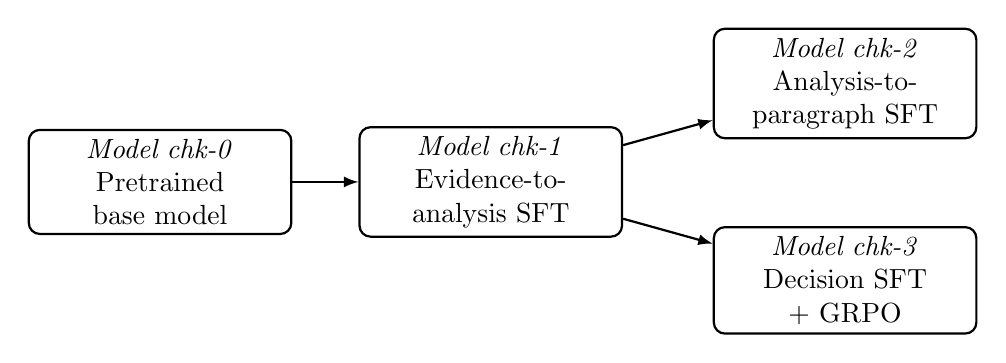
\begin{tikzpicture}[
        >=latex,
        model/.style={draw, rounded corners, align=center, text width=3.1cm,
            minimum height=1.25cm},
        every path/.style={->, thick}
    ]
        \node[model] (chk0) at (0,0)
            {\textit{Model chk-0}\\Pretrained base model};
        \node[model] (chk1) at (4.2,0)
            {\textit{Model chk-1}\\Evidence-to-analysis SFT};
        \node[model] (chk2) at (8.7,1.25)
            {\textit{Model chk-2}\\Analysis-to-paragraph SFT};
        \node[model] (chk3) at (8.7,-1.25)
            {\textit{Model chk-3}\\Decision SFT + GRPO};
        \draw (chk0) -- (chk1);
        \draw (chk1) -- (chk2);
        \draw (chk1) -- (chk3);
    \end{tikzpicture}
    \caption{Final paper-level training lineage.}
    \label{fig:ch2:training_stage1}
\end{figure}

Figure~\ref{fig:ch2:training_process} expands the lineage into the data and
optimization flows for analytical SFT and the two downstream tasks. The
retained diagrams use the original experimental identifiers: the
\textit{Model chk-3} and \textit{Model chk-4} labels printed in the graphics
correspond, respectively, to the paper-level \textit{Model chk-2} and
\textit{Model chk-3}. In addition, the ``Minutes'' box in the decision panel is
an earlier project-side shorthand; the finalized decision model receives the
target-neutral, pre-meeting analysis specified later in this section.

\begin{figure}[H]
    \centering
    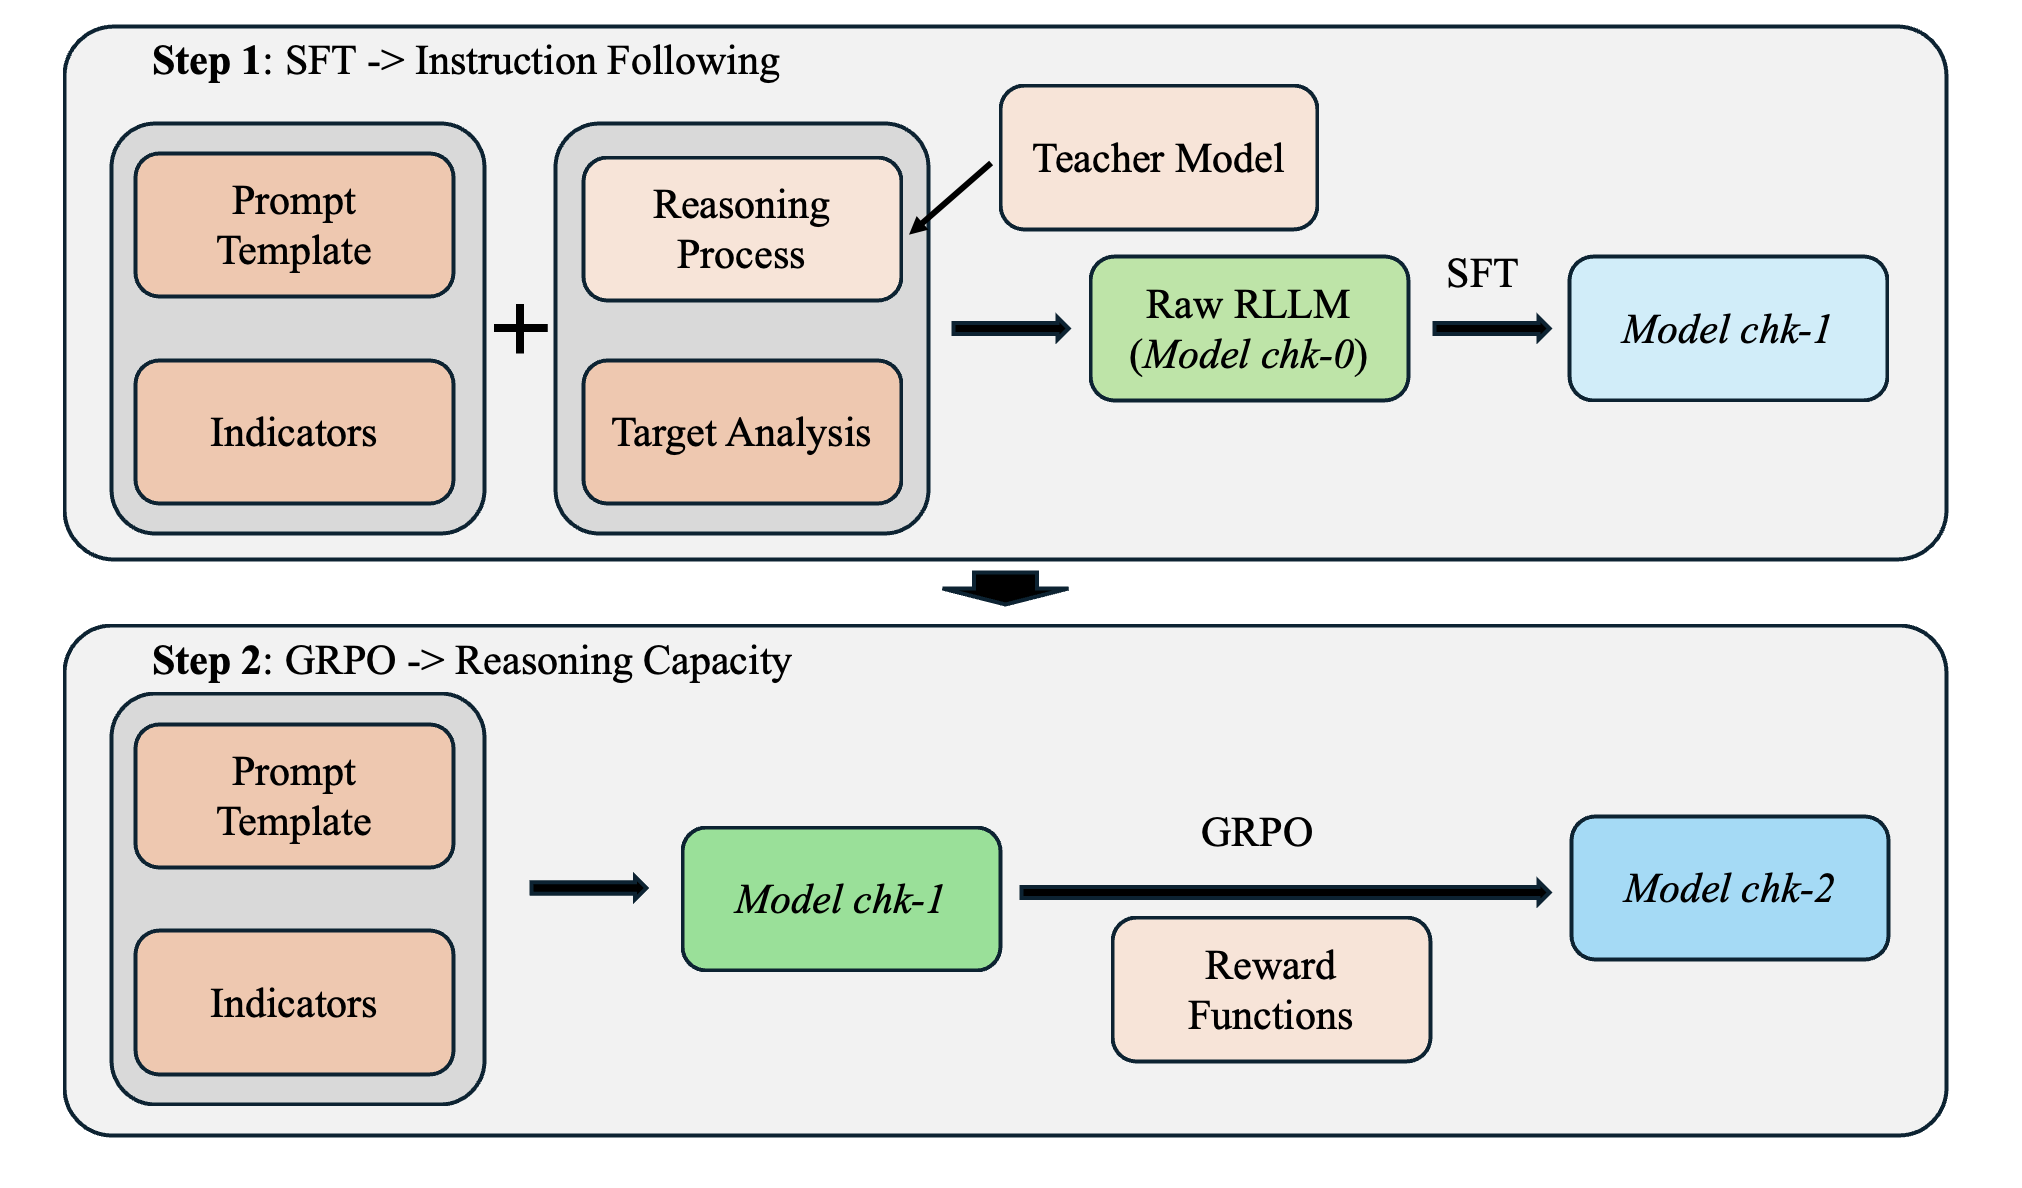
\includegraphics[width=\textwidth]{train/stage1.png}
    \par\medskip
    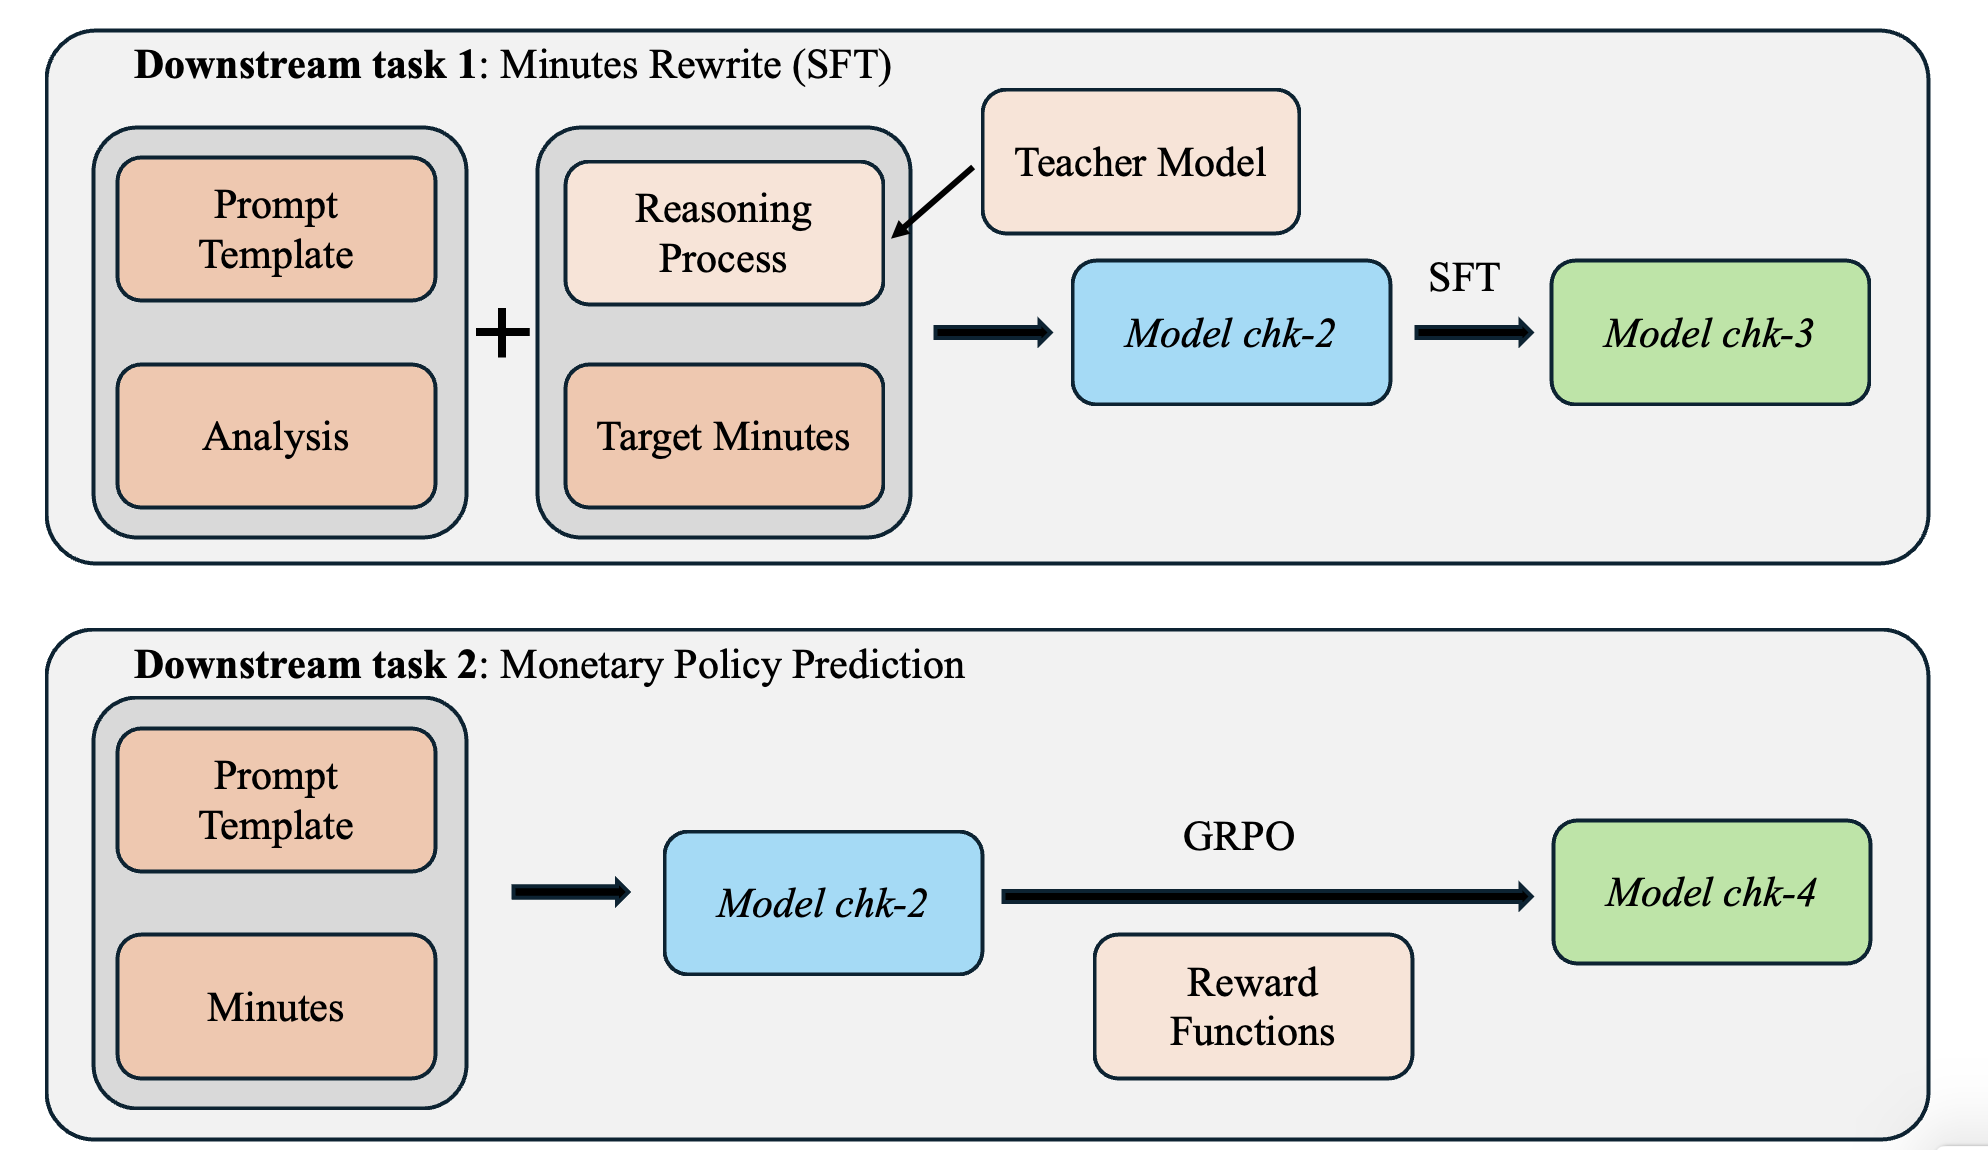
\includegraphics[width=\textwidth]{train/stage2.png}
    \caption{Overview of Two-step Training Process}
    \label{fig:ch2:training_process}
\end{figure}


%SFT
\paragraph*{Supervised fine-tuning.}
SFT adapts the model to the macro-financial tasks by learning from paired
prompts and reference completions. Each training example contains a system
instruction, a user prompt, and a target assistant response. The model is
optimized under teacher forcing, while parameter-efficient adapters reduce
the number of trainable parameters. Figure~\ref{fig:ch2:ft_detail} summarizes
this workflow.


\begin{figure}
    \begin{center}
        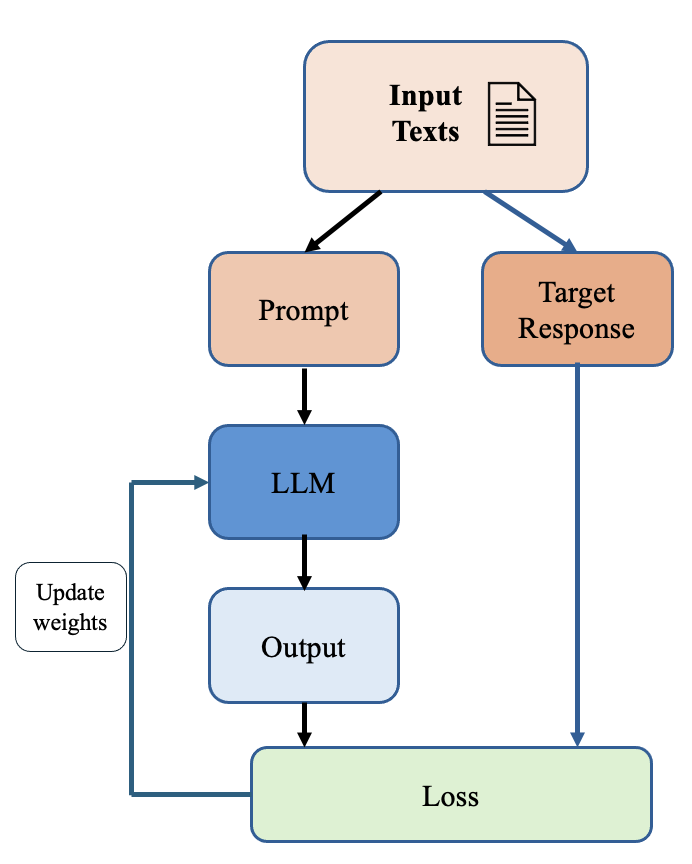
\includegraphics[width=0.3\textwidth]{Chapter2/Chapter2Figs/ft_detail.png}
      \end{center}
      \caption{Supervised fine-tuning workflow.}
      \label{fig:ch2:ft_detail}
\end{figure}



During SFT, let $x=(x_1,\ldots,x_M)$ denote the serialized prompt and
$y=(y_1,\ldots,y_N)$ the target assistant completion. At each target
position, the model predicts a distribution over the vocabulary conditional
on the prompt and preceding target tokens. The mean token-level negative
log-likelihood is
\begin{equation}
    \mathcal{L}_{\mathrm{SFT}}(\theta)
    =
    -\frac{1}{W}
    \sum_{t=1}^{N}
    w_t
    \log \pi_\theta\!\left(y_t\mid x,y_{<t}\right),
    \qquad
    W=\sum_{t=1}^{N}w_t,
\end{equation}
where $w_t\in\{0,1\}$ masks padding and any positions excluded from the
supervised objective. If every completion token is trained, $w_t=1$ and
$W=N$. Thus, SFT minimizes the negative log-probability assigned to the
reference completion; it does not compare a separately decoded response with
the target text.


%RL
\paragraph*{Reinforcement learning.}
Unlike SFT, policy optimization does not require a token-level reference
completion. In the decision task, however, the reference action remains
available to the deterministic reward function: the policy sees the prompt,
whereas the target direction and magnitude are used only to score sampled
completions.

Proximal Policy Optimization (PPO; \cite{schulman2017proximal}) stabilizes
policy-gradient updates by clipping the importance-sampling ratio. Let
$s_t=(q,o_{<t})$ be the token-generation state and define
\begin{equation*}
    \rho_t(\theta)
    =
    \frac{\pi_\theta(o_t\mid s_t)}
         {\pi_{\theta_{\mathrm{old}}}(o_t\mid s_t)}.
\end{equation*}
The clipped policy objective is
\begin{equation}
    \mathcal{J}_{\mathrm{PPO}}(\theta)
    =
    \mathbb{E}_t\!\left[
        \min\!\left(
            \rho_t(\theta)\widehat{A}_t,
            \operatorname{clip}
            \bigl(\rho_t(\theta),1-\epsilon,1+\epsilon\bigr)
            \widehat{A}_t
        \right)
    \right].
\end{equation}
Here, $\widehat{A}_t$ is an advantage estimate rather than the reward itself;
clipping constrains the policy ratio rather than rescaling the reward.




GRPO (\cite{shao2024deepseekmath}) removes the learned value function. For
each prompt $q$, the behavior policy samples a group
$\{o_i\}_{i=1}^{G}$, and the task reward assigns one terminal score
$R_i=R(q,y,o_i)$ to each completion. The group-relative advantage is
\begin{equation}
    \widehat{A}_i
    =
    \begin{cases}
    \displaystyle\frac{R_i-\overline{R}}{s_R+\eta}, & s_R>0,\\[7pt]
    0, & s_R=0,
    \end{cases}
    \qquad
    \overline{R}=\frac{1}{G}\sum_{j=1}^{G}R_j,
\end{equation}
where $s_R$ is the within-group reward standard deviation and $\eta>0$ is a
numerical stabilizer. The same completion-level advantage is applied to every
generated token in $o_i$. A group whose completions all receive the same
reward therefore supplies no group-relative learning signal.




For token $t$ of completion $i$, define
\begin{equation*}
    \rho_{i,t}(\theta)
    =
    \frac{\pi_\theta(o_{i,t}\mid q,o_{i,<t})}
         {\pi_{\theta_{\mathrm{old}}}(o_{i,t}\mid q,o_{i,<t})}.
\end{equation*}
A sampled per-token estimator for the KL regularizer is
\begin{equation*}
    \widehat{D}_{\mathrm{KL},i,t}
    =
    \frac{\pi_{\mathrm{ref}}(o_{i,t}\mid q,o_{i,<t})}
         {\pi_\theta(o_{i,t}\mid q,o_{i,<t})}
    -\log
    \frac{\pi_{\mathrm{ref}}(o_{i,t}\mid q,o_{i,<t})}
         {\pi_\theta(o_{i,t}\mid q,o_{i,<t})}
    -1.
\end{equation*}
Using
\begin{equation*}
    \ell_{i,t}(\theta)
    =
    \min\!\left(
        \rho_{i,t}(\theta)\widehat{A}_i,
        \operatorname{clip}
        \bigl(\rho_{i,t}(\theta),1-\epsilon,1+\epsilon\bigr)
        \widehat{A}_i
    \right)
    -\beta\widehat{D}_{\mathrm{KL},i,t},
\end{equation*}
the original sequence-normalized GRPO objective can be written as
\begin{equation}
    \mathcal{J}_{\mathrm{GRPO}}(\theta)
    =
    \mathbb{E}\!\left[
        \frac{1}{G}\sum_{i=1}^{G}
        \frac{1}{|o_i|}\sum_{t=1}^{|o_i|}
        \ell_{i,t}(\theta)
    \right].
\end{equation}

The completed decision run instead sets \texttt{loss\_type=dapo}. In this
trainer setting, DAPO denotes token-level loss aggregation: the losses are
normalized by the number of active completion tokens in the accumulated
training batch rather than separately by each completion length. If
$\mathcal{C}$ is the set of unmasked completions in that batch, the realized
aggregation is
\begin{equation}
    \mathcal{J}_{\mathrm{DAPO}}(\theta)
    =
    \mathbb{E}\!\left[
        \frac{\displaystyle
            \sum_{i\in\mathcal{C}}\sum_{t=1}^{|o_i|}\ell_{i,t}(\theta)}
             {\displaystyle
            \sum_{i\in\mathcal{C}}|o_i|}
    \right].
\end{equation}
This setting is related to the token-level aggregation proposed in DAPO
(\cite{yu2025dapo}), but it does not imply that the run adopted the complete
DAPO recipe. The realized configuration retained symmetric clipping and a KL
penalty; its numerical settings are reported with the decision-training
configuration below.





\subsection*{Analytical and Downstream Training}

\subsubsection*{Supervised Fine-tuning for the Analytical Model}

\paragraph*{Model chk-1.}
The first SFT stage adapts \textit{Model chk-0} to point-in-time
macro-financial analysis. Each supervised example is a pair
$(q_i,o_i^{\mathrm{SFT}})$, where $q_i$ is the model-visible prompt and
$o_i^{\mathrm{SFT}}=(c_i,a_i)$ is the reference assistant completion. Here,
$c_i$ denotes the reasoning prefix and $a_i$ the concise final analysis. This
distinction separates the model input from the supervision target. Training
for a small number of epochs limits, but does not eliminate, the risk that the
model memorizes task-specific wording.



Moreover, each LLM requires a model-specific message format, because tokenizers encode role boundaries differently. Explicit role labels are used specifically to distinguish the sections: the ``\texttt{System Prompt}'', ``\texttt{User Prompt}'', and ``\texttt{Assistant Response}''. Table. \ref{tab:ch2:input_template_for_llama3} presents the labels used by LLAMA3, where ``\prompttag{start\_header\_id}'' and ``\prompttag{end\_header\_id}'' wrap around the role labels indicating the message type. The label ``\prompttag{begin\_of\_text}'' signals the start of the conversation, while ``\prompttag{end\_id}'' denotes its end.



\begin{table}[h]
    \centering
    \footnotesize
    \begin{tabular}{p{0.98\textwidth}}
    \toprule
    \textbf{Special Labels for LLaMA 3:} \\
    \midrule
    \prompttag{begin\_of\_text} \\
    \prompttag{start\_header\_id} \textcolor{red}{system}\prompttag{end\_header\_id} \\
    \texttt{... System Prompts ...} \\
    \prompttag{start\_header\_id} \textcolor{red}{user}\prompttag{end\_header\_id} \\
    \texttt{... User Prompts ...} \\
    \prompttag{start\_header\_id} \textcolor{red}{assistant}\prompttag{end\_header\_id} \\
    \texttt{... Assistant Response ...} \\
    \prompttag{end\_id} \\
    \bottomrule
    \end{tabular}
    \caption{Input Template for LLAMA3}
    \label{tab:ch2:input_template_for_llama3}
\end{table}



\paragraph*{Reasoning boundary and final answer.}
The supervised completions follow the model's native reasoning-boundary
convention. A nonempty reasoning prefix $c_i$ is followed by exactly one
literal \texttt{</think>} marker and a nonempty final
answer $a_i$. Writing the boundary token as $b_{\mathrm{think}}$, the
serialized completion is
\begin{equation*}
    o_i=c_i\;\Vert\;b_{\mathrm{think}}\;\Vert\;a_i,
\end{equation*}
where $\Vert$ denotes string concatenation,$b_{\mathrm{think}} = \texttt{</think>} $. The semantic form of $a_i$ is task-specific: prose for \textit{Models chk-1} and \textit{chk-2}, and a decision object for \textit{Model chk-3}. 






\subsubsection*{Further Training for Downstream Tasks}

We adapt \textit{Model chk-1} separately for two downstream tasks. SFT on
analysis-to-FOMC-Minutes-style paragraph pairs produces \textit{Model chk-2}.
A separate branch uses decision SFT followed by GRPO to produce
\textit{Model chk-3}, which
predicts the direction and magnitude of a federal funds rate action.


\paragraph*{FOMC-Minutes-Style Paragraph Rewriting (\textit{Model chk-2})}

The Minutes-rewriting branch begins from the exact-merged \textit{Model chk-1}  and applies task-specific supervised fine-tuning to learn an analysis-to-paragraph transformation. 

First of all, because official FOMC Minutes often contain substantial details absent from the corresponding economic-analysis passages used as training inputs, treating the Minutes directly as targets would create misaligned supervision. We therefore used a teacher model to reconstruct a factually complete, de-styled analysis from each Official Minutes paragraph, ensuring that the student learns stylistic rewriting rather than supplying missing facts.

Then, for each training instance, the student model receives a fixed system instruction and a user message containing the analysis to be rewritten. Under teacher forcing, the target completion consists of a fidelity-planning reasoning section, one literal \texttt{</think>} boundary, and a single rewrote formal FOMC Minutes paragraph. The optimization objective therefore emphasizes the preservation of claims, quantities, dates, directions, comparisons, and uncertainty while adapting the output to the institutional style and structure of the FOMC Minutes. 




\paragraph*{Monetary Policy Decision Making (\textit{Model chk-3})}

The monetary-policy decision branch begins independently from the exact-merged \textit{Model chk-1} and proceeds through decision-specific SFT followed by GRPO. During SFT, the model receives a fixed system instruction and a user message containing a target-neutral pre-meeting analysis. The supervised completion consists of a qualitative dual-mandate rationale, one literal \texttt{</think>} boundary, and a terminal object specifying the policy direction and magnitude. GRPO then initializes from decision SFT checkpoint, retains the same model-facing prompt, action space, and response contract, and optimizes the parser-contingent decision proxy reward. 



\subsection*{Technique for Parameter-Efficient Fine-Tuning (PEFT)}

Full-parameter fine-tuning updates every model parameter and must retain the
associated gradients and optimizer states. Parameter-efficient fine-tuning
instead freezes the pretrained weights and optimizes a much smaller set of
task-specific parameters.

We use Low-Rank Adaptation (LoRA; \cite{hu2021lora}). For a pretrained linear
transformation with weight
$W\in\mathbb{R}^{d_{\mathrm{out}}\times d_{\mathrm{in}}}$, LoRA represents
the trainable update as
\begin{equation}
    W'=W+\Delta W,
    \qquad
    \Delta W=\frac{\alpha}{r}BA,
\end{equation}
where $A\in\mathbb{R}^{r\times d_{\mathrm{in}}}$,
$B\in\mathbb{R}^{d_{\mathrm{out}}\times r}$, and
$r\ll\min(d_{\mathrm{in}},d_{\mathrm{out}})$. The pretrained matrix $W$
remains frozen; only the low-rank factors are optimized.

Quantized Low-Rank Adaptation (QLoRA; \cite{dettmers2024qlora}) combines LoRA
with a quantized frozen base model; its 4-bit NormalFloat (NF4) representation
is distinct from generic FP4. The final training record for \textit{chk-2}
checkpoint 50 verifies NF4 QLoRA training with double quantization and
BF16 compute and storage, using a rank-32, $\alpha=64$ LoRA adapter with
dropout 0.05 on \texttt{q\_proj},
\texttt{k\_proj}, \texttt{v\_proj}, \texttt{o\_proj},
\texttt{gate\_proj}, \texttt{up\_proj}, and \texttt{down\_proj}. The main
text-similarity evaluation loads this adapter over the exact-merged
\textit{chk-1} checkpoint 200 parent in BF16 without inference quantization;
the \textit{chk-2} adapter itself remains active rather than being merged.
An adapter may remain
separate from its parent model or be merged for deployment; merging does not
by itself reduce the size of the resulting base-sized model.




\subsection{Training Hyperparameters}\label{ch2:sec:parameter}

Table~\ref{tab:ch2:training_hyperparameters_archive} reports checkpoint
identities and configuration values. 

\begin{table}[H]
    \centering
    \footnotesize
    \setlength{\tabcolsep}{3pt}
    \renewcommand{\arraystretch}{1.16}
    \begin{tabularx}{\textwidth}{@{}
        >{\centering\arraybackslash}p{0.08\textwidth}
        >{\centering\arraybackslash}p{0.08\textwidth}
        >{\raggedright\arraybackslash}p{0.18\textwidth}
        >{\raggedright\arraybackslash}p{0.18\textwidth}
        >{\raggedright\arraybackslash}X
    @{}}
        \toprule
        \textbf{Model} & \textbf{Stage} & \textbf{Initialization} &
        \textbf{Selected Point} &
        \textbf{Configuration} \\
        \midrule
        \textit{chk-1} & SFT & \textit{chk-0} & Checkpoint 200 selected and
        exact-merged & Final evaluation records fix the artifact identity;
        full training settings are not bound in the current record set. \\
        \textit{chk-2} & SFT & Exact-merged \textit{chk-1} checkpoint 200 &
        Checkpoint 50 selected by the validation-probe rule; active adapter &
        NF4 QLoRA $r=32$, $\alpha=64$, dropout 0.05; learning rate
        $10^{-6}$; three epochs (60 optimizer steps); completion-only loss.
        Selection evidence is reported in Appendix~\ref{app:checkpoint_selection}. \\
        \textit{chk-3} & SFT & Exact-merged \textit{chk-1} checkpoint 200 &
        Checkpoint 38 initializes GRPO & 211 unique meetings, 312 physical
        training rows. \\
        \textit{chk-3} & GRPO & Decision SFT checkpoint 38 & Run completed at
        step 468; checkpoint 450 used for evaluation &
        \texttt{loss\_type=dapo}; within-group scaling; four generations per
        prompt; generation batch 8; temperature 0.7; top-$p$ 0.9;
        $\beta=0.04$; $\epsilon=0.2$; prompt/completion limits 2,560/1,536;
        truncated completions masked; sole proxy reward
        \texttt{decision\_dense\_v3} with external weight 1.0. \\
        \bottomrule
    \end{tabularx}
    \caption{Paper-level model lineage and verified subset of the training configuration.}
    \label{tab:ch2:training_hyperparameters_archive}
\end{table}





\section{Model Evaluation Methods}\label{ch2:sec:application}


In this section, we evaluate the fine-tuned LLM's outputs with a focus on reliability. Given that LLMs are probabilistic generators, which selects the next token based on the highest probability, a critical issue encountered is the phenomenon known as hallucination. Hallucination refers to instances where the content generated by the model is unsupported by or conflicts with factual information. \cite{huang2025survey} have identified two primary forms of hallucination in LLMs: factuality hallucination and faithfulness hallucination. Factuality hallucination occurs when generated content contradicts real-world facts, whereas faithfulness hallucination arises when the generated content does not align consistently with the provided input. Consequently, tests designed to detect hallucinations are essential for evaluating the reliability of LLMs.




LLM evaluation can be broadly classified into reference-based and reference-free evaluation. First, reference-based evaluation compares the model’s outputs with target outputs generated under the same prompts. Scores are then used to quantitatively measure the differences between them. For example, the F1 score measures classification accuracy, BLEU \cite{papineni2002bleu} measures string-level overlap, and BERTScore \cite{zhang2019bertscore} measures semantic similarity based on token embeddings. Notably, reference outputs are required for reference-based evaluation. By contrast, reference-free evaluation does not require predefined target outputs. It is usually model-based or judgement-based, including regression-based validation between input prompts and outputs, LLM-as-Judge scoring, and human assessment.


Because fixed, source-grounded synthetic targets are available in this study,
we primarily use reference-based evaluation while treating target agreement as
distinct from fidelity to official FOMC Minutes. More specifically, we evaluate four
dimensions: (1) the \textbf{textual similarity} of generated outputs, (2)
\textbf{target-relative indicator sensitivity} under leave-one-out masking,
(3) exploratory \textbf{economic relevance} of synthetic text, and (4) the
\textbf{accuracy of policy-decision inference}.


The first dimension measures closeness to a reference text, while the second
measures local sensitivity to the conditioning inputs; neither alone
establishes factual grounding. The third and fourth dimensions provide
downstream checks on whether the generated text preserves economically
meaningful signals and supports inference of Federal Reserve decisions.



\subsection*{Evaluation Methods}

\subsubsection*{External Stochastic Evaluation of Minutes Rewriting}

The principal Minutes-rewriting evaluation uses an evaluation-only historical
release containing all 128 regular FOMC meetings from 1993 through 2008. One
Core8 topic prompt is assigned to each meeting, with exactly 16 prompts for
each of the eight topics. This release is external to the chapter-specific
fine-tuning and checkpoint-selection procedures, although it is not claimed to
be absent from the pretrained base model's corpus. The references are
deterministic, source-grounded Minutes-style targets rather than excerpts from
official FOMC Minutes.

The evaluation compares \textit{Model chk-0}, \textit{Model chk-1} checkpoint
200, and \textit{Model chk-2} (repository artifact \texttt{chk3}, checkpoint
318). The primary contrast is \textit{Model chk-2} minus its immediate
\textit{Model chk-1} parent; \textit{Model chk-0} is an auxiliary reference.
Each model generates ten stochastic continuations for every prompt, yielding
\(128\times10\times3=3{,}840\) completions. The decoding contract fixes
temperature at 0.6, top-$p$ at 0.95, top-$k$ at 50, and the maximum completion
length at 3,072 tokens. For each meeting and replicate, the same derived random
seed is used for all three models, so comparisons are paired by meeting,
prompt, replicate, and seed.

Four hard validity criteria are evaluated for every completion. Structural and
delivery validity requires normal termination, one properly delimited nonempty
rationale, and one plain-text paragraph. Numerical fidelity requires exact
preservation of the multiset of numerical quantities in the source analysis.
Date fidelity requires exact preservation of the source date set. The
degeneration criterion rejects a strictly periodic tail or excessive four-gram
repetition. A completion that fails any hard criterion is assigned zero for
both semantic-similarity measures.

For completions that satisfy all four hard criteria, semantic alignment is
measured using BERTScore F1 and MPNet cosine similarity between the generated
paragraph and its synthetic source-grounded target. The resulting semantic
statistics are therefore \emph{reliability-adjusted}: they combine successful
delivery with conditional semantic alignment and are not valid-only encoder
means. Semantic similarity does not by itself establish factual accuracy.

\subsubsection*{Textual Similarity}

Semantic alignment is evaluated against the synthetic teacher target used by
the Minutes-rewriting task.  Let \(Y_i\) denote the final paragraph generated
for observation \(i\), and let \(Y_i^{*}\) denote its corresponding synthetic
reference paragraph.  Two independently pretrained encoders are used.  First,
BERTScore F1 is computed with a frozen RoBERTa-large model by matching each
contextualized candidate token with the most similar reference token and vice
versa (\cite{zhang2019bertscore}).  Second, the generated and reference
paragraphs are embedded with the frozen
\texttt{sentence-transformers/all-mpnet-base-v2} encoder, and their cosine
similarity is calculated as

\begin{equation}
    Cos_i^{MPNet}
    =\frac{h(Y_i)^{\top}h(Y_i^{*})}
    {\lVert h(Y_i)\rVert_2\lVert h(Y_i^{*})\rVert_2},
\end{equation}

where \(h(\cdot)\) denotes the MPNet sentence embedding.  Both encoders are
fixed and independent of the models used to generate the training targets.
An observation that fails any preregistered structural, numerical, date, or
non-degeneration criterion receives a value of zero for both semantic metrics.

The completed experiment defines improvement relative to the
\textit{Model chk-1} checkpoint-200 baseline. For a metric
\(M\in\{BERTScore\text{-}F1,Cos^{MPNet}\}\), the observation-level contrast is

\begin{equation}
    \Delta M_i=M_i^{\mathrm{chk2}}-M_i^{\mathrm{chk1}}.
\end{equation}

Positive values favour \textit{Model chk-2}. Within each prompt, the ten
replicates are averaged first; the resulting prompt scores are then aggregated
with equal weight for each of the 128 meetings. Uncertainty is estimated with
2,000 hierarchical paired-bootstrap draws that resample meetings and, within
each sampled meeting, the stored replicates while preserving the same indices
across models and metrics. Two-sided Monte Carlo paired sign-flip tests use
100,000 deterministic sign assignments. The six primary
\textit{Model chk-2}-minus-\textit{Model chk-1} tests are corrected jointly by
the Holm procedure. These intervals capture meeting and decoding variation for
the frozen model artifacts, not uncertainty across independently trained model
runs.

% The material below records an earlier generic metric discussion and is
% excluded from the current experiment specification.
\iffalse

% Cosine Similarity
To start with, the textual similarity targets comparing the similarity between the target output and the generated output using mathematical distance, such as the Levenshtein Similarity Ratio (\cite{levenshtein1966binary}) and Cosine Similarity (\cite{tanguy2016natural}). The Levenshtein Similarity Ratio replies on the Levenshtein Distance to measure the minimum number of strings that need to be edited from the generated output to the required output. Furthermore, some other metrics driven from the idea of ``n-grams'', such as the Recall-Oriented Understudy for Gisting Evaluation score (ROGUE score, \cite{lin2004rouge}), provide an grammatical-level measurement than the word-level Levenshtein Similarity Ratio. These methods are useful at the age of ``Bag-Of-Word (BOG)''.

However, with the development of LLM, researchers can take advantage of the embeddings from the LLM rather than the one-hot key of ``BOG''. The embeddings can convert the ``word'' into tokens that encoded more semantic information than the one-hot key. Therefore, the Cosine Similarity provides a more accurate estimation of the semantic similarity between two texts. Here, we will use the \textit{sentence-level} \textbf{Cosine Similarity} as our first metric to evaluate the text similarity of outputs. Cosine Similarity ranges from 0 to 1, where a value of 1 indicates a perfect similarity between the two texts, while a value of 0 signifies that the texts are highly different from each other.

The metric helps in determining how well the generated text aligns with the expected content in terms of both meaning and context. For example, \cite{aynetdinov2024semscore}, \cite{kim2024comparison}, and \cite{yauney2023data} used the Cosine Similarity as a benchmark when evaluating the LLM's performance.

Cosine similarity is estimated by the cosine of the angle between two non-zero vectors. It is defined as the dot product of the two vectors divided by the product of their magnitudes. This mathematical operation helps in quantifying how closely the generated text aligns with the target text in terms of meaning and content. We utilize the ``tokenizer'' and the ``hidden layers'' from the LLAMA3 model to convert the response texts into vector representations, denoted as $Y$ for the target text and $\hat{Y}$ for the generated text.


%%% text embedding calculation

% tokens = [2, 1, 3]
% text_embedding = [[0.111, 0.232131, 0.41414, 0.2412424, 0.1424, 0.444, 0.99]
%                     [0.5151, 0.52215, 0.232132, 0.223232, 0.535151, 0.23231, 0.515151]
%                     [0.2155252, 0.2223, 0.54331, 0.321313, 0.14222, 0.421555, 0.535252]]
% mean pooling = [0.23131, 0.222, 0.23213, 0.325325, 0.532555, 0.535325, 0.23232, 0.424141]

% | 模型          | hidden_size | num_hidden_layers |
% | ----------- | ----------- | ----------------- |
% | BERT-base   | 768         | 12                |
% | Llama-7B    | 4096        | 32                |
% | GPT-3 small | 12288       | 96                |

% google-bert 768, [https://huggingface.co/google-bert/bert-base-uncased/blob/main/config.json]
% gemini3-27b 5376,, [https://huggingface.co/google/gemma-3-27b-it/blob/main/config.json]
% Deepseek-r1 7168,[https://huggingface.co/deepseek-ai/DeepSeek-R1/blob/main/config.json]
% llama3.1-70b  8192,




Compared with the ``one-hot encoding'' used in the ``Bag-of-Words'' model, the text embeddings employed in large language models (LLMs) offer two significant advantages. On the one hand, text embeddings employ a tokenizer to map the input text into a sequence of dense vectors, $\mathbf{h}_i \in \mathbb{R}^{m\times 1}$, where $i = 1, 2, ..., n$ corresponds to each token in the text, and $m$ denotes the hidden-layer dimension, rather than high-dimensional binary representations. On the other hand, the hidden layers within the LLM transform each token vector into a contextualized embedding by encoding both semantic meaning and positional information.

Noticeably, the hidden layer size ($m$) is different for different models. Generally, a larger hidden dimension allows the model to capture more fine-grained semantic information. For example, Google BERT (110M parameters) has a hidden size of 768 \cite{googlebert}, Gemini 3-27B has a hidden size of 5,376 \cite{googlegemini3}, and LLaMA 3.1-70B uses a hidden size of 8,192 \cite{metallama3}.


Furthermore, after the encoding stage, there is a pooling stage aimed at adjusting the dimension of text embedding matrix ($\mathbf{H} \in \mathbb{R}^{M\times N} = [\mathbf{h_1}, \mathbf{h_2}, ..., \mathbf{h_N}]$) to 1 ($\mathbf{H'} \in {\mathbb{R}^{M\times 1}}$). Then, this adjusted text embedding is a vector representation of the input text. Common pooling strategies include mean pooling, max pooling, and weighted-sum pooling. 

% During the pooling stage, token embeddings are aggregated—typically by averaging across all tokens—to produce a single fixed-length vector representing the entire input text. Common pooling strategies include mean pooling, max pooling, and weighted-sum pooling. 

% First, mean pooling computes the average embedding across all tokens:

% \begin{equation}\label{eq:ch2:mean_pooling}
%     h'_{j} = \frac{1}{N} \sum_{i=1}^{N} h_{ij}
% \end{equation}

% where $h_{ij}$ denotes the j-th dimension of the i-th token embedding.

% Second, max pooling selects the maximum value across all tokens for each embedding dimension:

% \begin{equation}\label{eq:ch2:max_pooling}
%     h'_{j} = Max(h_{1j}, h_{2j}, ..., h_{Nj})
% \end{equation}


% Finally, weighted-sum pooling computes a weighted average of token embeddings:

% \begin{equation}\label{eq:ch2:weight_sum_pooling}
%         h'_{j} = \frac{1}{N} \sum_{i=1}^{N} w_{i,j}h_{ij} 
% \end{equation}
% where $w_{ij}$ are non-negative weights satisfying $\sum_{i=1}^{N} w_{ij} = 1$ . In practice, attention weights from a pre-trained transformer are often used as $w_{ij}$.
 
To balance the effect of all the tokens, in this study, we adopt mean pooling. Max pooling tends to overemphasize a small number of highly activated tokens, while weighted-sum pooling can be dominated by tokens with disproportionately large attention weights. Mean pooling provides a more stable and balanced representation across the entire text. Appendix \ref{app:text_embedding} provides a detailed illustration and example for the text embedding generation process. 


Therefore, the cosine similarity score, denoted as $Cos_{Y, \hat{Y}}$, is then calculated as follows:


\begin{equation*}
    Cos_{Y, \hat{Y}} = \frac{Y \cdot \hat{Y}}{\|Y\|_2 \|\hat{Y}\|_2}
\end{equation*}


where $Y$ and $\hat{Y}$ are sentence embeddings for the reference and generated texts, and $\|\cdot\|_2$ denotes the Euclidean norm (e.g., $\|Y\|_2=\sqrt{y_1^2+y_2^2+\cdots+y_N^2}$).


% According to the distribution theory, 
Finally, drawing from distributional semantics theory (\cite{firth1957linguistics}, \cite{sahlgren2008distributional}), words with similar meanings tend to occur in similar contexts and thus have similar distributions in the vector space. Therefore, we hypothesize that texts with higher semantic likeness will exhibit a greater cosine similarity. 


% BERTScore 

On the other hand, in addition to Cosine Similarity, which serves as a \textit{sentence-level} metric, we also employ \textbf{BERTScore} (\cite{zhang2019bertscore}), a metric designed to capture \textit{token-level} semantic similarity using cosine similarity as its underlying distance measure.

More specifically, for each token $\hat{y}_j$ in the target (reference) output $\hat{Y}$, BERTScore identifies the maximum cosine similarity with respect to all candidate tokens $y_i$ in the generated response $Y$. These maximal token-level similarities are then aggregated to construct three complementary evaluation metrics: \textit{Recall} ($BertScore^{Recall}$), \textit{Precision} ($BertScore^{Precision}$), and the harmonic mean of the two, the \textit{F1 score} ($BertScore^{F1}$).


Let $Y=\{y_i\}$ denote the set of token embeddings in the generated response and $\hat{Y}=\{\hat{y}_j\}$ denote the set of token embeddings in the reference (target) text. BERTScore computes \textit{Precision} by matching each candidate token to its most similar reference token, and \textit{Recall} by matching each reference token to its most similar candidate token. Finally, the F1 Score (Eq.(\ref{eq:ch2:bert_f1})) is calculated as the harmonic mean of precision and recall, thereby providing a balanced measure of semantic alignment between the generated and reference texts:

\begin{equation}\label{eq:ch2:bert_precision}
    BERTScore^{Precision} = \frac{1}{\|Y\|}\sum_{y_i \in Y} \max_{\hat{y}_j \in \hat{Y}} y_i^{\text{T}}\hat{y}_j
\end{equation}

\begin{equation}\label{eq:ch2:bert_recall}
    BERTScore^{Recall} = \frac{1}{\|\hat{Y}\|}\sum_{\hat{y}_j \in \hat{Y}} \max_{y_i \in Y} \hat{y}_j^{\text{T}}y_i
\end{equation}

\begin{equation}\label{eq:ch2:bert_f1}
    BERTScore^{F1} = \frac{2\cdot BERTScore^{Precision}\cdot BERTScore^{Recall}}{BERTScore^{Precision}+BERTScore^{Recall}}
\end{equation}


For the completed Minutes-rewriting experiment, the directional hypotheses are
defined relative to the \textit{Model chk-1} baseline:

\begin{equation*}
    \begin{split}
        &Cos_{\mathrm{chk2}} - Cos_{\mathrm{chk1}} > 0 \\
        &BERTScore^{Recall}_{\mathrm{chk2}} - BERTScore^{Recall}_{\mathrm{chk1}} > 0 \\
        &BERTScore^{Precision}_{\mathrm{chk2}} - BERTScore^{Precision}_{\mathrm{chk1}} > 0\\
        &BERTScore^{F1}_{\mathrm{chk2}} - BERTScore^{F1}_{\mathrm{chk1}} > 0
    \end{split}
\end{equation*}


where subscripts \textit{chk2} and \textit{chk1} denote the task-specific model
and experimental baseline, respectively. These inequalities describe a
directional hypothesis about semantic alignment. Valid inference would require
paired row-level scores from a fixed test manifest that is independent of
checkpoint selection, together with an appropriate uncertainty estimator and
immutable checkpoint identities. Cosine similarity and BERTScore alone measure
resemblance to a reference; they do not establish factual, numerical,
directional, or reasoning fidelity.


%%%%% end of text similarity
\fi


\subsubsection*{Target-relative Indicator Sensitivity}
% Indicator-level leave-one-out sensitivity

Apart from textual similarity, we also require the generated output to reflect information supplied by the input indicators rather than relying solely on unsupported completion. The question in this subsection is therefore not only whether the generated section resembles the target text, but also whether removing a given indicator materially changes that resemblance.


To study this issue, our second metric evaluates how sensitive the generated
output's target alignment is to removing one complete indicator block.
Section~\ref{ch2:sec:lr:evaluation} distinguishes this intervention from
coalition-averaged Shapley attribution. For notation, the Shapley Value
($\mathcal{SV}$) is the expected marginal contribution of a feature ($p_i$)
to a model output $f(\cdot)$ (\cite{shapley1953value}):

\begin{equation*}
  \mathcal{SV}_i(f) = \sum_{\mathcal{S} \subseteq \mathcal{P}\setminus\{p_i\}} \frac{\left|\mathcal{S}\right|! (n - \left|\mathcal{S}\right| - 1)!}{n!} \left(f(\mathcal{S}\cup\{p_i\}) - f(\mathcal{S})\right)
\end{equation*}

where $\mathcal{P}=\{p_1, p_2, \cdots, p_n\}$ is the set of prompts, $\mathcal{S}$ is a coalition (subset) of prompts, and $f(\cdot)$ is a utility function. The term $f(\mathcal{S}\cup\{p_i\})-f(\mathcal{S})$ denotes the marginal contribution of feature $p_i$ to coalition $\mathcal{S}$.


In this research, however, we do not estimate the full Shapley Value across all possible coalitions. Instead, we use an \textbf{indicator-level leave-one-out masking test} (Leave-one-out test hereafter). We remove one complete indicator block at a time while holding the remaining prompt content fixed. This is a local sensitivity diagnostic under a specified masking intervention, not a Shapley Value and not by itself proof of grounding. Let $\mathcal{P}=\{p_1,\ldots,p_n\}$ denote the full indicator set, $o(\mathcal{P})$ the full-prompt output, $o(\mathcal{P}\setminus\{p_i\})$ the output after masking indicator $i$, and $y$ a target that is held fixed within the pair. With sentence-embedding cosine similarity, define

\begin{align}
 s_{\mathrm{full}} &= \operatorname{Cos}\!\left(o(\mathcal{P}),y\right), \nonumber\\
 s_{\mathrm{masked},i} &= \operatorname{Cos}\!\left(o(\mathcal{P}\setminus\{p_i\}),y\right), \nonumber\\
 \Delta_i &= s_{\mathrm{full}}-s_{\mathrm{masked},i}.
 \label{eq:ch2:loo_delta}
\end{align}

Equivalently, if cosine distance is $d=1-s$, then
$\Delta_i=d_{\mathrm{masked},i}-d_{\mathrm{full}}$. Thus,
$1-s_{\mathrm{masked},i}$ alone is the masked output's target-relative cosine
distance and is not the LOO contribution because it still contains the full
output's baseline distance. A positive $\Delta_i$ means that masking indicator $i$ reduces
target alignment; a negative value means that masking improves alignment.
Negative values are retained rather than truncated.

For the canonical Core8 target-relative analysis, $y$ is the fixed,
deterministic synthetic source-grounded target defined in the frozen external
panel. The two surviving legacy workbooks use different archived target
contracts and are reported separately: the internal-sensitivity workbook sets
$y=o(\mathcal{P})$, whereas the historical external-alignment workbook uses
the corresponding actual FOMC Minutes section. Under the internal contract,
$s_{\mathrm{full}}=1$ and
$\Delta_i=1-\operatorname{Cos}(o(\mathcal{P}\setminus\{p_i\}),o(\mathcal{P}))$,
which measures change relative to the model's own unmasked output. These
legacy estimands are not interchangeable with the canonical synthetic-target
estimand. In a new canonical run, full and masked generations will be paired
by meeting, indicator, and generation replicate, and both component scores
and the signed delta will be retained. Rows will first be averaged within each
meeting--replicate cell,
replicates will then receive equal weight in the meeting mean, confidence
intervals will resample meetings, and one global Holm family will cover all
reported indicator--section--context cells in the run. The intervention
manifest will bind every generated row to its prompt hash, verify that the
deleted complete block begins with a roster-declared marker for the named
indicator, reject overlapping deletion spans and duplicate masked prompts
across indicators, and fingerprint both the generation checkpoint and
embedding model.


%%%% end of leave-one-out definition

\subsubsection*{Exploratory Association Test using Synthetic Texts}


Section~\ref{ch2:sec:lr:communication} distinguishes event studies of observed
FOMC releases from predictive and reduced-form text-as-data designs. Motivated
by that literature, this exploratory association test asks whether sentiment
extracted from synthetic Minutes preserves the direction of a historical
text--market relationship. Because the synthetic text was not released at the
historical event time, the exercise cannot identify a market response caused
by the generated text. Nor can statistical significance in this regression,
by itself, establish realistic or factually grounded Minutes generation. The
test is therefore a cross-artifact coefficient diagnostic, not a test of the
model's institutional simulation capacity.



We adapt the reduced-form specification in \citet{tadle2022fomc}, which relates
sentiment in observed FOMC communications to movements in interest and
exchange rates. Equation~\ref{eq:ch2:sentiment_reg} is used here only as a
descriptive coefficient-pattern diagnostic across text artifacts. Because the
synthetic Minutes were not observed by market participants, their coefficients
are associations conditional on the included controls, not market effects. A
verified cross-artifact comparison would additionally require a common frozen
sample, checkpoint binding, resampling unit, and direct model-difference test;
the surviving legacy record does not retain all of those elements.



\begin{equation}\label{eq:ch2:sentiment_reg}
    p^f_t = \lambda p^f_{t-1} + \alpha + \beta_{Z_t^M} Z_t^M+ \beta_{Z_{t-1}^M} Z_{t-1}^M + \beta_{Z_t^S} {Z_t}^S + \beta_{VIX_t}VIX_t + \beta_{Y_t}Y_t + \phi_t 
\end{equation}



where $p^f_t$ is the price for the Federal Fund Rate Future contract $f$ at time $t$. $VIX_t$ is the log change of the Volatility Index (VIX), $Z_t^M$ and $Z_t^S$ are the sentiment scores extracted from the Minutes and Statements, $Y_t$ is the monthly time effect, and $\phi_t$ is the error term.

Following the empirical test, a bootstrap procedure estimates the distribution of the $\beta$ coefficients. A fully identified comparison would additionally require the exact source series, resampling unit, model manifest, and uncertainty for the difference between model-derived coefficients. The surviving legacy outputs do not retain all of these elements, so the archived plots are reported later only as exploratory and unverified.



%%%% end of statistical significant



\subsubsection*{Evaluation of the Policy-Decision Branch}

The decision exercise is a meeting-level historical classification task, not
a causal test of institutional simulation. The frozen release contains 237
unique meetings: 211 training meetings, 13 validation meetings, and 13 test
meetings. The evaluation compares the common parent, \textit{Model chk-1}
checkpoint 200, with the pre-GRPO SFT state of \textit{Model chk-3} at
checkpoint 38 and its evaluated post-GRPO state at checkpoint 450. All three
models are scored on identical meeting identifiers. The 13-meeting
training-held-out test split is the primary quality check; the complete
237-meeting comparison is a secondary within-release diagnostic because
211/237 meetings, or 89.03\%, belong to the training split.

For each meeting, the model receives exactly the fixed system instruction and
the one-field, target-neutral pre-meeting analysis payload documented in
Table~\ref{tab:chk3-decision-sft-example}. The model does not receive a
separate meeting-date or current-rate field, sample identifier, split label,
target action, scoring rule, reward coefficients, a few-shot answer, or another
model's output. Publicly observable pre-meeting policy state may still appear
inside the analysis. The local direction-and-magnitude label remains hidden until
deterministic post-generation scoring. Target-neutrality excludes direct
target-meeting fields, known realized outcomes, and post-meeting observations;
it does not prove that a sufficiently knowledgeable model could not infer a
meeting or period indirectly from the supplied economic context.

The admissible action set contains \texttt{hold:0} and cuts or hikes of 25,
50, 75, or 100 basis points. A model completion must contain a nonempty native
reasoning prefix, one \texttt{</think>} boundary, and a terminal JSON object
with exactly the keys \texttt{direction} and \texttt{magnitude\_bp}. Direction
must be \texttt{cut}, \texttt{hold}, or \texttt{hike}; a hold requires zero
magnitude. Invalid or undelivered responses remain errors in every reported
denominator.

Decision quality is summarized by direction accuracy, fixed-three-class
balanced accuracy, fixed-three-class macro F1, and exact direction-and-
magnitude accuracy. Output reliability is reported separately as the strict
JSON and delivery-valid rate. The training-held-out test table reports point
estimates because its 13 meetings are too few for stable split-specific
inference and the split has already been opened. For the secondary all-237
diagnostic, model differences use 10,000 target-direction-stratified,
meeting-paired bootstrap draws. These intervals describe within-release model
differences; they are not estimates of performance on future meetings.








\section{Empirical Results}\label{ch2:sec:result}

This section reports the completed training evidence and the external
stochastic evaluation of FOMC-Minutes rewriting. It then evaluates the
independent policy-decision branch under its frozen prompt and common meeting
population. The Minutes and decision results answer separate questions and are
not interpreted as a serial end-to-end pipeline.


\subsection*{Model Training Results}

\subsubsection*{Step 1: Supervised Fine-Tuning (SFT) Results (\textit{Model chk-1})}

The first SFT stage fine-tunes DeepSeek-R1-Distill-Llama-8B on 1,354 training
observations.  As discussed in Section~\ref{ch2:sec:the-dataset}, this sample
satisfies the structural validation criteria but is used subject to the
qualification raised by the strict source-grounding audit.  The model is
estimated using completion-only QLoRA for three epochs, with a peak learning
rate of \(1.0\times10^{-6}\)\footnote{The staged learning-rate stability
diagnostics are reported in Appendix~\ref{app:checkpoint_selection},
Table~\ref{tab:app:chk1_lr_stability}.}, a maximum sequence length of 7,168 tokens, a
per-device batch size of 1, and gradient accumulation over 8 steps.  Training
terminates after 255 optimization steps, with a mean training loss of
1.777860.  Validation is conducted periodically on a fixed sample of 199
observations.

Checkpoint 200 is selected instead of the final checkpoint because it attains
the lowest validation loss, 1.686099, with a token accuracy of 0.602685.  It
also satisfies all generation-validity criteria in the eight-observation
diagnostic sample: every completion terminates normally, conforms to the
response format, remains below the token limit, and avoids periodic or
catastrophic repetition.  Its mean token four-gram repetition rate is
0.134664, compared with 0.1410 at checkpoint 255.  The final checkpoint has a
validation loss of 1.686131, only 0.000032 above the minimum.  The training
trajectory is therefore more consistent with a validation plateau than with a
substantive late-stage deterioration, while the repetition diagnostic provides
a secondary reason to prefer checkpoint 200.

These results establish that the SFT objective is optimized stably and that the
selected model satisfies the basic generation criteria on the diagnostic
sample.  They should not, however, be interpreted as evidence of factual
accuracy on the held-out test set.


\subsubsection*{Minutes-Rewriting SFT Results (\textit{Model chk-2})}

The Minutes-rewriting experiment estimates the task-specific paper-level
\textit{Model chk-1} $\rightarrow$ \textit{Model chk-2} transition. It is
initialized from \textit{Model chk-1} checkpoint 200 and trained on the
analysis-to-Minutes dataset
described in Section~\ref{ch2:sec:the-dataset}.  The response target comprises
a synthetic teacher-generated fidelity rationale followed by a paragraph in
the style of the FOMC Minutes, rather than an excerpt from the official
Minutes.  Estimation uses completion-only
QLoRA for three epochs, with a learning rate of \(1.0\times10^{-6}\), a
maximum sequence length of 4,096 tokens, a per-device batch size of 1, and
gradient accumulation over 8 steps.  The training procedure terminates after
318 optimization steps.

Validation loss alone favoured checkpoint 250. Exact-merged replay on the
fixed twelve-observation diagnostic, however, found one capped periodic
completion as well as numerical and date failures at that checkpoint.
Checkpoint 318 is the only exact-merged finalist that satisfies all four hard
validity criteria for all 12 observations, while its validation loss is only
0.000076 above the observed minimum. It is therefore retained for external
evaluation. The complete candidate table and the auxiliary semantic diagnostic
are reported in Appendix~\ref{app:checkpoint_selection}. Because the same
small deterministic sample participates in checkpoint selection, it provides
no population-level evidence about rewriting performance.



\subsubsection*{Policy-Decision Training States (\textit{Model chk-3})}

The decision branch starts independently from \textit{Model chk-1} checkpoint
200 and never consumes outputs from \textit{Model chk-2}. Decision SFT uses the
fixed 312-row exposure schedule for 39 optimizer steps; exact-merged checkpoint
38 is retained as the pre-GRPO state. GRPO then starts from checkpoint 38, uses
the same 312-row decision population for three epochs and four generations per
prompt, and terminates at global step 468 under the deterministic
\texttt{decision\_dense\_v3} proxy objective.

Checkpoint 450 is evaluated because it is the best-observed exploratory
candidate in the completed probe, not because it passed the preregistered
selection gates. Its blind delivery-valid rate is 0.30, below the 0.75 gate;
the authoritative record therefore reports
\texttt{selected\_checkpoint\_step=null} and
\texttt{status=provisional\_no\_candidate\_passed\_all\_gates}. The subsequent
test verdict is \texttt{quality\_not\_demonstrated}. Accordingly, checkpoint
450 is an evaluated post-GRPO state, not a selected or promoted model.






\subsubsection*{Training Results Summary}

The supervised-training evidence establishes \textit{Model chk-1} as the
common parent of the Minutes and decision branches. \textit{Model chk-2}
(repository artifact \texttt{chk3}, checkpoint 318) is assessed on the external
Minutes-rewriting release. The two successive states of \textit{Model chk-3}
(repository artifact \texttt{chk4}) are assessed separately on the decision
task: checkpoint 38 before GRPO and checkpoint 450 after GRPO. Training losses
and proxy rewards document optimization of their own objectives; they are not
substitutes for the task-level evaluations below.



%%% end of decision making



\subsection*{Model Evaluation Results}

The principal completed evaluation compares \textit{Model chk-2} with its
\textit{Model chk-1} parent on the external 1993--2008 release. The policy-
decision branch is evaluated separately under its own frozen sample and output
contract.

\subsubsection*{External Stochastic Minutes-Rewriting Performance}

Table~\ref{tab:ch2:minutes_external_n128_k10} reports meeting-equal-weight
results for 128 meetings and ten stochastic replicates per meeting and model.
The semantic columns incorporate the preregistered zero penalty whenever a
completion fails at least one hard validity gate.

\begin{table}[htbp]
    \centering
    \scriptsize
    \setlength{\tabcolsep}{2.7pt}
    \renewcommand{\arraystretch}{1.15}
    \begin{tabularx}{\textwidth}{@{}>{\raggedright\arraybackslash}Xrrrrrr@{}}
        \toprule
        \textbf{Metric} & \makecell{\textit{Model}\\\textit{chk-0}} &
        \makecell{\textit{Model chk-1}\\cp200} &
        \makecell{\textit{Model chk-2}\\cp318} &
        \makecell{chk-2\\minus chk-1} & \textbf{Paired 95\% CI} &
        \makecell{Holm\\$p$} \\
        \midrule
        Structure/delivery & 0.992188 & 0.993750 & 0.997656 & +0.003906 & $[-0.002344,\ 0.010938]$ & 0.672743 \\
        Numeric fidelity & 0.394531 & 0.404688 & 0.460938 & +0.056250 & $[0.018750,\ 0.094531]$ & 0.000360 \\
        Date fidelity & 0.981250 & 0.981250 & 0.980469 & $-0.000781$ & $[-0.014844,\ 0.011738]$ & 1.000000 \\
        Degeneration-free & 0.999219 & 0.998438 & 0.997656 & $-0.000781$ & $[-0.005469,\ 0.003906]$ & 1.000000 \\
        MPNet, reliability-adjusted & 0.337012 & 0.345137 & 0.406584 & +0.061446 & $[0.029393,\ 0.095796]$ & 0.000060 \\
        BERTScore-F1, reliability-adjusted & 0.358354 & 0.368022 & 0.425153 & +0.057130 & $[0.023620,\ 0.093240]$ & 0.000200 \\
        \bottomrule
    \end{tabularx}
    \caption{External Stochastic Evaluation of Minutes Rewriting (128 Meetings, 10 Replicates per Model). The primary contrast is \textit{Model chk-2} minus \textit{Model chk-1}; \textit{Model chk-0} is auxiliary. Semantic scores are reliability-adjusted and are set to zero after any hard-gate failure. References are synthetic source-grounded targets, not official FOMC Minutes. The release is external to chapter-specific fine-tuning and checkpoint selection but is not claimed to be absent from base-model pretraining.}
    \label{tab:ch2:minutes_external_n128_k10}
\end{table}

Relative to \textit{Model chk-1}, \textit{Model chk-2} improves exact numeric
fidelity by 5.625 percentage points, MPNet cosine by 6.145 points, and
BERTScore F1 by 5.713 points. All three intervals lie above zero after paired
hierarchical resampling, and their sign-flip tests survive Holm correction. The
structure/delivery difference is positive but statistically unresolved. Date
fidelity and degeneration-free delivery each decline by 0.078 percentage
points, corresponding to one additional failure among 1,280 generations; both
intervals cross zero.

The inferential and operational conclusions differ. The evidence supports an
incremental numeric and semantic contribution from the Minutes-specific SFT
stage. Nevertheless, the preregistered zero-tolerance rule treats any negative
hard-gate point difference as a regression, producing the sealed verdict
\texttt{random\_decoding\_regression}. Moreover, only 590 of the 1,280
\textit{Model chk-2} generations pass exact numeric fidelity, an absolute rate
of 46.09\%. The result therefore does not support an unconditional improvement
or checkpoint-promotion claim.

% Historical four-artifact diagnostics used a superseded checkpoint design and
% are excluded from the current chapter text.
\iffalse
\subsubsection*{Archived Four-Artifact Diagnostic (Excluded from the Principal Experiment)}

For transparency, this subsection preserves an earlier common-input diagnostic.
It does not use the selected \textit{Model chk-2} checkpoint or the task-aligned input
distribution and is therefore excluded from the principal
\textit{Model chk-2}-versus-\textit{Model chk-1} comparison.

Table~\ref{tab:ch2:common_test_quality} reports completion, semantic
similarity, and surface-quality results from the frozen common test.  Under
the pre-registered greedy-decoding protocol, the base model, analysis-SFT
model, and recovered Minutes-SFT branch each reached the 8,192-token
completion limit on all 33 rows.  They therefore produced no valid final
answers.  The archived GRPO branch completed 32 of 33 rows; its only
token-limit failure was the economic-situation section for the March 2025
meeting.  That failed row is outside the prospective-only subset, in which
the archived GRPO branch completed all 27 rows.

\begin{table}[htbp]
    \centering
    \scriptsize
    \begin{tabular}{p{0.25\textwidth} c c c c}
        \toprule
        \textbf{Metric} &
        \makecell[c]{\texttt{chk-0}\\base} &
        \makecell[c]{\texttt{chk-1}\\analysis SFT} &
        \makecell[c]{Archived GRPO\\from \texttt{chk-0}$^{\dagger}$} &
        \makecell[c]{Recovered Minutes SFT\\from \texttt{chk-1}$^{\ddagger}$} \\
        \midrule
        Valid rows & 0/33; 0/27 & 0/33; 0/27 & 32/33; 27/27 & 0/33; 0/27 \\
        BERTScore F1 $\uparrow$ & 0.000; 0.000 & 0.000; 0.000 & 0.515; 0.529 & 0.000; 0.000 \\
        MPNet cosine $\uparrow$ & 0.000; 0.000 & 0.000; 0.000 & 0.440; 0.456 & 0.000; 0.000 \\
        ROUGE-L F1 $\uparrow$ & 0.000; 0.000 & 0.000; 0.000 & 0.100; 0.105 & 0.000; 0.000 \\
        Length ratio (descriptive) & 7.587; 7.782 & 8.027; 8.156 & 0.738; 0.496 & 6.920; 7.509 \\
        Trigram repetition $\downarrow$ & 1.000; 1.000 & 1.000; 1.000 & 0.046; 0.017 & 1.000; 1.000 \\
        Format compliance $\uparrow$ & 0.000; 0.000 & 0.000; 0.000 & 0.242; 0.296 & 0.000; 0.000 \\
        \bottomrule
    \end{tabular}
    \caption{Common-test completion, semantic, and surface results. Each cell
    reports the meeting-equal-weight mean for all 11 meetings followed by the
    prospective-only 9-meeting mean. Fatal rows remain in the denominator and
    receive the pre-registered worst-case headline-quality values, while
    length ratio remains descriptive; hence a semantic score of zero for an
    all-fatal artifact is a failure penalty, not an encoder assessment of its
    truncated text. $^{\dagger}$The archived GRPO artifact is excluded from
    the current checkpoint sequence. $^{\ddagger}$The recovered historical
    Minutes adapter is not the \textit{Model chk-2} checkpoint selected for the
    completed experiment.}
    \label{tab:ch2:common_test_quality}
\end{table}

For the archived GRPO branch, the all-meeting mean BERTScore F1 is 0.515
(95\% cluster-bootstrap interval: 0.470--0.553), MPNet cosine is 0.440
(0.398--0.476), and ROUGE-L F1 is 0.100 (0.090--0.108).  The corresponding
prospective-only values are 0.529 (0.498--0.561), 0.456 (0.424--0.485),
and 0.105 (0.100--0.111).  Only 8 of 33 rows satisfy the body-only format
contract; most otherwise valid outputs reproduce a section heading.  Format
noncompliance is recorded separately and does not suppress semantic,
surface, or factual scoring.

Table~\ref{tab:ch2:common_test_grounding} reports deterministic factual,
numeric, and directional checks.  The archived GRPO branch attains high
conditional numeric-value accuracy (0.925), but mentions only about 0.3\% of
the available evidence values and has a rule-covered unsupported-claim rate
of 0.858.  Unit and time accuracy are also low.  Thus, matching a small set
of stated numbers does not imply broad evidentiary coverage or factual
grounding.  Direction consistency is 0.383, and no coverable policy-stance
claim matches the stance derived from the supplied federal-funds-rate
evidence.

\begin{table}[htbp]
    \centering
    \scriptsize
    \begin{tabular}{p{0.28\textwidth} c c c c}
        \toprule
        \textbf{Metric} &
        \makecell[c]{\texttt{chk-0}\\base} &
        \makecell[c]{\texttt{chk-1}\\analysis SFT} &
        \makecell[c]{Archived GRPO\\from \texttt{chk-0}$^{\dagger}$} &
        \makecell[c]{Recovered Minutes SFT\\from \texttt{chk-1}$^{\ddagger}$} \\
        \midrule
        Numeric-value accuracy $\uparrow$ & 0.000; 0.000 & 0.000; 0.000 & 0.925; 0.962 & 0.000; 0.000 \\
        Evidence-value coverage $\uparrow$ & 0.000; 0.000 & 0.000; 0.000 & 0.003; 0.003 & 0.000; 0.000 \\
        Unit accuracy $\uparrow$ & 0.000; 0.000 & 0.000; 0.000 & 0.165; 0.162 & 0.000; 0.000 \\
        Time accuracy $\uparrow$ & 0.000; 0.000 & 0.000; 0.000 & 0.133; 0.125 & 0.000; 0.000 \\
        Novel-number rate $\downarrow$ & 1.000; 1.000 & 1.000; 1.000 & 0.073; 0.037 & 1.000; 1.000 \\
        Rule-covered unsupported rate $\downarrow$ & 1.000; 1.000 & 1.000; 1.000 & 0.858; 0.849 & 1.000; 1.000 \\
        Direction consistency $\uparrow$ & 0.000; 0.000 & 0.000; 0.000 & 0.383; 0.357 & 0.000; 0.000 \\
        Direction coverage $\uparrow$ & 0.000; 0.000 & 0.000; 0.000 & 0.692; 0.772 & 0.000; 0.000 \\
        Policy-stance consistency $\uparrow$ & 0.000; 0.000 & 0.000; 0.000 & 0.000; 0.000 & 0.000; 0.000 \\
        Policy-stance coverage $\uparrow$ & 0.000; 0.000 & 0.000; 0.000 & 0.667; 0.667 & 0.000; 0.000 \\
        \bottomrule
    \end{tabular}
    \caption{Common-test deterministic grounding and directional results.
    Cells report all-meeting and prospective-only means. Numeric, unit, time,
    direction, and stance accuracies are conditional on rule-eligible claims;
    eligibility counts and all confidence intervals are retained in the
    sealed row-level and summary artifacts. The unsupported rate covers only
    claims addressed by deterministic rules and is not an exhaustive
    natural-language-inference factuality measure. Fatal-row values are
    pre-registered penalties.}
    \label{tab:ch2:common_test_grounding}
\end{table}

The paired contrasts follow only the three verified archived parent edges.
After treating all 66 pre-specified metric tests in each subset as one Holm
family, no adjusted \(p\)-value is below 0.05.  In particular, even the
archived-GRPO-versus-base contrasts for valid completion and BERTScore F1
have adjusted \(p=0.0645\) in the all-meeting analysis.  The equal
worst-case scores of the three all-fatal artifacts do not establish model
equivalence or absence of a training effect.  More importantly, the
archived GRPO artifact is a branch from \texttt{chk-0}, and the recovered
historical Minutes adapter is not the selected \textit{Model chk-2} checkpoint.
These results therefore do not estimate the current
\textit{Model chk-1}$\rightarrow$\textit{Model chk-2} effect. Because the common test
uses raw \(D-1\) evidence rather than a supplied analysis as input, its
all-fatal historical Minutes result also cannot be used to reject the
analysis-to-Minutes rewriting capability evaluated in the principal
experiment.


\subsubsection*{Archived Length-Tolerant Robustness View}

Because a token-limit completion can still contain analysable text, we also
report a separate, post-hoc robustness view that does not classify
\texttt{finish\_reason=length} as invalid.  This view does not require a
closing \texttt{</think>} tag.  The first \texttt{<answer>} opening tag, when
present, marks the beginning of the scored candidate; otherwise the complete
non-empty raw completion is scored.  All 132 archived completions lack an
\texttt{<answer>} opening tag, so every row uses the latter fallback.  None of
the prompts was input-truncated.  The resulting 132/132 scoreable rows are
sealed separately from the strict results above and do not redefine normal
generation completion.

\begin{table}[htbp]
    \centering
    \scriptsize
    \begin{tabular}{p{0.25\textwidth} c c c c}
        \toprule
        \textbf{Metric} &
        \makecell[c]{\texttt{chk-0}\\base} &
        \makecell[c]{\texttt{chk-1}\\analysis SFT} &
        \makecell[c]{Archived GRPO\\from \texttt{chk-0}$^{\dagger}$} &
        \makecell[c]{Recovered Minutes SFT\\from \texttt{chk-1}$^{\ddagger}$} \\
        \midrule
        Valid rows & 33/33; 27/27 & 33/33; 27/27 & 33/33; 27/27 & 33/33; 27/27 \\
        Token-limit rows & 33/33; 27/27 & 33/33; 27/27 & 1/33; 0/27 & 33/33; 27/27 \\
        BERTScore F1 $\uparrow$ & 0.145; 0.144 & 0.145; 0.143 & 0.644; 0.663 & 0.147; 0.144 \\
        MPNet cosine $\uparrow$ & 0.042; 0.042 & 0.043; 0.038 & 0.452; 0.463 & 0.047; 0.044 \\
        ROUGE-L F1 $\uparrow$ & 0.027; 0.026 & 0.035; 0.034 & 0.116; 0.119 & 0.033; 0.032 \\
        Length ratio (descriptive) & 7.587; 7.782 & 8.027; 8.156 & 1.566; 1.348 & 6.920; 7.509 \\
        Trigram repetition $\downarrow$ & 0.984; 0.984 & 0.987; 0.987 & 0.115; 0.095 & 0.985; 0.989 \\
        Format compliance $\uparrow$ & 1.000; 1.000 & 0.970; 0.963 & 0.000; 0.000 & 1.000; 1.000 \\
        \bottomrule
    \end{tabular}
    \caption{Length-tolerant common-test semantic and surface results. Each
    cell reports the all-11 and prospective-only meeting-equal-weight means.
    Token-limit rows are scored rather than assigned failure penalties.
    Format compliance is a narrow body-only contract check, not an overall
    quality rating. $^{\dagger}$The archived GRPO artifact is excluded from
    the current checkpoint sequence. $^{\ddagger}$The recovered historical
    Minutes adapter is not the \textit{Model chk-2} checkpoint selected for the
    completed experiment.}
    \label{tab:ch2:common_test_length_tolerant_quality}
\end{table}

Table~\ref{tab:ch2:common_test_length_tolerant_grounding} reports the
all-meeting grounding results.  Parentheses give the number of rows eligible
for each conditional metric.  In particular, high conditional numeric
accuracy coexists with evidence-value coverage below 0.7\% for every artifact.
The base, analysis-SFT, and Minutes-SFT completions contain no rule-coverable
direction or policy-stance claim, so consistency is undefined rather than
zero; their zero coverage makes that absence explicit.

\begin{table}[htbp]
    \centering
    \scriptsize
    \begin{tabular}{p{0.28\textwidth} c c c c}
        \toprule
        \textbf{All-11 metric} &
        \makecell[c]{\texttt{chk-0}\\base} &
        \makecell[c]{\texttt{chk-1}\\analysis SFT} &
        \makecell[c]{Archived GRPO\\from \texttt{chk-0}$^{\dagger}$} &
        \makecell[c]{Recovered Minutes SFT\\from \texttt{chk-1}$^{\ddagger}$} \\
        \midrule
        Numeric-value accuracy $\uparrow$ & 0.999 (11) & 0.960 (11) & 0.952 (29) & 0.984 (15) \\
        Evidence-value coverage $\uparrow$ & 0.002 (33) & 0.006 (33) & 0.006 (33) & 0.005 (33) \\
        Unit accuracy $\uparrow$ & 0.043 (11) & 0.357 (11) & 0.146 (29) & 0.271 (14) \\
        Time accuracy $\uparrow$ & 1.000 (3) & 1.000 (3) & 0.538 (33) & 0.750 (8) \\
        Novel-number rate $\downarrow$ & 0.001 (13) & 0.022 (12) & 0.034 (33) & 0.016 (15) \\
        Rule-covered unsupported rate $\downarrow$ & 0.862 (13) & 0.546 (12) & 0.822 (33) & 0.482 (15) \\
        Direction consistency $\uparrow$ & NA (0) & NA (0) & 0.346 (29) & NA (0) \\
        Direction coverage $\uparrow$ & 0.000 (33) & 0.000 (33) & 0.848 (33) & 0.000 (33) \\
        Policy-stance consistency $\uparrow$ & NA (0) & NA (0) & 0.000 (17) & NA (0) \\
        Policy-stance coverage $\uparrow$ & 0.000 (21) & 0.000 (21) & 0.810 (21) & 0.000 (21) \\
        \bottomrule
    \end{tabular}
    \caption{Length-tolerant all-meeting deterministic grounding results.
    Accuracy and unsupported-rate estimates are conditional on rule-eligible
    generated claims; evidence-value and directional coverage must be read
    jointly with them. NA denotes no eligible generated claim.}
    \label{tab:ch2:common_test_length_tolerant_grounding}
\end{table}

The archived GRPO branch has the strongest semantic and surface-overlap means
and substantially less repetition in this robustness view, but its
rule-covered unsupported rate is 0.822, direction consistency is 0.346, and
policy-stance consistency is zero.  The other three artifacts are approximately
6.9--8.0 times the reference length and have trigram repetition near 0.985;
counting them as valid therefore does not turn them into high-quality final
answers.  No archived-parent contrast has a Holm-adjusted \(p\)-value below
0.05.  For archived GRPO versus base, the all-meeting BERTScore, MPNet,
ROUGE-L, and repetition contrasts each have raw \(p=0.0009766\) and
\(p_{\mathrm{Holm}}=0.0566406\).  As with the strict analysis, these are
archived-branch comparisons rather than estimates of the intended sequential
training effects.


\subsubsection*{Legacy Textual Similarity Performance}

The archived evaluation used sentence-level Cosine Similarity and token-level BERTScore for (i) the full generated text, (ii) the reasoning trajectory ($c_i$, marked as ``think''), and (iii) the final answer ($a_i$, marked as ``answer''). These metrics quantify reference similarity only.

Table~\ref{tab:ch2:result_cos_stage2_synthetic} reproduces the archived aggregate point estimates under their legacy checkpoint labels. Figures~\ref{fig:ch2:stage2-cos}, \ref{fig:ch2:stage2-f1}, \ref{fig:ch2:stage2-precision}, and \ref{fig:ch2:stage2-recall} reproduce the corresponding archived distributions. They are retained for transparency, not promoted as current main results.


Within the archived aggregate table, the Minutes-branch means are higher than the base means, with the largest reported relative differences in the ``answer'' segment: 2.872\% for cosine similarity and 1.5207\% for BERTScore F1. Although separate 140-row score workbooks survive, their checkpoint binding, meeting membership, encoder revision, and reproducible test specification are not recoverable to the current standard. The previously reported significance stars and very large $t$-statistics are therefore removed; no inferential claim is made from these aggregates.



\begin{figure}[htp]
    \centering
    \begin{minipage}[t]{0.48\textwidth}
        \centering
        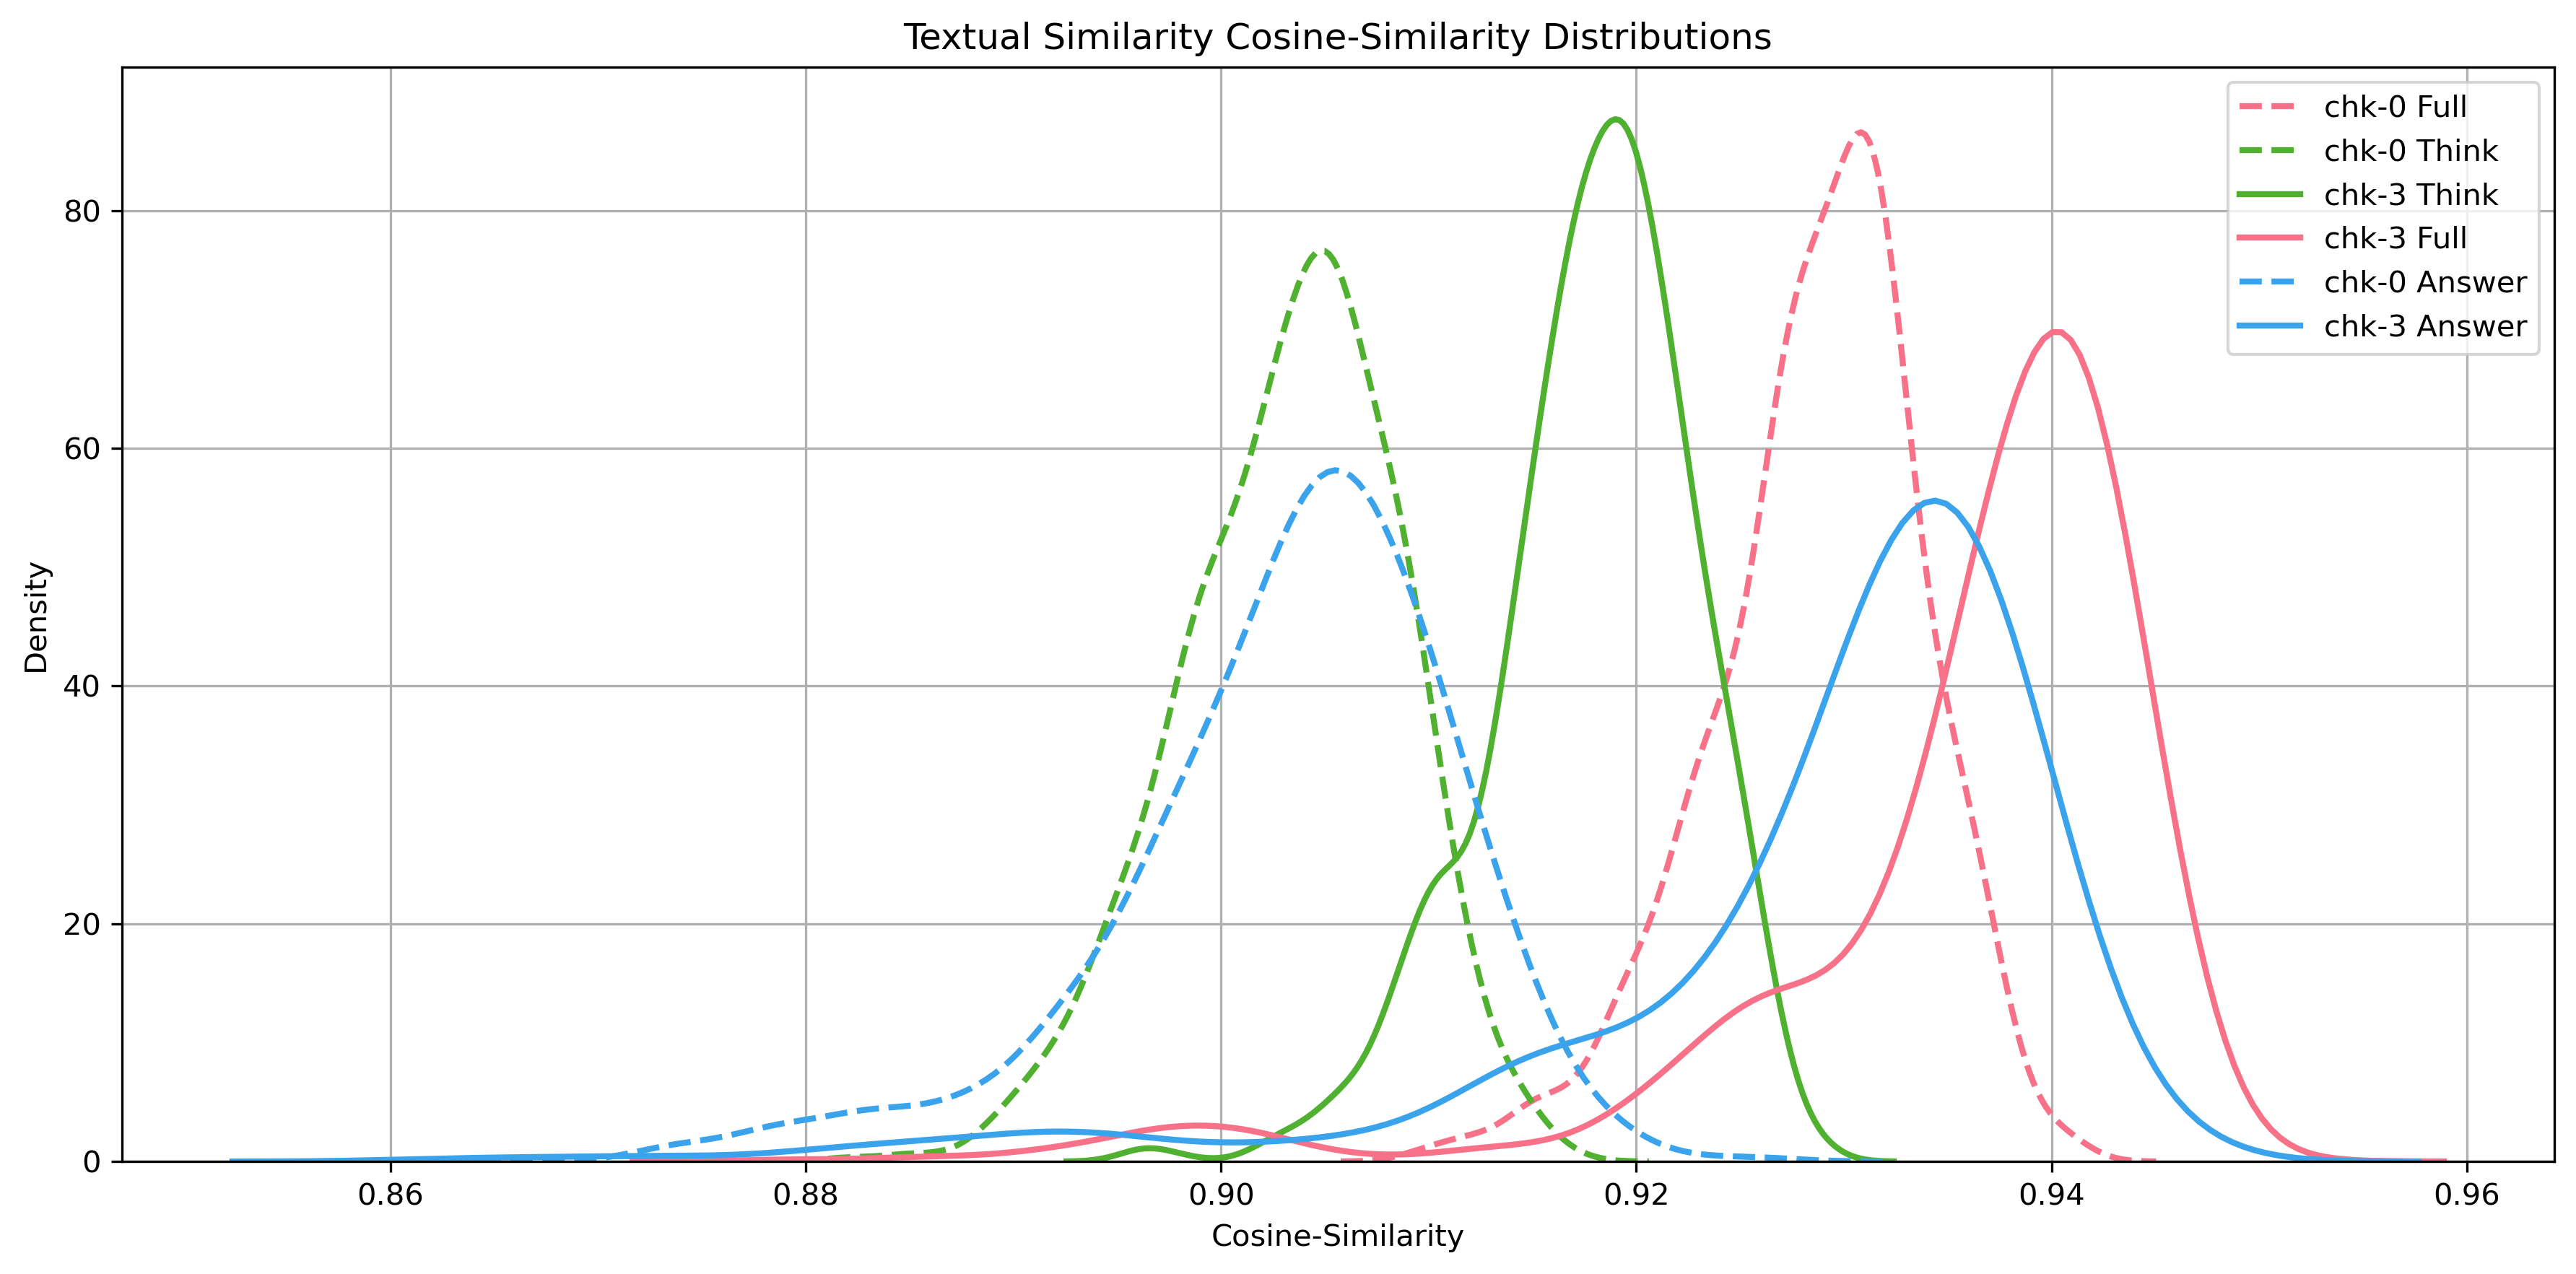
\includegraphics[width=\linewidth]{stage2_eval_figures/stage2_Cosine-Similarity_distribution.png}
        \caption{Legacy Descriptive Cosine-Similarity Distribution}
        \label{fig:ch2:stage2-cos}
    \end{minipage}
    \hfill
    \begin{minipage}[t]{0.48\textwidth}
        \centering
        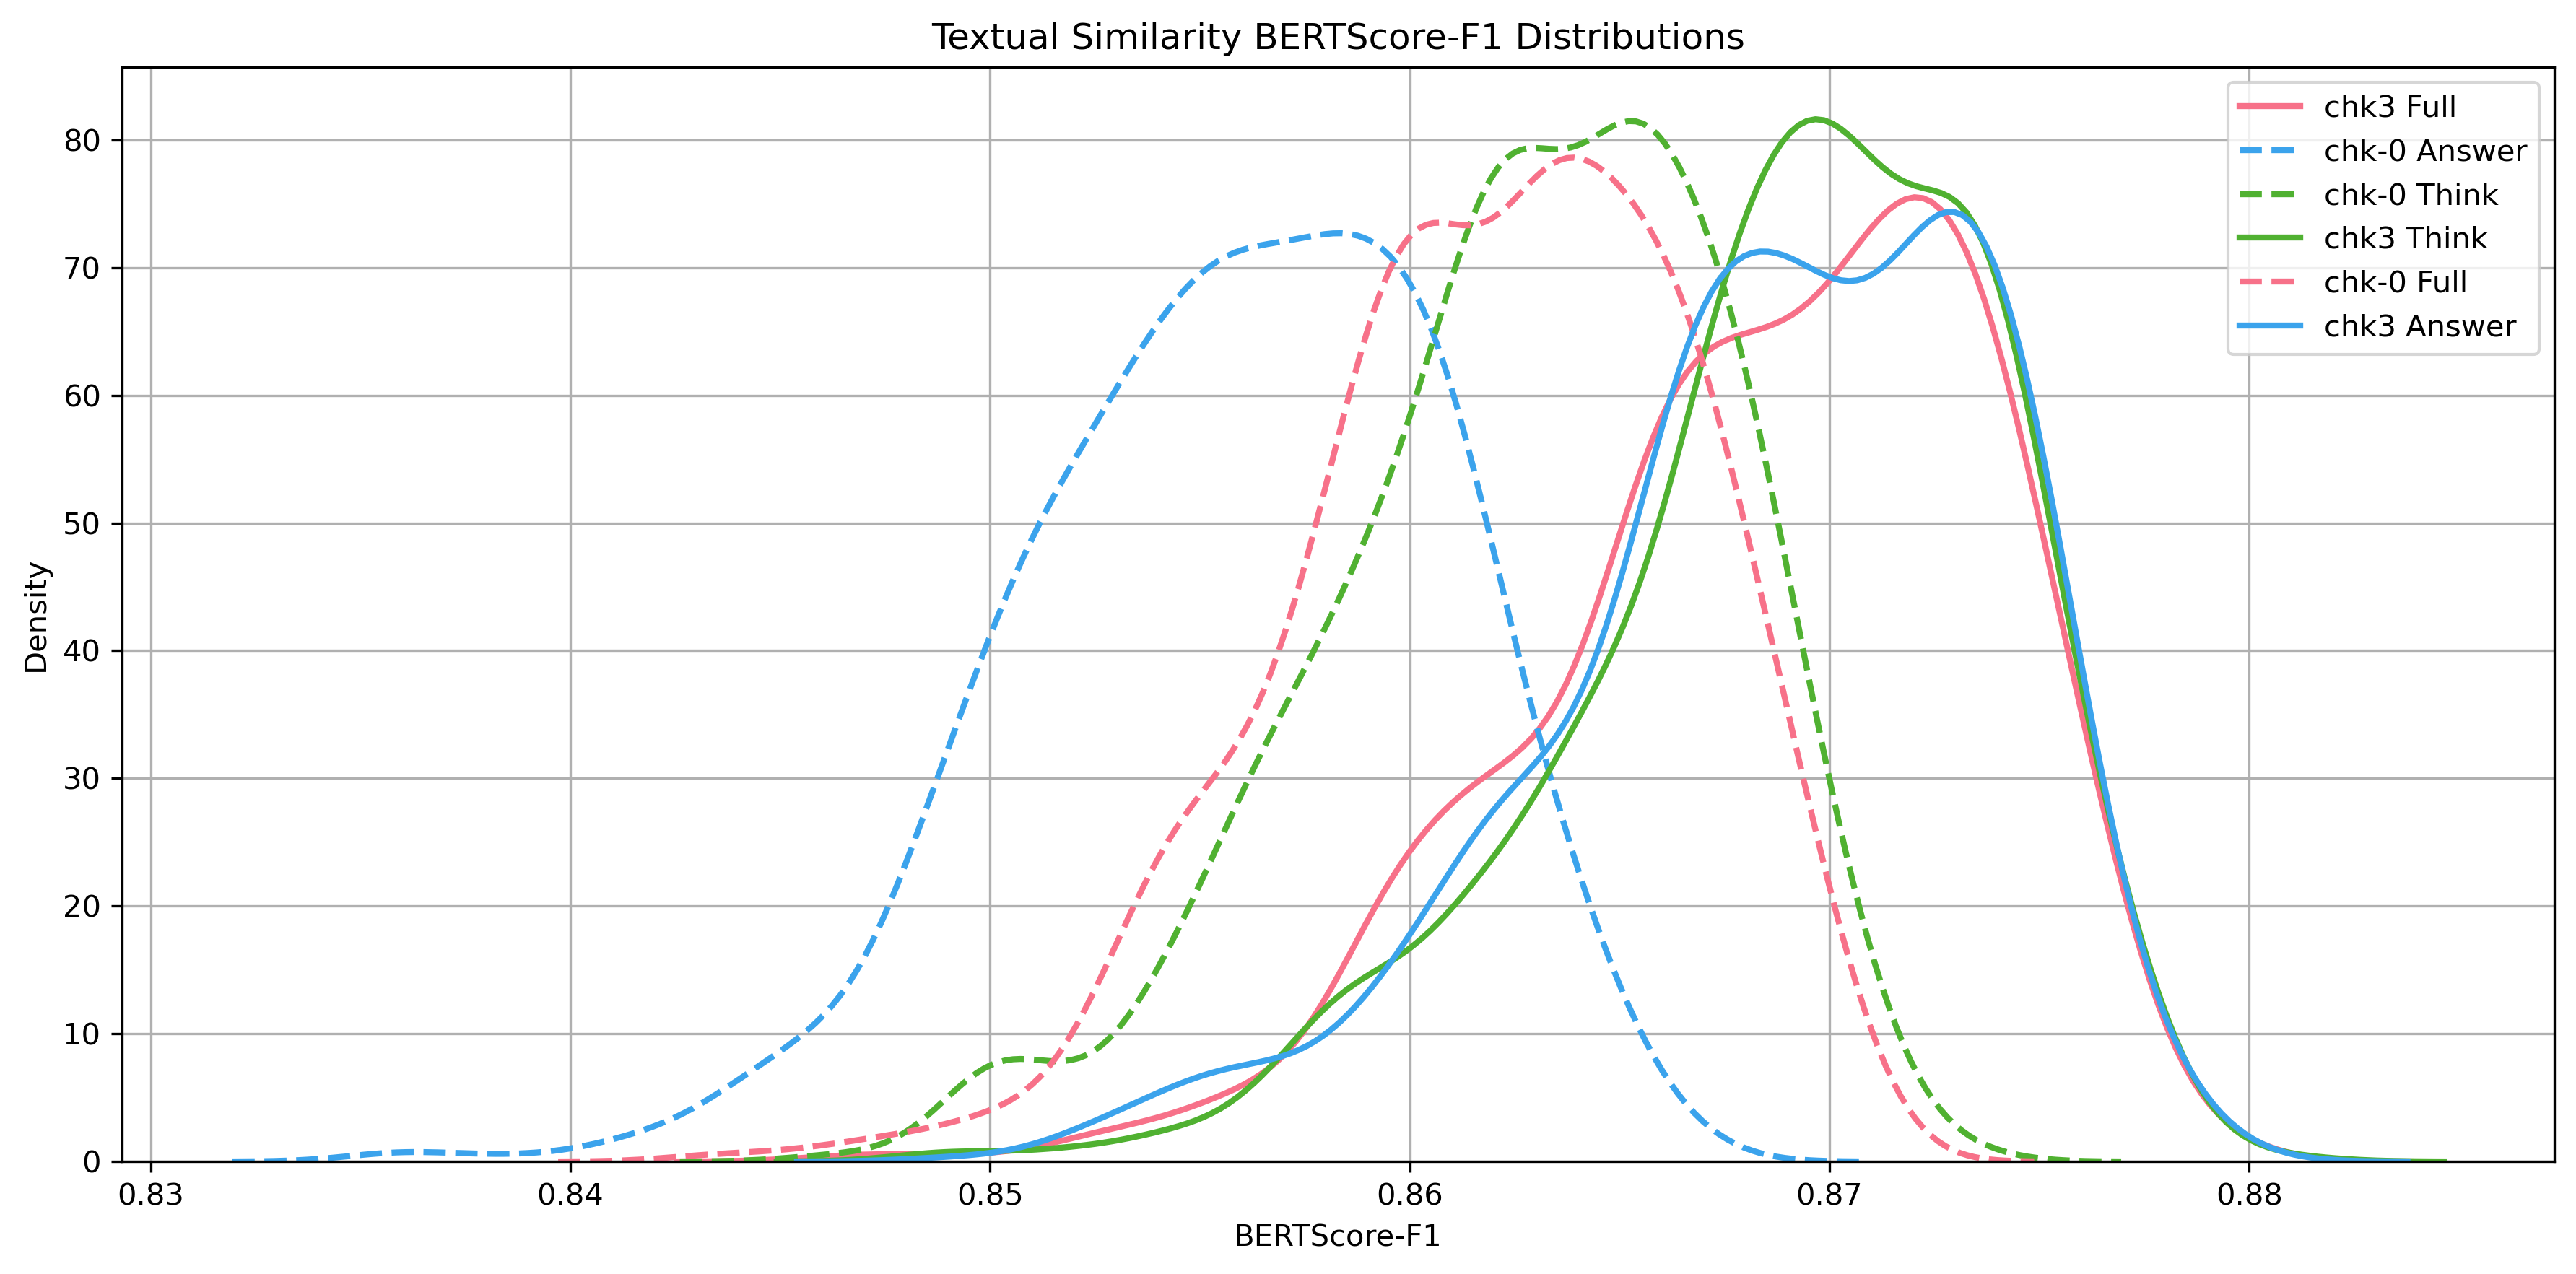
\includegraphics[width=\linewidth]{stage2_eval_figures/stage2_BERTScore-F1_distribution.png}
        \caption{Legacy Descriptive BERTScore-F1 Distribution}
        \label{fig:ch2:stage2-f1}
    \end{minipage}
\end{figure}

\begin{figure}[htp]
    \centering
    \begin{minipage}[t]{0.48\textwidth}
        \centering
        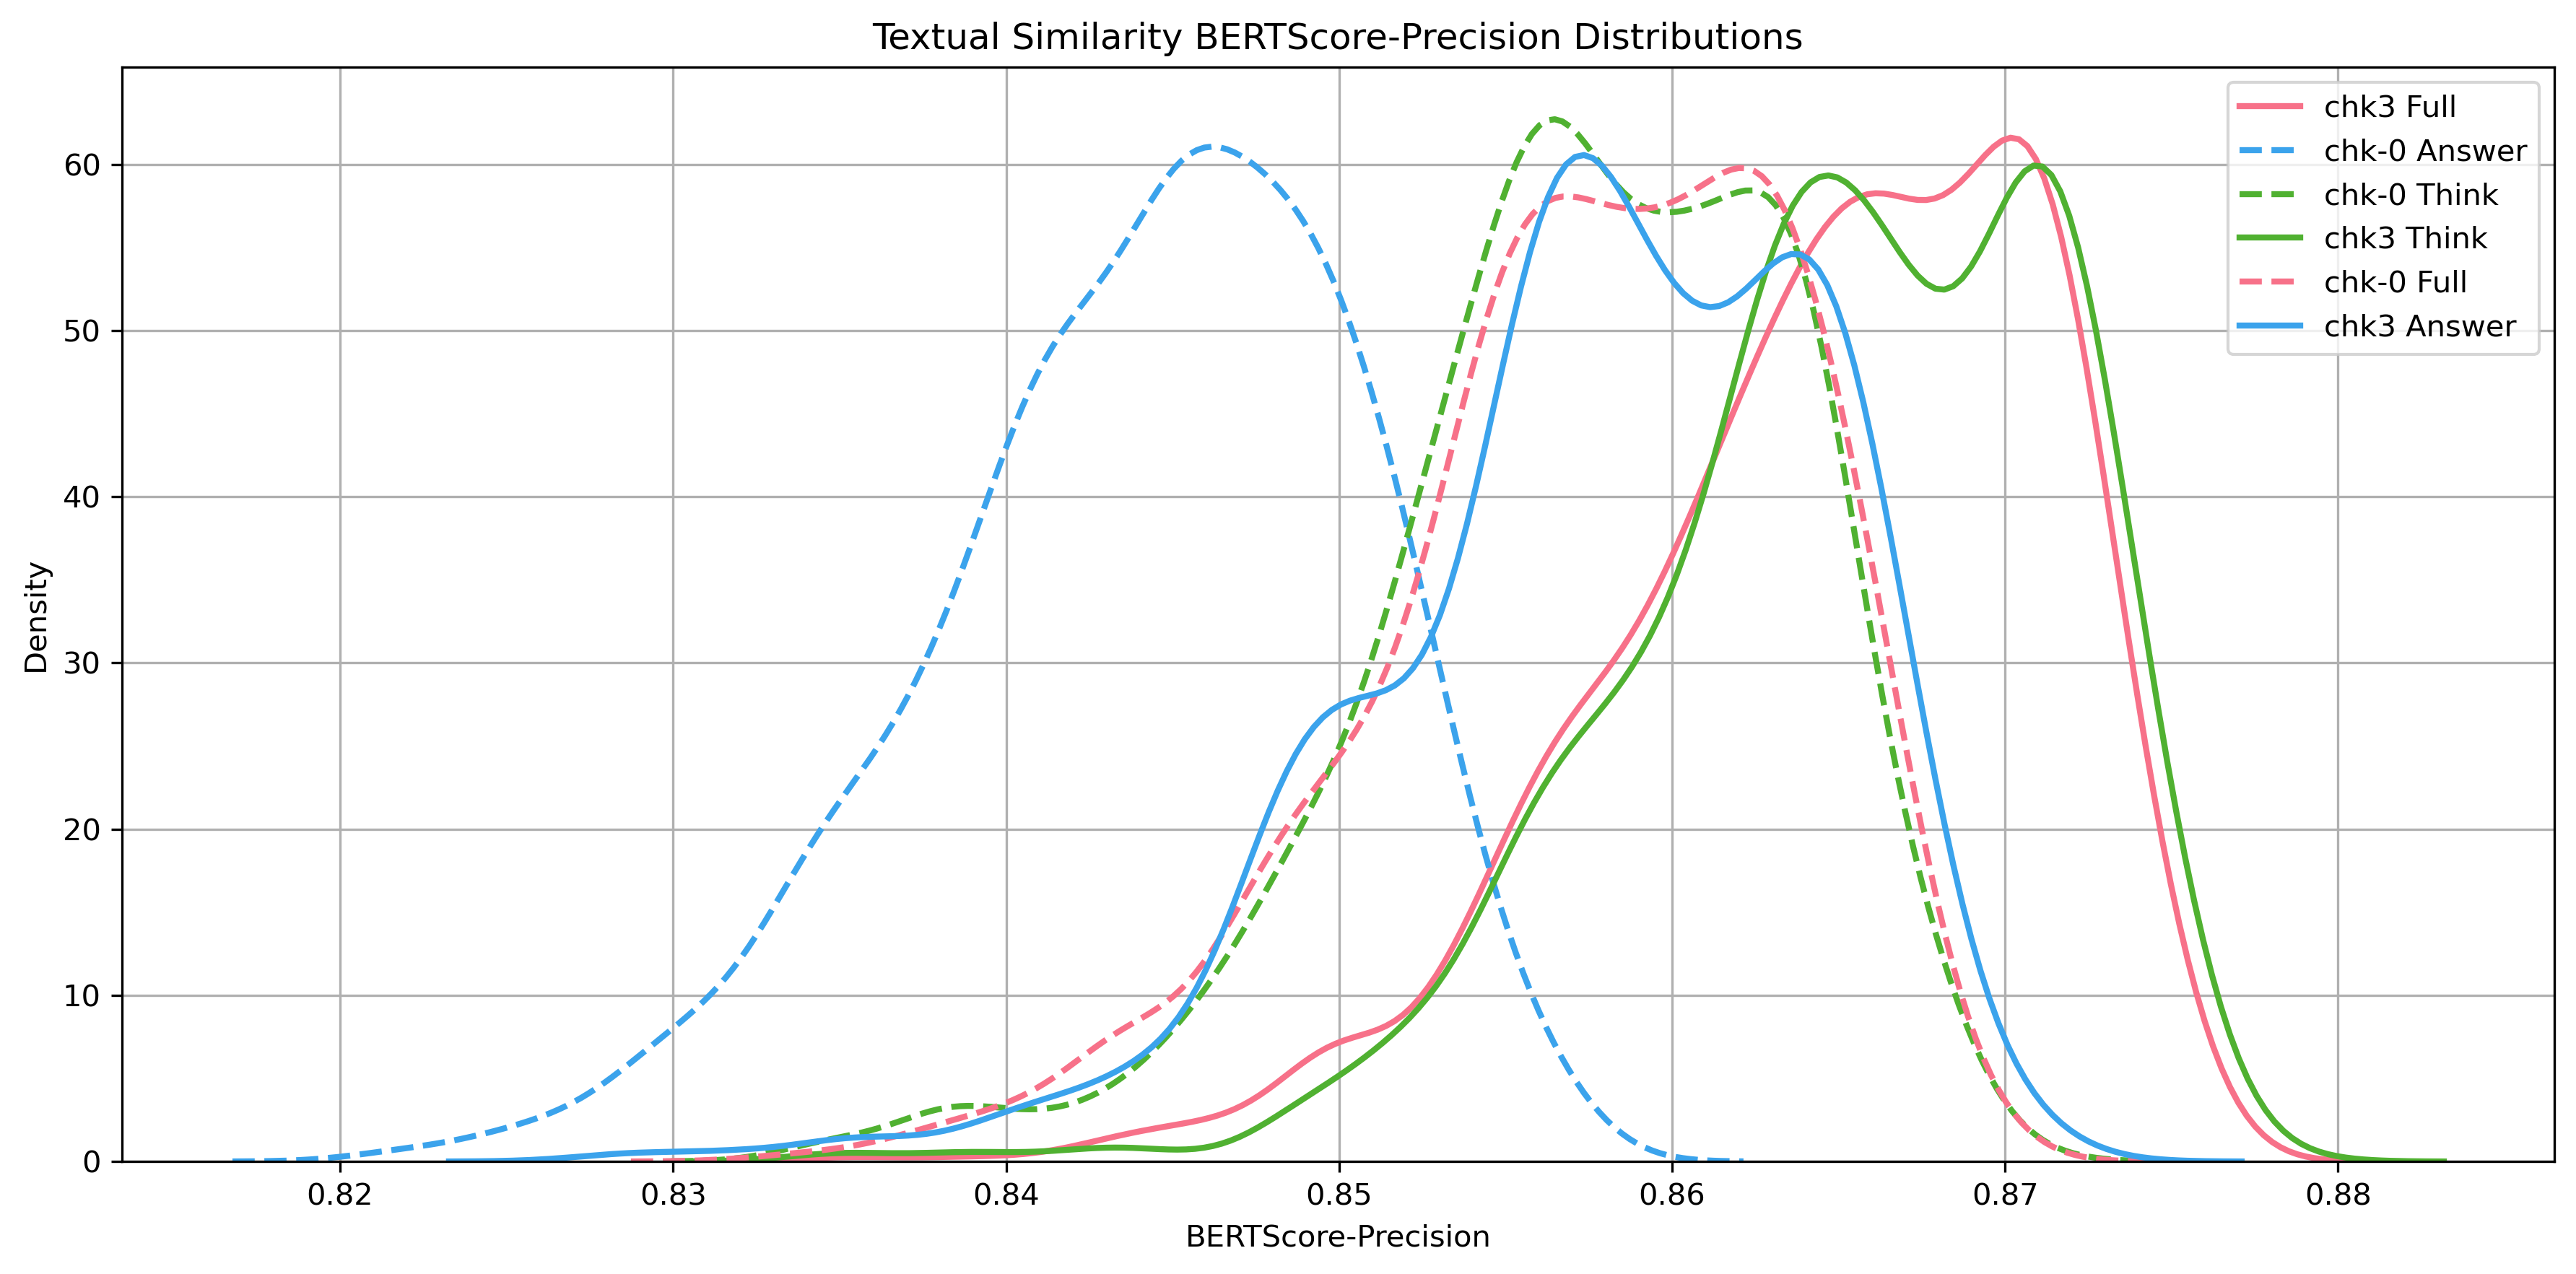
\includegraphics[width=\linewidth]{stage2_eval_figures/stage2_BERTScore-Precision_distribution.png}
        \caption{Legacy Descriptive BERTScore-Precision Distribution}
        \label{fig:ch2:stage2-precision}
    \end{minipage}
    \hfill
    \begin{minipage}[t]{0.48\textwidth}
        \centering
        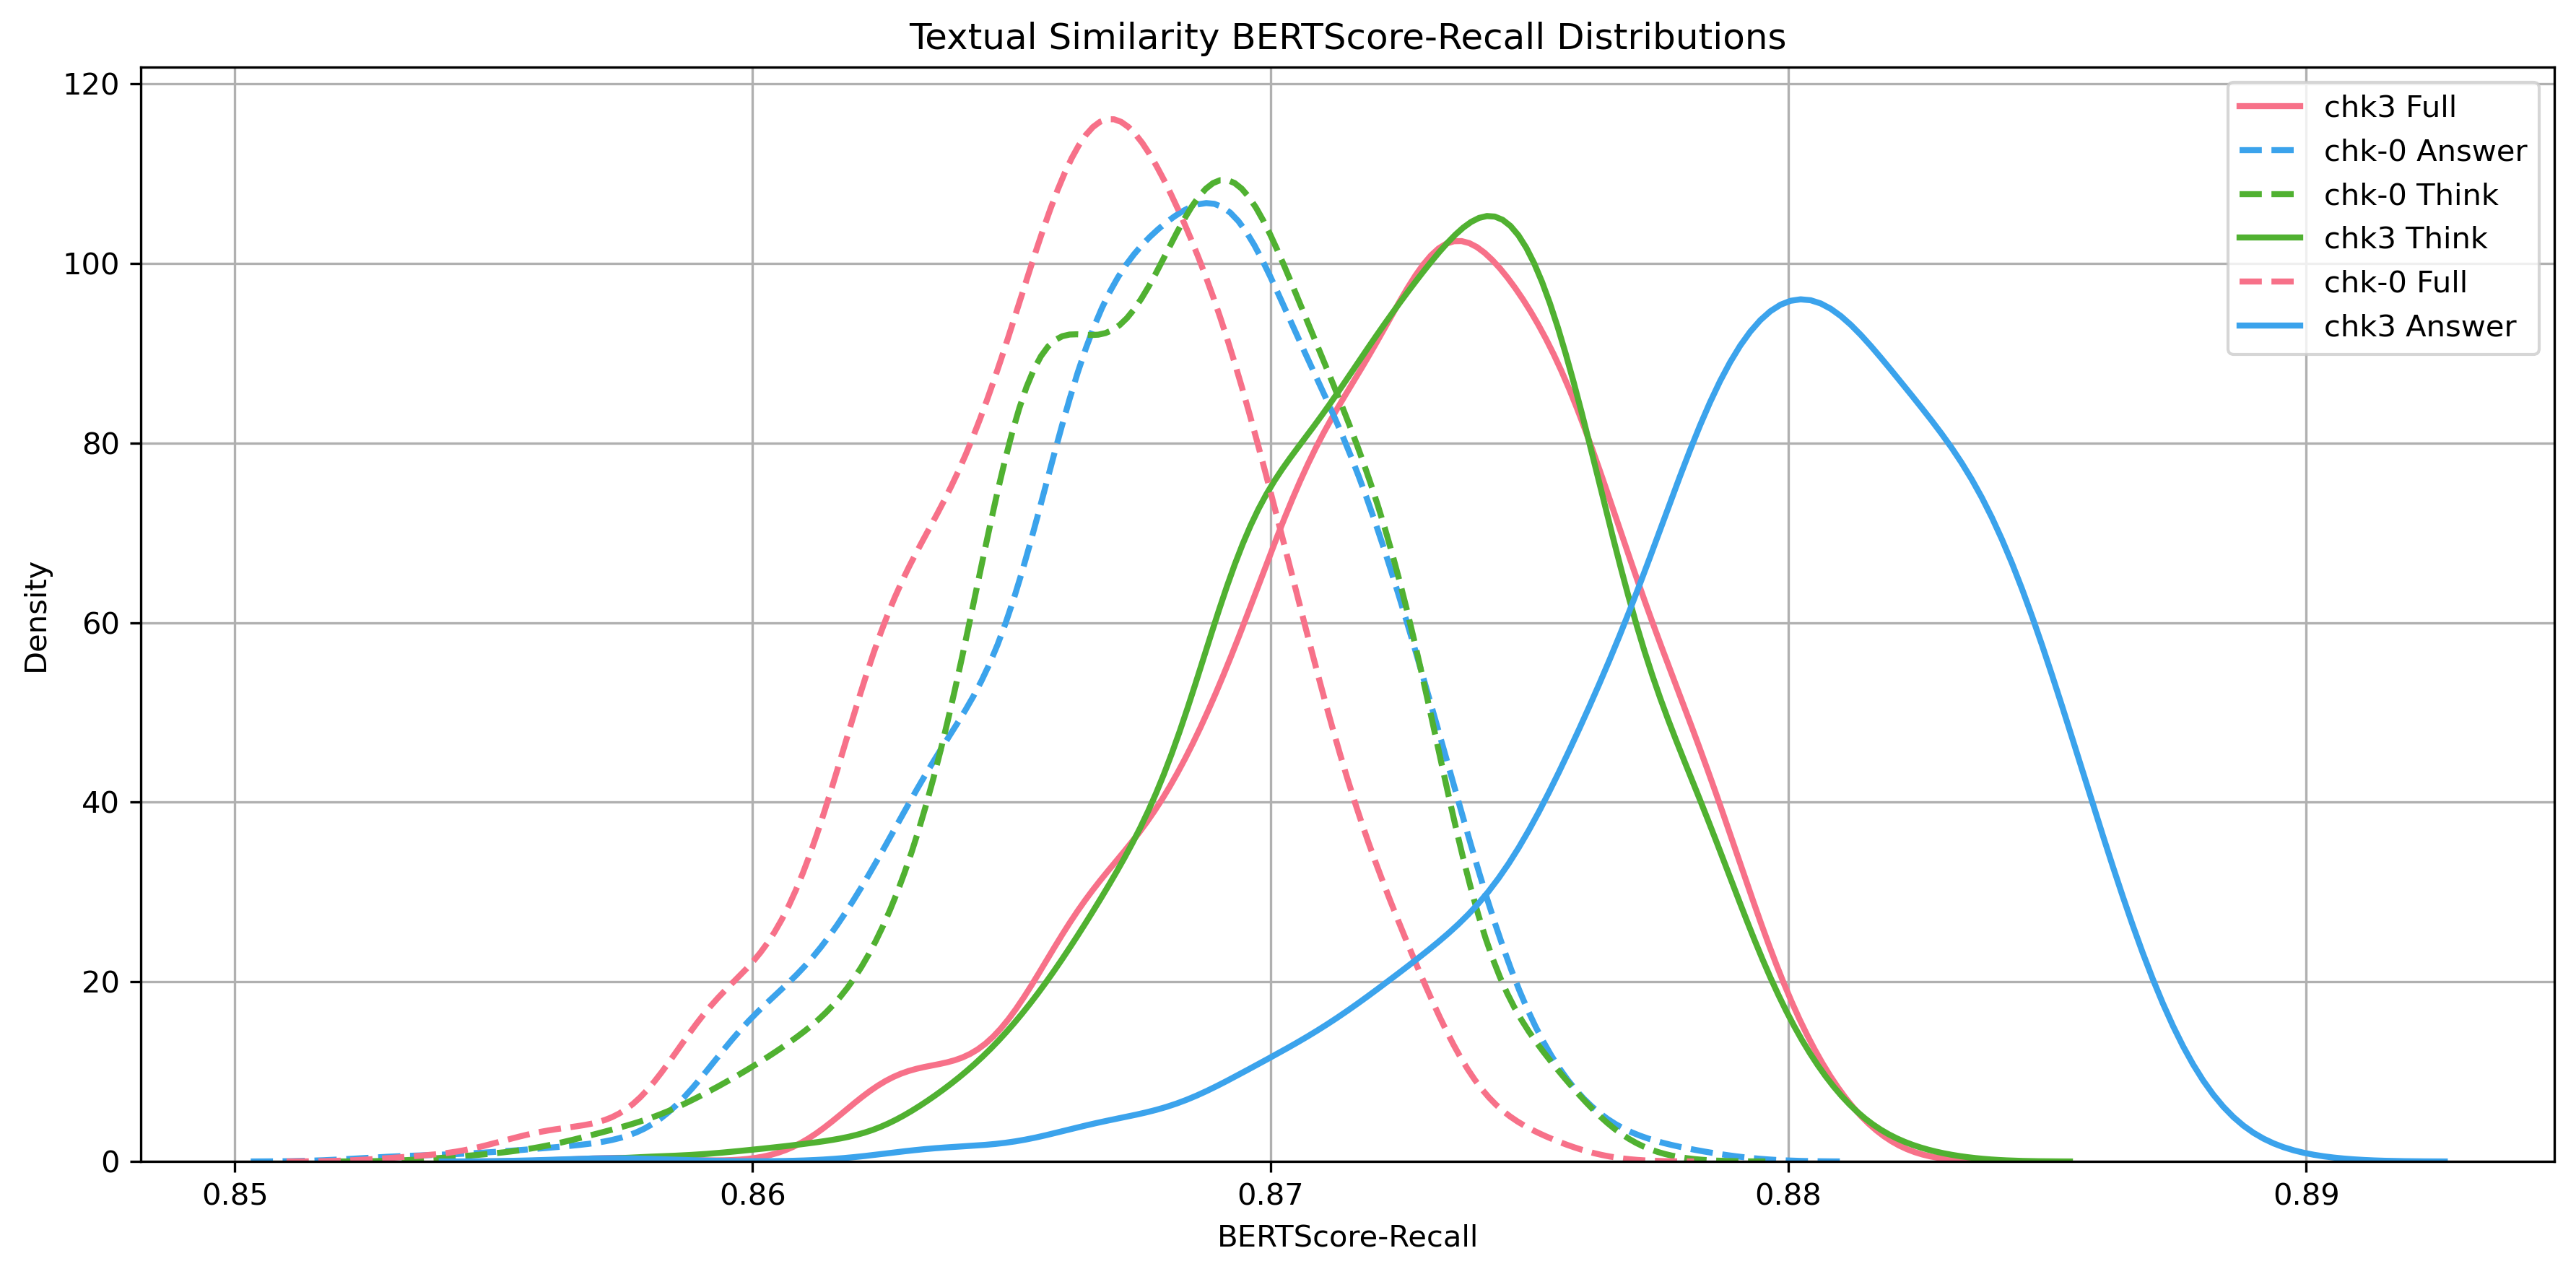
\includegraphics[width=\linewidth]{stage2_eval_figures/stage2_BERTScore-Recall_distribution.png}
        \caption{Legacy Descriptive BERTScore-Recall Distribution}
        \label{fig:ch2:stage2-recall}
    \end{minipage}
\end{figure}






\begin{table}[htp]
    \centering
    \footnotesize
    \begin{tabular}{l c c c}
        \toprule
        & \makecell[c]{Legacy Minutes\\branch}& \textit{Model chk-0}& \makecell[c]{Archived relative\\difference (in \%)}\\
        \hline
        $Cos_{full}$&0.9357&0.9287&0.7575\\ 
        $Cos_{think}$&0.9178&0.9033&1.617\\ 
        $Cos_{answer}$&0.929&0.9031&\textbf{2.872}\\ 
        \hline
        $BERTScore_{full}^{Precision}$&0.8647&0.8575&0.8441\\ 
        $BERTScore_{think}^{Precision}$&0.8653&0.8574&0.917\\ 
        $BERTScore_{answer}^{Precision}$&0.8579&0.8441&\textbf{1.6387}\\ 

        \hline
        $BERTScore_{full}^{Recall}$&0.8728&0.8664&0.7372\\ 
        $BERTScore_{think}^{Recall}$&0.8728&0.8681&0.5398\\ 
        $BERTScore_{answer}^{Recall}$&0.8796&0.868&\textbf{1.3372}\\ 

        \hline
        $BERTScore_{full}^{F1}$&0.8686&0.862&0.7673\\ 
        $BERTScore_{think}^{F1}$&0.8691&0.8628&0.735\\ 
        $BERTScore_{answer}^{F1}$&0.8688&0.8558&1.5207\\ 
        \bottomrule
    \end{tabular}
    \caption{Legacy Descriptive Text-Similarity Aggregates. The row-level scores, exact test manifest, and immutable Minutes-branch checkpoint were not recovered; no significance test or staged-training effect is claimed.}
    \label{tab:ch2:result_cos_stage2_synthetic}
\end{table}


In summary, the legacy aggregates suggest higher semantic resemblance to the reference text for the archived Minutes branch than for the base-model output under that historical evaluation. They do not establish analytical-reasoning quality, structural or factual fidelity, correct numerical and directional content, or the incremental contribution of any particular training stage.



%%%% end of textual similarity result

\fi
\subsubsection*{Target-relative Indicator Sensitivity Results}

This section reports two surviving legacy applications of the Leave-one-out
test in Eq.~\ref{eq:ch2:loo_delta}. When the archived target is the unmasked
generated Minutes, the result is an internal output-sensitivity diagnostic.
When the archived target is the actual FOMC Minutes, the result is a separate
historical external-alignment diagnostic. Neither workbook implements the
canonical synthetic-target Core8 contract defined above.



In the canonical design, for each indicator $p_i$, we generate once with the
full prompt $\mathcal{P}$ and once under the registered intervention, pairing
the same generation replicate and holding the deterministic synthetic target
fixed. The historical aggregates below do not retain row-level seeds, so their
pairing cannot be re-audited. For the unmasked-output legacy target, a positive
$\Delta_i$ measures displacement from the full output and does not imply
improvement. For the actual-Minutes legacy target, a positive $\Delta_i$ means
that removal reduces alignment to the historical Minutes, whereas a negative
value means that the masked output is more aligned.

We first use the synthetic Minutes generated from the unmasked prompt as the
target. Because this target is model-generated, the resulting scores describe
internal output sensitivity rather than validation against the historical
Minutes. The surviving workbook permits recovery of the historical aggregate
point estimates, reported in
Table~\ref{tab:ch2:loo_internal_legacy}. The original row-level generations,
meeting identifiers, and seed metadata for this 25-indicator experiment are
unavailable; consequently, the historical significance stars are not
retained and no clustered inferential claim is made from this table. A
separate seven-indicator pilot survives at row level, but its indicator and
section populations do not match this table, its decoding was unseeded, and
its masking operation also rewrote the prompt template. It is therefore
excluded from the Chapter 2 results.

\begin{table}[htbp]
\centering
\scriptsize
\begin{threeparttable}
\begin{tabular}{p{4.7cm}ccc}
\toprule
\textbf{Indicator} & \textbf{Participants' Views} & \textbf{Economic Situation} & \textbf{Financial Situation} \\
\midrule
Bank Capital & $+0.2164$ & $+0.2054$ & $+0.2168$ \\
Bank Credit to Private Sector & $+0.2067$ & $+0.2119$ & $+0.2183$ \\
Business Investment & $+0.2121$ & $+0.2162$ & $+0.2094$ \\
Commodity Prices & $+0.2093$ & $+0.2121$ & $+0.2194$ \\
Consumer Confidence Index & $+0.1567$ & $+0.1646$ & $+0.1669$ \\
Consumer Price Index (CPI) & $+0.2081$ & $+0.2153$ & $+0.2152$ \\
Equity Market Indices & $+0.2102$ & $+0.2088$ & $+0.2137$ \\
Exchange Rate & $+0.2079$ & $+0.2119$ & $+0.2173$ \\
Federal Funds Rate & $+0.2063$ & $+0.2144$ & $+0.2176$ \\
Federal Reserve Balance Sheet & $+0.2096$ & $+0.2120$ & $+0.2198$ \\
GDP Growth & $+0.2093$ & $+0.2100$ & $+0.2131$ \\
Government Purchases & $+0.2103$ & $+0.2081$ & $+0.2096$ \\
Home Prices & $+0.2063$ & $+0.2143$ & $+0.2178$ \\
Housing Starts & $+0.2043$ & $+0.2054$ & $+0.2133$ \\
Industrial Production & $+0.2110$ & $+0.2132$ & $+0.2212$ \\
International Equity Markets & $+0.2080$ & $+0.2091$ & $+0.2136$ \\
Labour Market & $+0.2323$ & $+0.2336$ & $+0.2380$ \\
Market Volatility (VIX) & $+0.2067$ & $+0.2082$ & $+0.2236$ \\
Money Supply & $+0.1990$ & $+0.2066$ & $+0.2045$ \\
Mortgage Rates & $+0.2039$ & $+0.2074$ & $+0.2080$ \\
Overnight Rate & $+0.2057$ & $+0.2082$ & $+0.2094$ \\
Personal Consumption Expenditures (PCE) & $+0.2097$ & $+0.2084$ & $+0.2154$ \\
Trade Balance & $+0.2070$ & $+0.2065$ & $+0.2136$ \\
Treasury Yields & $+0.2058$ & $+0.2136$ & $+0.2145$ \\
Unemployment Rate & $+0.2045$ & $+0.2098$ & $+0.2125$ \\
\bottomrule
\end{tabular}

\begin{tablenotes}[flushleft]
\footnotesize
\item \textit{Notes:} Entries are historical descriptive means of
$\Delta_i=1-\operatorname{Cos}(o_{\mathrm{masked},i},o_{\mathrm{full}})$.
They measure internal output sensitivity. The table is regenerated from the
surviving aggregate workbook; significance markers are omitted because
meeting-clustered uncertainty cannot be reconstructed without row-level data.
The surviving internal workbook contains 25 indicators and omits
Corporate Bond Yields; historical cell sizes vary from 897 to 1,337 pairs.
\end{tablenotes}
\caption{Legacy Descriptive Leave-One-Out Output Sensitivity (Target: Unmasked Generated Minutes)}
\label{tab:ch2:loo_internal_legacy}
\end{threeparttable}
\end{table}


We next use the corresponding historical FOMC Minutes section as the fixed
target. The primary quantity is the raw signed delta in
Eq.~\ref{eq:ch2:loo_delta}, not the masked output's absolute distance and not a
percentage of that distance. The surviving aggregate workbook stores
indicator-specific paired means, so its point estimate can be recovered
algebraically as
$\bar{\Delta}_i=\bar{d}_{\mathrm{masked},i}-\bar{d}_{\mathrm{full},i}$.
Table~\ref{tab:ch2:loo_external_legacy} reports this descriptive recovery.
The underlying row-level generations for this 26-indicator experiment no
longer survive, so the historical standard errors cannot be re-clustered by
meeting; the table intentionally contains no significance stars or
inferential claims.

\begin{table}[htbp]
\centering
\scriptsize
\begin{threeparttable}
\begin{tabular}{p{4.7cm}ccc}
\toprule
\textbf{Indicator} & \textbf{Participants' Views} & \textbf{Economic Situation} & \textbf{Financial Situation} \\
\midrule
Bank Capital & $+0.0024$ & $0.0000$ & $0.0000$ \\
Bank Credit to Private Sector & $+0.0021$ & $+0.0014$ & $+0.0188$ \\
Business Investment & $+0.0061$ & $+0.0083$ & $+0.0030$ \\
Commodity Prices & $-0.0025$ & $+0.0006$ & $+0.0026$ \\
Consumer Confidence Index & $+0.0011$ & $+0.0015$ & $+0.0021$ \\
Consumer Price Index (CPI) & $+0.0033$ & $+0.0059$ & $+0.0022$ \\
Corporate Bond Yields & $+0.0006$ & $+0.0004$ & $-0.0007$ \\
Equity Market Indices & $+0.0018$ & $+0.0013$ & $-0.0007$ \\
Exchange Rate & $+0.0018$ & $+0.0043$ & $+0.0011$ \\
Federal Funds Rate & $+0.0044$ & $+0.0008$ & $+0.0006$ \\
Federal Reserve Balance Sheet & $-0.0005$ & $+0.0017$ & $+0.0020$ \\
GDP Growth & $+0.0093$ & $+0.0087$ & $+0.0028$ \\
Government Purchases & $-0.0001$ & $-0.0015$ & $+0.0014$ \\
Home Prices & $+0.0027$ & $-0.0002$ & $+0.0024$ \\
Housing Starts & $+0.0040$ & $-0.0011$ & $+0.0021$ \\
Industrial Production & $+0.0033$ & $+0.0003$ & $+0.0017$ \\
International Equity Markets & $+0.0035$ & $+0.0001$ & $+0.0004$ \\
Labour Market & $+0.0241$ & $+0.0250$ & $+0.0262$ \\
Market Volatility (VIX) & $-0.0004$ & $+0.0028$ & $-0.0005$ \\
Money Supply & $+0.0007$ & $+0.0004$ & $0.0000$ \\
Mortgage Rates & $+0.0017$ & $+0.0009$ & $+0.0038$ \\
Overnight Rate & $+0.0009$ & $+0.0035$ & $-0.0003$ \\
Personal Consumption Expenditures (PCE) & $-0.0079$ & $+0.0020$ & $+0.0030$ \\
Trade Balance & $+0.0022$ & $+0.0054$ & $+0.0024$ \\
Treasury Yields & $+0.0015$ & $+0.0015$ & $+0.0014$ \\
Unemployment Rate & $+0.0040$ & $+0.0020$ & $+0.0009$ \\
\bottomrule
\end{tabular}

\begin{tablenotes}[flushleft]
\footnotesize
\item \textit{Notes:} Entries are signed raw cosine-similarity deltas,
$\bar{\Delta}_i=\bar{s}_{\mathrm{full}}-\bar{s}_{\mathrm{masked},i}$.
Positive values mean that masking reduces alignment with the historical
Minutes; negative values mean that masking improves alignment. Values are
descriptive recoveries from the surviving paired aggregate workbook.
Row-level outputs, meeting clusters, and seed metadata are unavailable, so
confidence intervals and significance stars are deliberately omitted.
The surviving external workbook contains 26 indicators, and historical cell
sizes vary from 897 to 1,337 pairs; comparisons across cells are therefore
descriptive rather than estimates on a common balanced sample.
\end{tablenotes}
\caption{Legacy Descriptive Signed Leave-One-Out Delta against Actual FOMC Minutes}
\label{tab:ch2:loo_external_legacy}
\end{threeparttable}
\end{table}

Taken descriptively, the recovered results are heterogeneous and
section-dependent. Labour-market masking produces the largest positive delta
in all three sections (approximately 0.024--0.026), whereas several cells are
near zero or negative; for example, PCE has a negative delta in Participants'
Views. These patterns are consistent with indicator-specific sensitivity, but
they are not promoted to current statistical evidence. The canonical paired
pipeline must be rerun from reconstructed prompts and a newly versioned,
hash-frozen actual-Minutes reference before meeting-clustered confidence
intervals or adjusted significance are reported. That canonical rerun must use
the frozen deterministic synthetic source-grounded target. Separately, the
actual-Minutes source family underlying the legacy external workbook has been
recovered and cross-validated against 3,481 surviving records, but the exact
historical row manifest and full/masked generations remain unavailable.








\subsubsection*{Legacy Exploratory Association Results}

The archived analysis applied the sentiment--return regression in Eq.~\ref{eq:ch2:sentiment_reg} (\citet{tadle2022fomc}) to synthetic Minutes and to a base-model series. Figure~\ref{fig:ch2:bootstrap_ft_base} is retained as a legacy record of the resulting bootstrapped $\beta_{Z_m}$ and $t$-statistic distributions. The exact source series, immutable Minutes-branch checkpoint, resampling unit, and model-difference test were not recovered, so this figure is not treated as a verified main result.


\begin{figure}[htbp]
    \centering
    %----------------- FT -----------------%
    \begin{subfigure}[t]{0.48\textwidth}
        \centering
        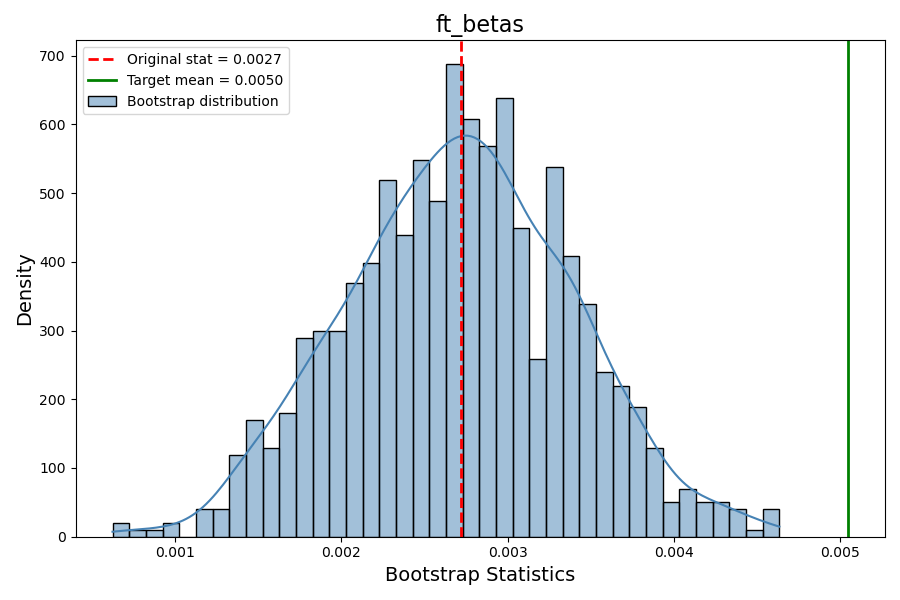
\includegraphics[width=\textwidth]{simulation_figure/ft_betas.png}
        \caption{Legacy Minutes branch: coefficient distribution}
    \end{subfigure}
    \hfill
    \begin{subfigure}[t]{0.48\textwidth}
        \centering
        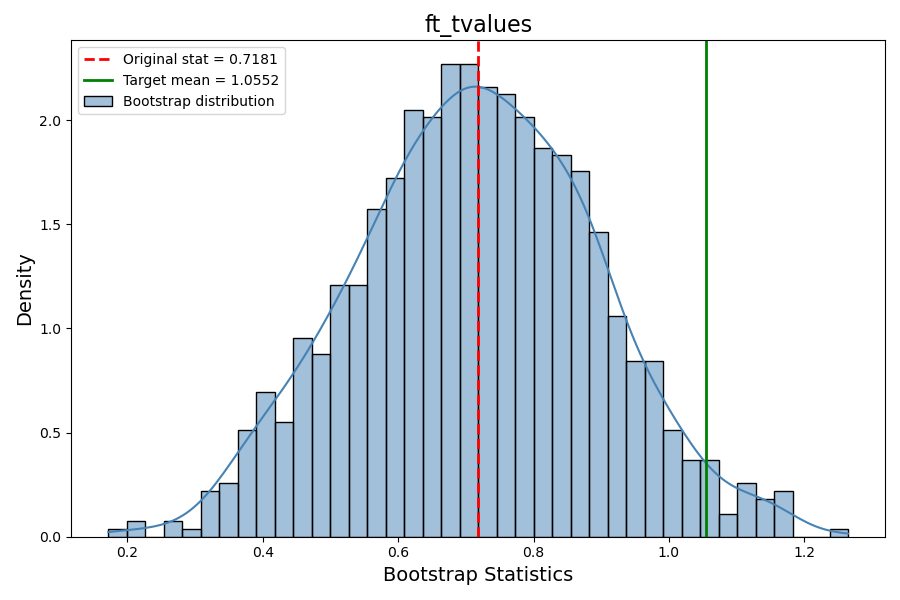
\includegraphics[width=\textwidth]{simulation_figure/ft_tvalues.png}
        \caption{Legacy Minutes branch: t-statistic distribution}
    \end{subfigure}
    \vspace{0.8em}

    %----------------- Base -----------------%
    \begin{subfigure}[t]{0.48\textwidth}
        \centering
        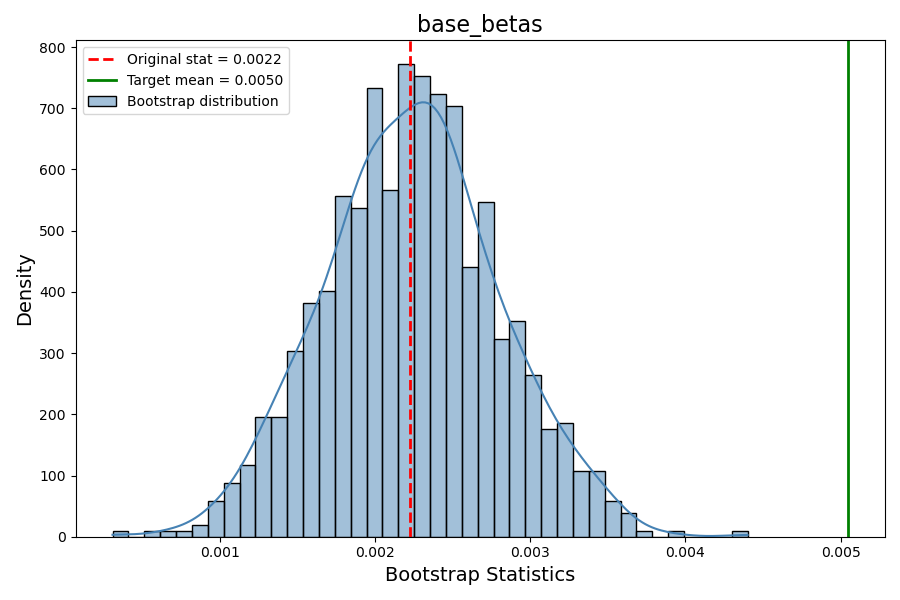
\includegraphics[width=\textwidth]{simulation_figure/base_betas.png}
        \caption{\textit{Model chk-0}: coefficient distribution}
    \end{subfigure}
    \hfill
    \begin{subfigure}[t]{0.48\textwidth}
        \centering
        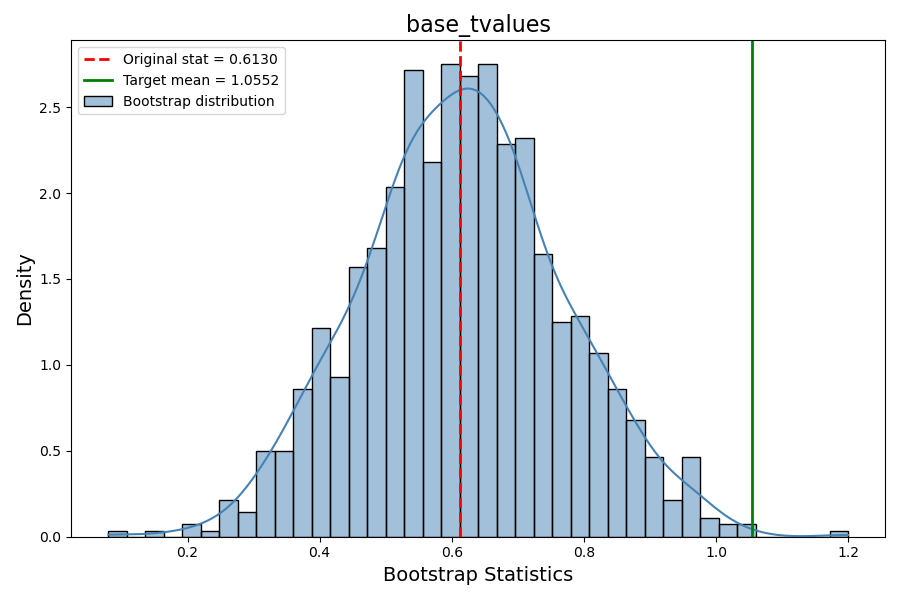
\includegraphics[width=\textwidth]{simulation_figure/base_tvalues.png}
        \caption{\textit{Model chk-0}: t-statistics distribution}
    \end{subfigure}
    \caption{Legacy, unverified bootstrap distributions of $Z_{t}^{M}$ coefficients and t-statistics for the archived Minutes branch and \textit{Model chk-0}.}
    \label{fig:ch2:bootstrap_ft_base}
\end{figure}

% coefficient
% base: 0.0022399151956866616, ft:0.0027096296763361653
% target: 0.005048811

% t-statistics
% base: 0.6168947613082458, ft: 0.7152094287360642
% target: -0.289101766
% 

The archived coefficient and $t$-statistic summaries are not sufficient to test equality with a benchmark or a difference between models. Accordingly, the earlier ``gap reduction'' interpretation is not used as a chapter-level finding. At most, the figure documents the direction of a legacy exploratory association; it provides no causal evidence of market impact and no verified incremental effect attributable to the paper-level \textit{Model chk-2}.





% policy-decision branch

\subsubsection*{Policy-Decision Branch Performance}

The principal quality check uses the 13-meeting test split that was excluded
from decision SFT and GRPO training. Table~\ref{tab:ch2:decision_test_n13}
compares the three model states on identical meetings and retains invalid
outputs in every denominator.

\begin{table}[htbp]
    \centering
    \footnotesize
    \setlength{\tabcolsep}{4pt}
    \begin{tabularx}{\textwidth}{@{}>{\raggedright\arraybackslash}Xccccc@{}}
        \toprule
        \textbf{Model or state} & \textbf{Direction} &
        \makecell{\textbf{Balanced}\\\textbf{accuracy}} &
        \textbf{Macro F1} & \makecell{\textbf{Exact}\\\textbf{action}} &
        \textbf{Delivery} \\
        \midrule
        \textit{Model chk-1} cp200 & 5/13 (38.46\%) & 18.52\% & 19.61\% & 5/13 (38.46\%) & 0/13 \\
        \textit{Model chk-3}, SFT cp38 & 4/13 (30.77\%) & 44.44\% & 30.00\% & 4/13 (30.77\%) & 0/13 \\
        \textit{Model chk-3}, GRPO cp450 & 4/13 (30.77\%) & 44.44\% & 28.72\% & 4/13 (30.77\%) & 0/13 \\
        \bottomrule
    \end{tabularx}
    \caption{Training-Held-Out Decision Results (13 Meetings). Direction and exact-action accuracy retain invalid responses in the denominator; balanced accuracy and macro F1 use the fixed three-class definition. Checkpoint 38 is the pre-GRPO SFT state of \textit{Model chk-3}; checkpoint 450 is its evaluated post-GRPO state.}
    \label{tab:ch2:decision_test_n13}
\end{table}

The test population contains three cuts, nine holds, and one hike. All three
models have zero recall on the cut meetings, and none produces a delivery-valid
response. The higher ordinary accuracy of \textit{Model chk-1} reflects five
correct holds rather than broader class coverage; its balanced accuracy is the
lowest of the three. SFT checkpoint 38 and GRPO checkpoint 450 tie on direction
accuracy, balanced accuracy, and exact-action accuracy, while SFT has the
slightly higher macro F1. Thus the test provides no observed GRPO gain in
decision quality or delivery. Although this split was excluded from training,
it contains only 13 meetings and has already been opened; it is not a new
prospective validation sample and supports no promotion claim.

\paragraph*{Within-release diagnostic.}
Table~\ref{tab:ch2:decision_all237} reports the secondary comparison over all
237 unique meetings. Because 211 observations are training meetings, these
figures characterize behaviour on the frozen release rather than
generalization.

\begin{table}[htbp]
    \centering
    \footnotesize
    \setlength{\tabcolsep}{4pt}
    \begin{tabularx}{\textwidth}{@{}>{\raggedright\arraybackslash}Xccccc@{}}
        \toprule
        \textbf{Model or baseline} & \makecell{\textbf{Direction}\\\textbf{accuracy}} &
        \makecell{\textbf{Balanced}\\\textbf{accuracy}} &
        \textbf{Macro F1} & \makecell{\textbf{Exact-action}\\\textbf{accuracy}} &
        \makecell{\textbf{Delivery}\\\textbf{valid}} \\
        \midrule
        Always hold & 70.89\% & 33.33\% & 27.65\% & 70.89\% & --- \\
        \textit{Model chk-1} cp200 & 36.29\% & 20.38\% & 24.98\% & 35.44\% & 0.00\% \\
        \textit{Model chk-3}, SFT cp38 & \textbf{48.10\%} & \textbf{34.01\%} & \textbf{35.25\%} & \textbf{45.57\%} & 8.86\% \\
        \textit{Model chk-3}, GRPO cp450 & 43.04\% & 28.24\% & 29.81\% & 40.93\% & \textbf{21.52\%} \\
        \bottomrule
    \end{tabularx}
    \caption{Within-Release Decision Diagnostic (237 Meetings). The always-hold row illustrates class imbalance and has no model-output delivery measure. The table is training-dominated and is not a held-out generalization estimate.}
    \label{tab:ch2:decision_all237}
\end{table}

\begin{table}[htbp]
    \centering
    \footnotesize
    \begin{tabular}{lcc}
        \toprule
        \textbf{Metric} & \textbf{GRPO cp450 minus SFT cp38} & \textbf{Paired 95\% CI} \\
        \midrule
        Direction accuracy & $-5.06$ pp & $[-11.39,\ 1.27]$ \\
        Balanced accuracy & $-5.77$ pp & $[-11.90,\ 0.16]$ \\
        Macro F1 & $-5.45$ pp & $[-11.15,\ -0.06]$ \\
        Exact-action accuracy & $-4.64$ pp & $[-10.97,\ 1.69]$ \\
        Delivery-valid rate & $+12.66$ pp & $[7.17,\ 18.57]$ \\
        \bottomrule
    \end{tabular}
    \caption{Paired SFT-to-GRPO Contrasts in the 237-Meeting Diagnostic. Intervals use 10,000 target-direction-stratified, meeting-paired bootstrap draws.}
    \label{tab:ch2:decision_all237_contrasts}
\end{table}

Within this diagnostic, SFT checkpoint 38 has the strongest point estimate on
all four decision-quality metrics, whereas GRPO checkpoint 450 has the highest
delivery-valid rate. GRPO increases delivery by 12.66 percentage points but
reduces all four decision-quality point estimates. The macro-F1 interval lies
entirely below zero; the direction, balanced-accuracy, and exact-action
intervals cross zero. This is a format-versus-decision trade-off, not an
across-the-board GRPO improvement. Together with the small opened test split
and the null formal checkpoint selection, the evidence leaves checkpoint 450
as an exploratory evaluated state rather than a promoted model.






\section{Conclusion}\label{ch2:sec:conclusion}


In conclusion, this chapter implements a shared-parent, two-branch framework.
\textit{Model chk-0} is the pretrained starting model, and \textit{Model
chk-1} is the analytical model and common downstream parent. The Minutes
branch follows \textit{Model chk-0} $\rightarrow$ \textit{Model
chk-1} $\rightarrow$ \textit{Model chk-2}; paper-level \textit{Model chk-2} is
repository artifact \texttt{chk3} at checkpoint 318. The independent decision
branch follows \textit{Model chk-1} $\rightarrow$ \textit{Model chk-3}, where
decision SFT checkpoint 38 initializes GRPO and the best-observed exploratory
checkpoint 450 is retained only for post-GRPO evaluation under repository
artifact \texttt{chk4}; the formal selected checkpoint is null. \textit{Model
chk-3} does not consume outputs from \textit{Model chk-2}. In the completed
rewriting task, the input is a \textit{Model chk-1} analysis, and the
supervised completion contains a synthetic teacher-generated fidelity rationale
followed by a Minutes-style paragraph derived from the same analysis.  Official
FOMC Minutes are not used as the response target.

The analysis SFT stage is completed over three epochs and 255 optimization
steps, and checkpoint 200 is retained as the common downstream parent. The
Minutes-rewriting SFT stage terminates at step 318. Its checkpoint-selection
diagnostic is reported in Appendix~\ref{app:checkpoint_selection} and is not
used as the chapter's main performance evidence.

On the external 128-meeting evaluation with ten stochastic replicates per
meeting and model, \textit{Model chk-2} improves exact numeric fidelity over
\textit{Model chk-1} by 5.625 percentage points, MPNet cosine by 6.145 points,
and BERTScore F1 by 5.713 points. The paired intervals for all three differences
exclude zero after Holm correction. Structure/delivery is directionally higher
but uncertain. Date fidelity and degeneration-free delivery each have one
additional failure among 1,280 generations. Although both differences are
statistically unresolved, they trigger the preregistered zero-tolerance rule
and the sealed verdict \texttt{random\_decoding\_regression}. The evidence thus
supports incremental numeric and semantic value, but not unconditional
improvement or promotion. Absolute numeric preservation also remains weak:
only 590/1,280 \textit{Model chk-2} generations, or 46.09\%, pass that gate.

The decision branch yields a separate and similarly qualified result. On the
13-meeting training-held-out test split, SFT checkpoint 38 and GRPO checkpoint
450 tie on direction accuracy, balanced accuracy, exact-action accuracy, and
delivery; both obtain 4/13 correct directions and 0/13 delivery-valid outputs.
On the training-dominated all-237 diagnostic, checkpoint 38 is strongest on
the four decision-quality metrics, while checkpoint 450 improves delivery by
12.66 percentage points and reduces macro F1 by 5.45 points, with a paired
interval entirely below zero. The evidence therefore identifies a format-
versus-decision trade-off rather than an overall GRPO improvement. No candidate
passes all selection gates, and the formal selected checkpoint remains null.

These claims remain bounded by synthetic Minutes-style references, a single
training trajectory per model, the source-grounding qualification attached to
the analysis dataset, and the small, class-sparse, already-opened decision test
split. Neither branch establishes the quality of emitted reasoning or a causal
simulation of FOMC decision making.


Several avenues for future research therefore remain open. First, beyond
consistency, the model should also ensure \textit{sufficiency}: generated
sections should incorporate the relevant economic and financial information
contained in the prompts. The immediate priority is to rerun the signed,
paired Leave-one-out design with frozen targets, stable sample IDs, matched
generation seeds, and meeting-clustered inference. Subsequent work can extend
the analysis to coalition-sampled Shapley attribution to capture interactions
across indicators. Factual entailment, numerical consistency, and systematic
expert validation are also needed to distinguish stylistic resemblance and
target-relative sensitivity from genuine evidence use.


Second, the framework should be evaluated under more demanding robustness
conditions. This includes a new chronological decision holdout with adequate
cut and hike support, stricter distribution-shift tests, stronger matched-
sample benchmarks, and further validation of standardized prompt templates.
Advancing these directions would improve the reliability of synthetic policy
communication and clarify its practical value for macro-financial analysis,
scenario design, and risk-management applications.

\input{Chapter2/sections/checkpoint_selection_appendix.tex}
